
% Properties of Functions: Boundedness, Left and Right Limits, Types of Continuity, and Generalizations of Max and Min

\textcolor{red}{\bf Remark:} \textcolor{blue}{\bf This Chapter reveals some of the mathematical backbone of Calculus. Traditionally, much of this material is placed earlier in a Calculus course. Because many of the topics are abstract and very technical, we delayed them until you've gotten the hang of combining programming and numerical calculations when learning mathematical concepts.}

\section*{Learning Objectives}By the end of this chapter, the student should be able to:
\begin{itemize}
\item Appreciate the foundational role of calculus in mathematical modeling and problem-solving, integrating programming and numerical methods to solidify these concepts.
\item Analyze the behavior of functions at specific points using the concept of one-sided limits.
\item Thoroughly understand the nature of function continuity and discover that continuity comes in more than one flavor.
\item Derive closed-form expressions for the integrals of exponential functions and apply these techniques to integrate trigonometric functions.
\item Determine the boundedness of functions and understand the implications for mathematical analysis and applications.
\item Recognize that while maximum and minimum values are important, they are not the full story.
\end{itemize}

\section*{Outcomes}
Upon successful completion of this chapter, students will be able to:
\begin{itemize}
\item Acquire both intuitive and formal understandings of one-sided limits and their calculation.
\item Apply numerical methods to estimate one-sided limits and assess the continuity of functions using the epsilon-delta definition.
\item Recognize when it is permissible to take limits within functions and apply this knowledge to the integration of exponentials.
\item Identify and analyze piecewise continuous functions and extend this understanding to a broader class of Riemann integrable functions.
\item Review and apply the concepts of maximum and minimum function values, and explore alternative behaviors when these extrema do not exist.
\end{itemize}

\newpage


\begin{figure}[htb]%
\centering
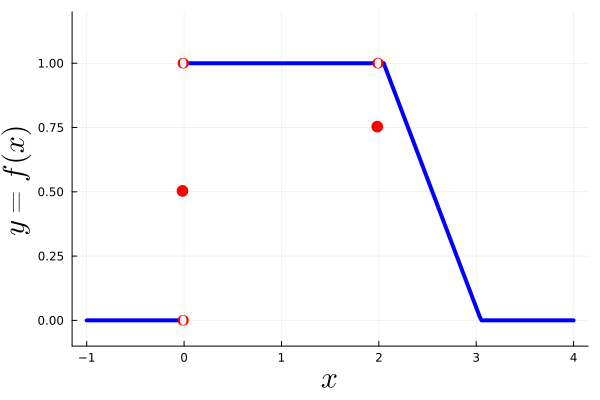
\includegraphics[width=0.6\columnwidth]{graphics/Chap04/LeftRightLimitExample01.png}%
    \caption[]{This oddly defined function will help us understand the notions of limit from the left and limit from the right at a point. The value of the function at $x=0$ is $0.5$, and its value at $x=2$ is $0.75$.}
    \label{fig:StrangeFunctionLeftRightLimits}
\end{figure}

\section{Intuition for Limits from the Left and the Right}
\label{sec:IntuitionLeftRightLimits}

To help with developing an intuitive feel for one-sided limits, consider the function
\begin{equation}
\label{eq:StrangeFunctionLeftRightLimits}
    f(x) :=  \begin{cases}
        0.0 & x < 0.0 \\
        0.5 & x = 0.0 \\
        1.0 & 0.0 < x < 2.0 \\
        0.75 & x = 2.0 \\
        1.0 - (x-2.0) & 2.0 < x \le 3.0 \\
        0.0 & x > 3.0
    \end{cases}
\end{equation}
as plotted in Fig.~\ref{fig:StrangeFunctionLeftRightLimits}. We have defined the value of the function at the origin to be neither zero nor one; in fact, $f(0)=0.5$. However, if we approach the origin from the left side, namely through negative values of $x$, the value of the function is constant and equal to zero. Hence, we say that the limit from the left at $x=0.0$ equals zero, and we denote this by
\begin{equation}
    \lim_{x \to 0^-} f(x) = 0.
\end{equation}
Here, the minus sign as a superscript on the right side of a value of $x$, currently $x_0=0$, indicates the limit is taken with values of $x$ that are strictly less than $x_0=0$, are never equal to $x_0$, but become ``arbitrarily close to $x_0$''.
Similarly, if we approach the origin from the right side, namely through small positive values of $x$, the value of the function is constant and equal to one. Hence, we say that the limit from the right at $x_0=0.0$ equals one, and we denote this by
\begin{equation}
    \lim_{x \to 0^+} f(x) = 1.
\end{equation}
Here, the plus sign as a superscript on the right side of a value of $x$, say $x_0$, indicates the limit is taken with values of $x$ that are strictly greater than $x_0=0$, are never equal to $x_0$, but become ``arbitrarily close to $x_0$''. Before we move on, let's note that the limit of the function from the left at the origin equals zero, its limit from the right equals one, and the value of the function at the origin is 0.5. The function is clearly discontinuous at the origin because there is a jump.

Let's next consider the behavior of the function near $x_0=2$.  If we approach $x_0=2$ from its left side, namely through values of $x$ strictly less than two, the value of the function is constant and equal to one. Hence, we say that the limit from the left at $x=2.0$ equals one, and we denote this by
\begin{equation}
    \lim_{x \to 2^-} f(x) = 1.
\end{equation}
Again, the minus sign as a superscript on the right side of a value of $x_0=2$ indicates the limit is taken with values of $x$ that are strictly less than $x_0=2$, are never equal to $x_0$, but become arbitrarily close to $x_0$.
Similarly, if we approach $x_0=2$ from the right side, namely through values of $x$ strictly greater than two, the value of the function is less than one but becomes arbitrarily close to one as $x$ approaches two. Hence, we say that the limit from the right at $x=2$ equals one, and we denote this by
\begin{equation}
    \lim_{x \to 2^+} f(x) = 1.
\end{equation}
Again, the plus sign as a superscript on the right side of $x_0=2$ indicates the limit is taken with values of $x$ that are strictly greater than $x_0$, are never equal to $x_0$, but become arbitrarily close to $x_0$. Before we move on, let's note that the limit of the function from the left at $x_0=2$ equals one, its limit from the right equals one, and the value of the function at $x_0=2$ is equal to 0.75. The function is discontinuous at $x_0=2$ because its value jumps from 1.0 to 0.75 at the point $x_0=2$. 

For our final case, let's consider the behavior of the function near $x_0=3$.  If we approach $x_0=3$ from its left side, namely through values of $x$ strictly less than three, the value of the function decreases to zero. Hence, we say that the limit from the left at $x=3$ equals zero, and we denote this by
\begin{equation}
    \lim_{x \to 3^-} f(x) = 0.
\end{equation}
As before, the minus sign as a superscript on the right side of a value of $x_0=3$ indicates the limit is taken with values of $x$ that are strictly less than $x_0=3$, are never equal to $x_0$, but become arbitrarily close to $x_0$. Similarly, if we approach $x_0=3$ from the right side, namely through values of $x$ strictly greater than three, the value of the function is constant and equal to zero. Hence, we say that the limit from the right at $x=3$ equals zero, and we denote this by
\begin{equation}
    \lim_{x \to 3^+} f(x) = 0.
\end{equation}
Again, the plus sign as a superscript on the right side of $x_0=3$ indicates the limit is taken with values of $x$ that are strictly greater than $x_0=3$, are never equal to $x_0$, but become arbitrarily close to $x_0$. Before we move on, let's note that the limit of the function from the left at $x_0=3$ equals zero, its limit from the right equals zero, and the value of the function at $x_0=3$ is equal to zero. The function is continuous at $x_0=3$ because its value does not undergo a jump as $x$ is varied near $x_0=3$. This is ``mathematically certified'' by the limit from the left, the limit from the right, and the function all having the same value at the point $x_0=3$. In fact, this property, namely, the two one-sided (left and right) limits existing and agreeing with the value of the function, holds for all $-1 < x \le 0$, $0 < x < 2$, and $2 < x < 4$; in other symbols, for all $x_0 \in \{ (-1, 4)~|~ x\neq 0 \text{ and } x\neq 2\}$, 
\[  \lim_{x \to x_0^-} f(x) = f(x_0) \text{ and } \lim_{x \to x_0^+} f(x) = f(x_0),\]
and this analysis agrees with our intuitive notion of the continuity of the function at those points. 


\bigskip

\begin{factColor}{Relation to Limits at $\pm \infty$}{relationSidedLimitsInfiniteLimits}
   We connect the one-sided limits to the work we did in Chapters~\ref{sec:LimitInfinityHard} and \ref{sec:LimitInfinityEasy}. The limit from the right is the same as the following (positive) infinite limit
    $$ \lim_{x \to x_0^+} f(x) = \lim_{\eta \to + \infty} f(x_0 + \frac{1}{\eta})$$
    and the limit from the left is the same as the corresponding negative infinite limit
    $$ \lim_{x \to x_0^-} f(x) = \lim_{\eta \to -\infty} f(x_0 + \frac{1}{\eta}).$$
    The key points are:
    \begin{itemize}
        \item $\frac{1}{\eta}$ is never exactly equal to zero, so we never evaluate the function at $x_0$;
        \item  as $\eta \to \infty$,  $x_0 + \frac{1}{\eta}$ approaches $x_0$ from the \textbf{right} because $x_0 + \frac{1}{\eta}> x_0$ for all $\eta >0$; and
        \item  as $\eta \to -\infty$,  $x_0 + \frac{1}{\eta}$ approaches $x_0$ from the \textbf{left} because $x_0 + \frac{1}{\eta}><x_0$ for all $\eta <0$.
    \end{itemize}
    
\textbf{Note:} If we make the substitution ${ h:=\frac{1}{\eta} }$, then ${ \eta \to +\infty \iff h \to 0^+ }$ (${h}$ decreases to zero through positive values, that is, ${h}$ approaches zero from the right) and ${ \eta \to -\infty \iff h \to 0^- }$ (because ${h}$ increases to zero through negative values, that is, ${h}$ approaches zero from the left).



\end{factColor}

\begin{figure}[htb]%
\centering
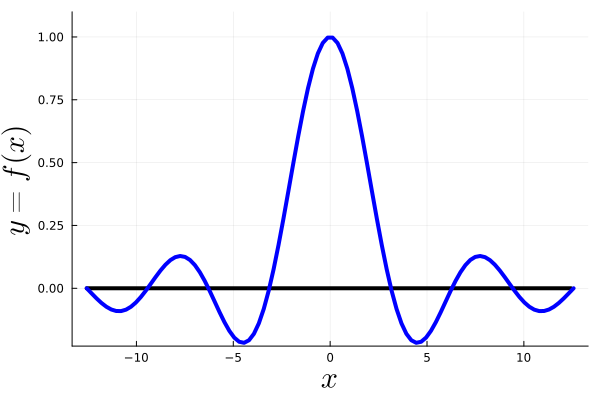
\includegraphics[width=0.6\columnwidth]{graphics/Chap04/sincFunction.png}%
    \caption[]{This is a plot of $\sin(x)/x$, a function that plays a starring role in Signal Processing. How is it possible to make sense of its value at the origin, where we have $0/0$? Inquiring minds want to know!}
    \label{fig:sincFunction}
\end{figure}
\bigskip

\begin{funColor}{How Might Limits Be Useful}{LimitsCanBeuseful}
   The function ${\rm sinc}(x):= \begin{cases}
       \frac{\sin(x)}{x} & x \ne 0 \\
       1 & x = 0
   \end{cases}$
   (pronounced ``sink'' or ``sync'') plays a big role in Signal Processing because it can be used to create\footnote{Michigan's EECS 216 Signals and Systems covers this material. In particular, it covers the Fourier Transform, which is the key to unlocking how a ${\rm sinc}$-function has anything to do with filtering noise from signals.} low-pass filters (i.e., filters that remove high-frequency ``noise'' from a data signal). Why is it defined to be one at the origin? \textbf{Limits give us a way to understand and analyze such conundrums as $\bm{0/0}$}. The function's graph is given in Fig.~\ref{fig:sincFunction}. \\
   
   This Chapter puts us on the road to understanding how to deal with ``$0/0$,'' while L'H\^opital's Rule in the next Chapter should clear up any remaining doubts.   
\end{funColor}



\section{Formal Definition of Limits from the Left and the Right}

We build off the observations presented in Fact~\ref{thm:relationSidedLimitsInfiniteLimits}.


% \begin{tcolorbox}[colback=mylightblue, title = {\bf One-sided Limits at Zero}, breakable]
% \begin{definition}
% \label{def:OneSidedlimitsAtZero}
% Suppose that $a < b$, $f:(a, b) \to  \real$ is a real-valued function, and both $L$ and $ R$ are (finite) real numbers. 

% \begin{enumerate}
% \renewcommand{\labelenumi}{(\alph{enumi})}
% \setlength{\itemsep}{.2cm}
%     \item For either $0\in I$ or $b=0$, the \textbf{limit of $f$ from the left at $0$} is equal to $L$ if, for all $\epsilon >0$ (no matter how small), there exists $\delta > 0$, such that for all $h\in I$ (belonging to the domain of the function), $-\delta < h < 0$ $\implies$ $|f(h) - L| \le \epsilon$. The left limit is denoted as
%     $$ \lim_{h \to 0^-} f(h) = L.$$ 

%       \item For either $0\in I$ or $a=0$, the  \textbf{limit from the right at $0$} is equal to $R$ if, for all $\epsilon >0$ (no matter how small), there exists $\delta > 0$, such that for all $h\in I$ (belonging to the domain of the function), $0 < h < \delta$ $\implies$ $|f(h) - R| \le \epsilon$. The right limit is denoted as
%     $$ \lim_{h \to 0^+} f(h) = R.$$ 
% \end{enumerate}

% \end{definition}
% \textbf{Notes:}
% \begin{itemize}

%     \item If the function is defined on something other than an interval of the form $(a, b)$, then it can always be restricted to an interval of the form $(a, b)$. We use this fact in the examples without commenting on it.

%    \item In the above, $h$ is a dummy variable. We can just as easily write $ \displaystyle \lim_{x \to 0^-} f(x) $, $ \displaystyle \lim_{y \to 0^+} f(y) $, etc.

%     \item As we take $\epsilon$ smaller and smaller, we typically need to take $\delta$ smaller and smaller. In other words, $\delta$ typically depends on $\epsilon$. It is sometimes useful to express this dependence as $\delta(\epsilon)$ or $\delta_\epsilon$, just as we did with $N(\epsilon)$ and $N_\epsilon$ when doing limits at infinity. 

%     \item In the definition, why did we need to insist that either $0 \in I$, $0=a$, or $0=b$? Well, suppose that $f:(1, 2) \to \real$ by $f(x) = \frac{x^2}{x^4 + 2x + 3} $. Then, the origin is far from the domain of definition of the function, and for all $0 < \delta < 1$, the set of $h$ that are smaller than $\delta$ and in the domain of the function is EMPTY! In other symbols, $\{ h\in I~|~ 0 < h < \delta \} = \emptyset$, and hence the conditions for the limit are vacuous\footnote{No points satisfy them, because you are playing with the empty set!}.

%     \item \textbf{Similar to limits as $x$ tends to infinity, most one-sided limits in Engineering can be computed by inspection; recall Chapter~\ref{sec:LimitInfinityEasy}. This will become more clear when we get to L'H\^{o}pital's Rule. For now, focus on the concept of how the function behaves as we approach the origin from the right or the left.}
% \end{itemize}
% \end{tcolorbox}

\begin{tcolorbox}[colback=mylightblue, title = {\bf One-sided Limits at Zero}, breakable]
\begin{definition}
\label{def:OneSidedlimitsAtZero}
Suppose that  $f:A \to  \real$ is a real-valued function, $A \subset \real$, and both $L$ and $ R$ are (finite) real numbers. 

\begin{enumerate}
\renewcommand{\labelenumi}{(\alph{enumi})}
\setlength{\itemsep}{.2cm}
    \item The \textbf{limit of $f$ from the left at $0$} is equal to $L$ if, for all $\epsilon >0$ (no matter how small), there exists $\delta > 0$, such that the open interval $(-\delta, 0) \subset A$ (i.e., is contained in the domain of definition of the function), and $-\delta < h < 0$ $\implies$ $|f(h) - L| \le \epsilon$. The left limit is denoted as
    $$ \lim_{h \to 0^-} f(h) = L.$$ 

      \item The \textbf{limit of $f$ from the right at $0$} is equal to $R$ if, for all $\epsilon >0$ (no matter how small), there exists $\delta > 0$, such that the open interval $(0, \delta) \subset A$ (i.e., is contained in the domain of definition of the function), and $0 < h < \delta$ $\implies$ $|f(h) - R| \le \epsilon$. The right limit is denoted as
    $$ \lim_{h \to 0^+} f(h) = R.$$ 
\end{enumerate}

\end{definition}
\textbf{Notes:}
\begin{itemize}

   \item In the above, $h$ is a dummy variable. We can just as easily write $ \displaystyle \lim_{x \to 0^-} f(x) $, $ \displaystyle \lim_{y \to 0^+} f(y) $, etc.

    \item As we take $\epsilon$ smaller and smaller, we typically need to take $\delta$ smaller and smaller. In other words, $\delta$ typically depends on $\epsilon$. It is sometimes useful to express this dependence as $\delta(\epsilon)$ or $\delta_\epsilon$, just as we did with $N(\epsilon)$ and $N_\epsilon$ when doing limits at infinity. 

    \item \textbf{Similar to limits as $x$ tends to infinity, most one-sided limits in Engineering can be computed by inspection, as in Chapter~\ref{sec:LimitInfinityEasy}, or with minor computations. This will become more clear when we get to L'H\^{o}pital's Rule. For now, focus on the concept of how the function behaves as we approach the origin from the right or the left. }
\end{itemize}
\end{tcolorbox}


\bigskip

\begin{example} 
\label{ex:LeftRightLimitsAtZero}
Compute the left and right limits at zero for the following functions.
\begin{enumerate}
\renewcommand{\labelenumi}{(\alph{enumi})}
\setlength{\itemsep}{.2cm}

  \item  $f(y) = y^2, y\in \real $

  \item $f(z) =  \begin{cases} 
       -1 + z^4 & z < 0\\
        0 & z = 0 \\
        1 + z^2 & z > 0
    \end{cases}$
    
    \item  $f(h) = \begin{cases} 
        \frac{h}{|h|}  & h \ne 0 \\
        \text{undefined} & h = 0
    \end{cases}$

    \item $f(x) = \begin{cases} 
        \sin(\frac{1}{x}) & x >0 \\
        0 & x \le 0
    \end{cases}$

    \end{enumerate}
    
\end{example}

\textbf{Solutions:} We first give solutions that use the epsilon-delta-definitions, and then provide a pointer for doing the limits by inspection. 

\begin{enumerate}
\renewcommand{\labelenumi}{(\alph{enumi})}
\setlength{\itemsep}{.2cm}

  \item  \Ans $\displaystyle \lim_{y \to 0^-} f(y) = 0$ and $\displaystyle \lim_{y \to 0^+} f(y) = 0$. \\

  Let $\epsilon>0$ be given and set $\delta := \sqrt{\epsilon}$. Then for all $-\delta < y < 0$, we have $|f(y)-L| = |y^2-0| = |y^2| = y^2 < (-\delta)^2 = \epsilon$, and hence the definition of the limit from the left is verified. \\

  Similarly, for all $0 < y < \delta$, we have $|f(y)-R| = |f(y)-0| = |y^2| = y^2 < (\delta)^2 = \epsilon$, and hence the definition of the limit from the right is verified. In this case, we could use the same $\delta$ for both sides of the limit.
 
  

  \item  \Ans $\displaystyle \lim_{z \to 0^-} f(z) = -1$ and $\displaystyle \lim_{z \to 0^+} f(z) = 1$. \\

  Let $\epsilon>0$ be given and set $\delta:= \sqrt[4]{\epsilon}$. Then for all $-\delta < z < 0$, we have $|f(z)-L| = |-1+z^4-(-1)| = |z^4| = z^4 < (-\delta)^4 = \epsilon$, and hence the definition of the limit from the left is verified. \\

  Let $\epsilon>0$ be given and set $\delta:= \sqrt{\epsilon}$ for all $0 < z < \delta$, we have $|f(z)-R| = |1+ z^2-1| = |z^2| = z^2 < (\delta)^2 = \epsilon$, and hence the definition of the limit from the right is verified.
  

    
    \item  \Ans $\displaystyle \lim_{h \to 0^-} f(h) = -1$ and $\displaystyle \lim_{h \to 0^+} f(z) = 1$. \\

  Let $\epsilon>0$ be given and set $\delta:= 27$. Then for all $-\delta < h < 0$, we have $|f(h)-L| = |\frac{h}{|h|}-(-1)| = |-1 - (-1)| = 0 < \epsilon$, and hence the definition of the limit from the left is verified. In this case, we can take $\delta$ to be any positive real number. It did not have to be small. You will understand why when you see the graph of $f(h)$ in Fig.~\ref{fig:LimitsLeftRIghtAtZero}-(c).\\

  Similarly, for all $0 < h < \delta$, we have $|f(h)-R| = |\frac{h}{|h|}-1| = |1 - 1| = 0 < \epsilon$, and hence the definition of the limit from the right is verified.


    \item \Ans $\displaystyle \lim_{x \to 0^-} f(x) = 0$ and $\displaystyle \lim_{x \to 0^+} f(x)$ does not exist.\\

    \textbf{Here is the insight:}  $ \displaystyle \lim_{x \to 0^+} \sin(\frac{1}{x}) =  \lim_{y \to + \infty} \sin(y)$, and we know that $\sin(y)$ oscillates forever between $-1$ and $+1$ as $y \to \infty$; hence, the limit from the right at zero does not exist.  Can we show this violates the existence of the limit, using epsilons and deltas? Of course! \\

    Let $R \in \real$, the candidate right limit, be arbitrary. Set $\epsilon = 0.25$ and let $\delta >0$ be arbitrary. We seek to show that there always exists $0 < x < \delta$ such that $|f(x)-R| > \epsilon$.\\
    
    Let $k$ be an even integer such that $0 < \frac{1}{k} < \delta$. Then $x_1:= \frac{1}{k \pi}$ and $x_2:= \frac{1}{(k + 0.5) \pi}$ satisfy $0 < x_2 <  x_1 < \delta$. These numbers were chosen because 
    $$ f(x_1) = \sin (k \pi) = 0 \text{ and } f(x_2) = \sin ( (k + 0.5) \pi) = \sin(\frac{\pi}{2}) = 1.$$ \\
    
    If $|f(x_1) -R| = |0 - R| = |R| > \epsilon$, then $R$ is not the right limit. Hence, suppose that $|R| \le \epsilon = 0.25$. Then, by the Reverse Triangle Inequality, $|f(x_2) - R| \ge \big|~ |f(x_2)| - |R| ~\big| \ge 1 - 0.25 = 0.75 > \epsilon$, and thus $R$ is not the right limit. Because $R$ was arbitrary, the right limit does not exist at zero. A zoom of the function's graph near the origin is shown below.
    \begin{center}
    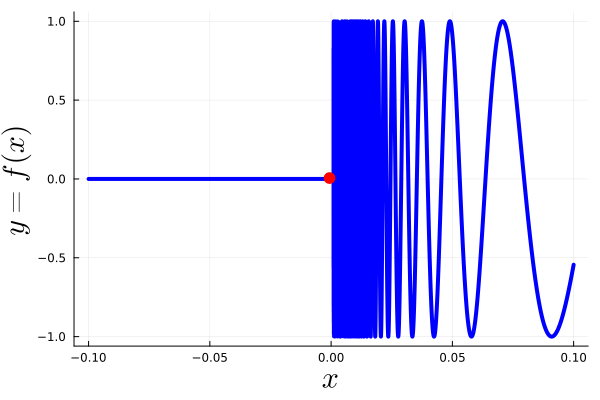
\includegraphics[width=0.45\columnwidth]{graphics/Chap04/LeftRightLimitAtZeroDZoom.png}
    \end{center}
    Because the limit from the left is ``obvious'', this completes the analytical solutions. \textbf{The solutions by inspection} proceed as in Chapter~\ref{sec:IntuitionLeftRightLimits}, using Fig.~\ref{fig:LimitsLeftRIghtAtZero}. You can trace the graph of each function to the left and right of zero to determine the limits.
    \end{enumerate}
    


\Qed

\begin{figure}[htb]%
\centering
\hfill
\subfloat[]{%
	\centering
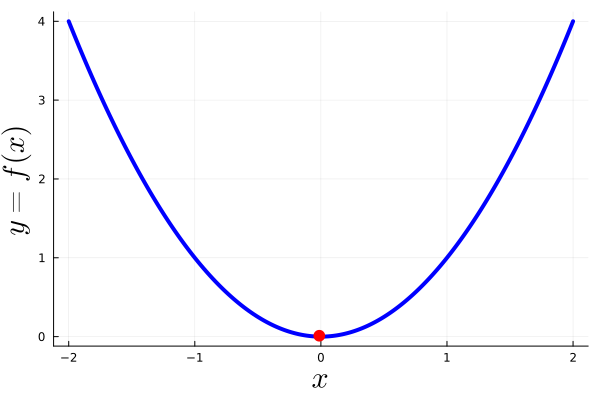
\includegraphics[width=0.45\columnwidth]{graphics/Chap04/LeftRightLimitAtZeroA.png}}%
\hspace{45pt}%
\subfloat[]{%
	\centering
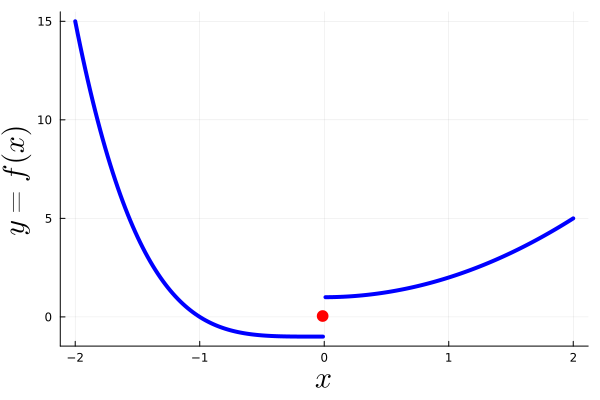
\includegraphics[width=0.45\columnwidth]{graphics/Chap04/LeftRightLimitAtZeroB.png}}%
\hfill
\subfloat[]{%
	\centering
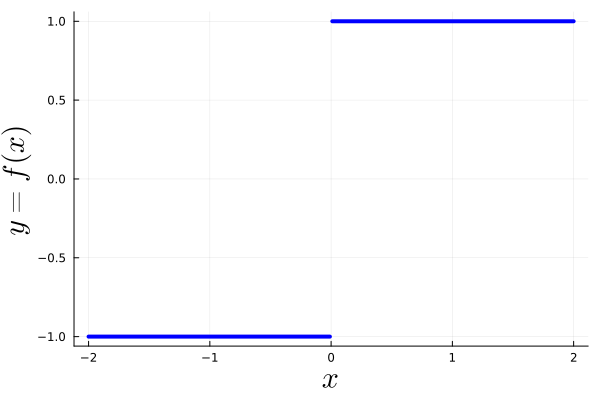
\includegraphics[width=0.45\columnwidth]{graphics/Chap04/LeftRightLimitAtZeroC.png}}%
\hfill
\subfloat[]{%
	\centering
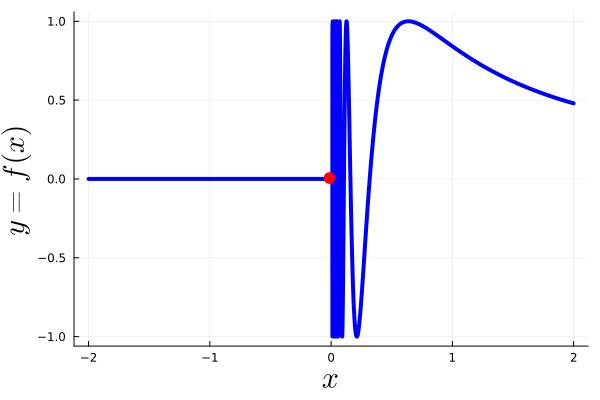
\includegraphics[width=0.45\columnwidth]{graphics/Chap04/LeftRightLimitAtZeroD.png}}%
    \caption[]{Graphs of the functions defined in Example~\ref{ex:LeftRightLimitsAtZero}, which treats left and right limits at zero. (a) The left and right limits are both equal to zero. (b) The left limit equals $-1$ and the right limit equals $+1$. (c) The left limit equals $-1$ and the right limit equals $+1$. (d) The left limit equals $0$ and the right limit is undefined because, from the right side of zero, the function oscillates between $-1$ and $+1$ an infinite number of times for $0 < x < \delta$, for any $\delta > 0$, no matter how small.}
    \label{fig:LimitsLeftRIghtAtZero}
\end{figure}

\begin{center}
\setlength{\fboxrule}{2pt}  % Setting the thickness of the border line
   \fbox{ \parbox{0.9\linewidth}{\textcolor{red}{\bf You can also estimate the limits numerically like this:} define $h[i] = \frac{1}{i}$ , $0 < i_{\rm min}\le i \le  i_{\rm max} $, for example, and then compute $f(h)$ and $f(-h)$ on the vector of values specified by $h$. This is illustrated in the next code block.
}} 
\end{center}


\begin{lstlisting}[language=Julia,style=mystyle]
eta = 100:1:1e4
h_Right = 1.0 ./eta
k = 2
y_Right = f.(h_Right,k)
p1 = plot(h_Right,y_Right, linewidth=4, color=:blue, label=false, guidefont=20)
plot!(xlabel=L"$x$", ylabel=L"$y=f(x)$")
h_Left = -h_Right
y_Left = f.(h_Left,k)
p1 = plot!(h_Left,y_Left, linewidth=4, color=:green, label=false, guidefont=20)
if k !=3
    annotate!(0, f(0,k), text(L"$\bullet$", :red, :center, 20))
end
ylims!(p1, (minimum(y_minus), maximum(y_Right)))

display(p1)

@show LeftLimit = y_Left[end]
@show RightLimit = y_Right[end]

png(p1, "LeftRightLimitAtZeroBSecondMethod")
\end{lstlisting}
\textbf{Output} 
\begin{verbatim}
LeftLimit = y_Left[end] = -0.9999999999999999
RightLimit = y_Right[end] = 1.00000001
\end{verbatim}

    \begin{center}
    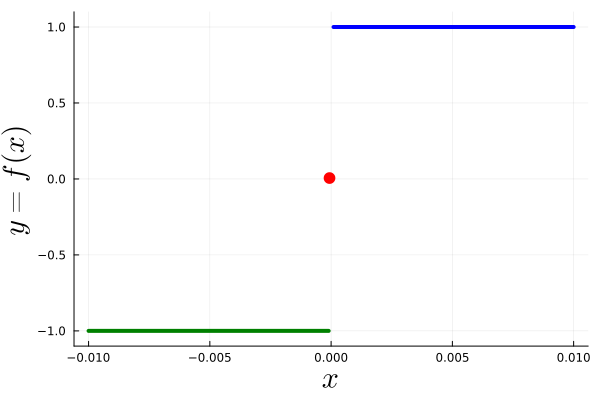
\includegraphics[width=0.6\columnwidth]{graphics/Chap04/LeftRightLimitAtZeroBSecondMethod.png}
    \end{center}

\bigskip

If the function diverges to infinity as we approach zero from the left or right, then finite limits will certainly not exist. We take care of this, just as we did for limits at infinity in Definition~\ref{def:LimitAtInfinity02}.


\begin{figure}[htb]%`
\centering
\subfloat[]{%
	\centering
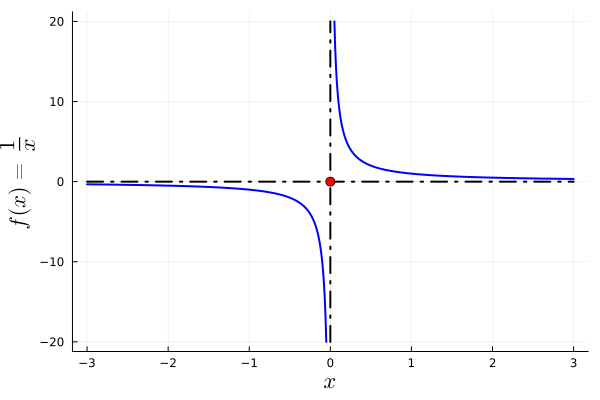
\includegraphics[width=0.45\columnwidth]{graphics/Chap04/UnboundedOneSidedLimits.png}}%
\subfloat[]{%
	\centering
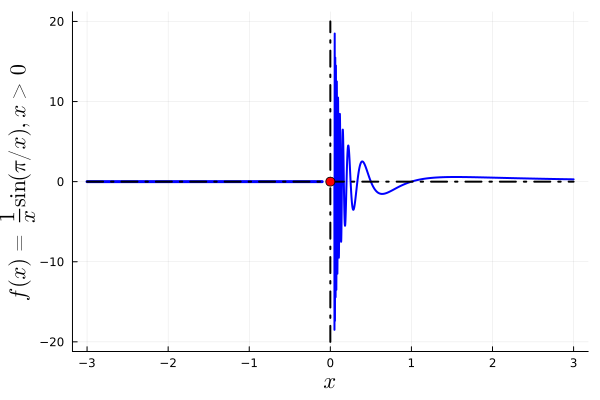
\includegraphics[width=0.45\columnwidth]{graphics/Chap04/UnboundedOneSidedLimitDoesNotExist.png}}%
\caption[]{Functions can also blow up as the origin is approached from the left or the right. (a) Both one-sided limits of $1/x$ exist but are $\pm \infty$. (b) The limit from the left exists and is bounded, while the limit from the right does not exist for $(1/x)\cdot \sin(\pi/x), x>0$.}
    \label{fig:OneSidedLimitsNotExisting}
\end{figure}

\bigskip


\begin{tcolorbox}[colback=mylightblue, title = {\bf Unbounded One-sided Limits at $0$}, breakable]

\begin{definition}
\label{def:UnboundedOneSidedlimitsAtZero}
Suppose that $A \subset \real$ and $f:A \to  \real$ is a real-valued function.

\begin{enumerate}
\renewcommand{\labelenumi}{(\alph{enumi})}
\setlength{\itemsep}{.2cm}
    \item The \textbf{limit of $f$ from the left at $0$} is equal to $\infty$ if, for all $0<N < \infty$ (no matter how large), there exists $\delta > 0$ such that the open interval $(-\delta, 0) \subset A$ (i.e., is contained in the domain of definition of the function, \textbf{and} $-\delta < h < 0$ $\implies$ $f(h)>N$. The left limit is then denoted as
    $$ \lim_{h \to 0^-} f(h) = \infty.$$ 
    Similarly, the \textbf{limit of $f$ from the left at $0$} is equal to $-\infty$ if, for all $0<N < \infty$  (no matter how large), there exists $\delta > 0$ such that he open interval $(0, \delta) \subset A$ (i.e., is contained in the domain of definition of the function), \textbf{and} $-\delta < h < 0$ $\implies$ $f(h)< -N$. The left limit is then denoted as
    $$ \lim_{h \to 0^-} f(h) = -\infty.$$ 

  \item The \textbf{limit of $f$ from the right at $0$} is equal to $\infty$ if, for all $0<N < \infty$ (no matter how large), there exists $\delta > 0$ such that the open interval $(0, \delta) \subset A$ (i.e., is contained in the domain of definition of the function, \textbf{and} $0 < h < \delta$ $\implies$ $f(h)>N$. The right limit is then denoted as
    $$ \lim_{h \to 0^+} f(h) = \infty.$$ 
    Similarly, the \textbf{limit of $f$ from the right at $0$} is equal to $-\infty$ if, for all $0<N < \infty$  (no matter how large), there exists $\delta > 0$ such that the open interval $(0, \delta) \subset A$ (i.e., is contained in the domain of definition of the function), \textbf{and} $0< h < \delta$ $\implies$ $f(h)< -N$. The right limit is then denoted as
    $$ \lim_{h \to 0^+} f(h) = -\infty.$$  
\end{enumerate}

\end{definition}

\end{tcolorbox}

\bigskip

\begin{example} For $f:\real \to \real$ by
$$f(x) = \begin{cases}
\frac{1}{x} & x\neq 0 \\
0 & x = 0,    
\end{cases}$$
compute the left and right limits at the origin.    
\end{example}

\textbf{Solution:} We provide first an analytical solution and then a numerical solution.\\

\Ans $ \displaystyle \lim_{h \to 0^-} f(h) = -\infty$. To prove this using the definition, let $0 < N < \infty$ be arbitrary. Then for $0<\delta < \frac{1}{N}$,
$$ -\delta < x < 0 \implies f(x) = \frac{1}{x} \le -\frac{1}{\delta} \le - \frac{1}{ \frac{1}{N}} = -N.$$
\\

\Ans $ \displaystyle \lim_{h \to 0^+} f(h) = \infty$. To prove this using the definition, let $0 < N < \infty$ be arbitrary. Then for $0<\delta < \frac{1}{N}$,
$$ 0<x<\delta \implies f(x) = \frac{1}{x} \ge \frac{1}{\delta} \ge \frac{1}{\frac{1}{N}} = N.$$
\\


\begin{lstlisting}[language=Julia,style=mystyle]
using Plots, LaTeXStrings

# Create a logarithmic scale of h values
k = 7 # 
h = 2.0 .^ range(-1, -k, step=-1)

f(x) = 1/x

# Limit from the right
p1 = scatter(h, f.(h), legend=false, markersize = 4, color=:red, guidefont=20)
plot!(xlabel = "h", ylabel = "f(h) = 1/h")
# Limit from the left
scatter!(-h, f.(-h), markersize = 4, color=:blue)
\end{lstlisting}
\textbf{Output} 

\begin{center}
    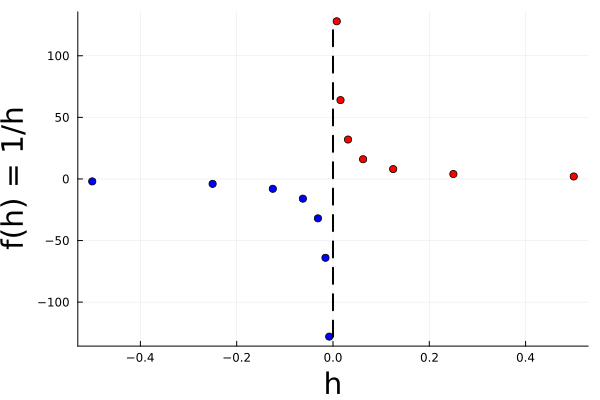
\includegraphics[width=0.45\columnwidth]{graphics/Chap04/SolutionLimitLeftRightAtZero.png}
\end{center}

\bigskip



% \begin{tcolorbox}[colback=mylightblue, title = {\bf One-sided Limits at a Point}, breakable]
% \begin{definition}
% \label{def:OneSidedlimits}
% Suppose that $a < b$, $f:(a, b) \to  \real$ is a real-valued function.
% \begin{enumerate}
% \renewcommand{\labelenumi}{(\alph{enumi})}
% \setlength{\itemsep}{.2cm}
%     \item For either $x_0\in (a, b)$ or $b=x_0$, the \textbf{limit from the left at $x_0$} is 
%     $$ \lim_{x \to x_0^-} f(x):=  \lim_{h \to 0^-} f(x_0+h). $$ 

%       \item For either $x_0\in (a, b)$ or $a=x_0$,  \textbf{limit from the right at $x_0$} is
%     $$ \lim_{x \to x_0^+} f(x) := \lim_{h \to 0^+} f(x_0+h). $$ 
% \end{enumerate}
% \end{definition}

% \textbf{Note:} The above is valid for finite limits and unbounded limits.

% \end{tcolorbox}

\begin{tcolorbox}[colback=mylightblue, title = {\bf One-sided Limits at a Point}, breakable]
\begin{definition}
\label{def:OneSidedlimits}
Suppose that  $f:A \to  \real$ is a real-valued function, $A \subset \real$, $x_0 \in \real$, and there exists $\delta >0$ such that the two open intervals $(x_0-\delta, x_0)$ and $(x_0, x_0 + \delta)$ are contained in $A$, the domain of definition of the function.
\begin{enumerate}
\renewcommand{\labelenumi}{(\alph{enumi})}
\setlength{\itemsep}{.2cm}
    \item The \textbf{limit from the left at $x_0$} is 
    $$ \lim_{x \to x_0^-} f(x):=  \lim_{h \to 0^-} f(x_0+h). $$ 

      \item The \textbf{limit from the right at $x_0$} is 
    $$ \lim_{x \to x_0^+} f(x) := \lim_{h \to 0^+} f(x_0+h). $$ 
\end{enumerate}

\end{definition}

\textbf{Notes:} 
\begin{itemize}
\item The above is valid for finite limits and unbounded limits.

\item  $(x_0-\delta, x_0) \subset A$ and $(x_0, x_0 + \delta) \subset A$ ensure that considering the limits from the left and right makes sense.

\end{itemize}

\end{tcolorbox}

\bigskip

\begin{example} Let's reuse the function that we studied in \eqref{eq:StrangeFunctionLeftRightLimits} and Fig.~\ref{fig:StrangeFunctionLeftRightLimits}, namely,
$$
    f(x) :=  \begin{cases}
        0.0 & x < 0.0 \\
        0.5 & x = 0.0 \\
        1.0 & 0.0 < x < 2.0 \\
        0.75 & x = 2.0 \\
        1.0 - (x-2.0) & 2.0 < x \le 3.0 \\
        0.0 & x > 3.0.
    \end{cases}
$$
Determine the limits from the left and right for 
\begin{enumerate}
\renewcommand{\labelenumi}{(\alph{enumi})}
\setlength{\itemsep}{.2cm}
    \item $x_0=0$

\item $x_0=2$, and

\item $x_0=3$.
\end{enumerate}    
\end{example}

\textbf{Solution:} We will take a numerical approach. We could plot the function near the specified values of $x_0$. We'll do something a bit more quantitative. We'll define a (finite) vector of $h$ values that terminates in very small values, e.g., on the order of $10^{-6}$. We'll also compute the \href{https://en.wikipedia.org/wiki/Mean}{mean} and (sample) \href{https://en.wikipedia.org/wiki/Standard_deviation}{standard deviation} of the function evaluated $x_0 \pm h$, namely
\begin{itemize}
    \item $h[i]=\frac{1}{i+i_{\rm min}}$, $1 \le i \le N$, $i_{\rm min}>0$ a constant.
    \item $y_R[i]:=f(x_0 + h[i])$
    \item $\mu_R := \frac{1}{N} \cdot \sum_{i=1}^N  y_R[i]$ (mean value)
    \item $\sigma_R :=  \sqrt{\frac{1}{N-1} \cdot \sum_{i=1}^N  \left( y_R[i]  - \mu_R \right)^2}$ (sample standard deviation)
\end{itemize}
and similarly for the left-sided limit. If the function has a right limit at $x_0$, then $y_R$ should be nearly a constant for $N$ large. Hence, when
\begin{itemize}
    \item $\mu_R \approx y_R[N]$ and
    \item  $\sigma_R \approx 0$,
\end{itemize}
the numerical evidence \textbf{suggests} that $y_R[N]$ is a good estimate of the limit.

\bigskip

\begin{lstlisting}[language=Julia,style=mystyle]
function f(x)
    if x < 0
        y = -1.0
    elseif abs(x)<1e-12
        y = 0.0
    elseif (0 < x < 2)
        y = 1.0
    elseif abs(x-2.0)<1e-12
        y = 0.75
    elseif (2 < x <= 3.0)
        y = 1.0 - (x - 2.0)
    else 
        y = 0.0
    end
    return y
end
#
using Statistics
eta = 1e3:1e3:1e6
h_Right = (1.0)./ eta
h_Left = -h_Right
x0Vec = [0.0 2.0 3.0]

delta = h_Right[end]

@show delta
println(" ")

for k = 1:length(x0Vec)
    x0 = x0Vec[k]
    y_Left = f.(x0 .+ h_Left)
    y_Right = f.(x0 .+ h_Right)
    #
    @show x0
    @show limitLeft = y_Left[end]
    @show meanLeft = mean(y_Left)
    @show stdDevLeft = std(y_Left)
    println("--------")
    @show limitRight = y_Right[end]
    @show meanRight = mean(y_Right)
    @show stdDevRight = std(y_Right)    
    println(" ")
    println(" ")
    #
end
\end{lstlisting}
\textbf{Output} 
\begin{verbatim}
delta = 1.0e-6
 
x0 = 0.0
limitLeft = y_Left[end] = -1.0
meanLeft = mean(y_Left) = -1.0
stdDevLeft = std(y_Left) = 0.0
--------
limitRight = y_Right[end] = 1.0
meanRight = mean(y_Right) = 1.0
stdDevRight = std(y_Right) = 0.0
 
 
x0 = 2.0
limitLeft = y_Left[end] = 1.0
meanLeft = mean(y_Left) = 1.0
stdDevLeft = std(y_Left) = 0.0
--------
limitRight = y_Right[end] = 0.9999989999999999
meanRight = mean(y_Right) = 0.9999925145291394
stdDevRight = std(y_Right) = 3.9868430925503734e-5
 
 
x0 = 3.0
limitLeft = y_Left[end] = 1.000000000139778e-6
meanLeft = mean(y_Left) = 7.4854708605545105e-6
stdDevLeft = std(y_Left) = 3.986843092550373e-5
--------
limitRight = y_Right[end] = 0.0
meanRight = mean(y_Right) = 0.0
stdDevRight = std(y_Right) = 0.0
\end{verbatim}

We see that the estimated numerical limits correspond well to what we computed previously in Chapter~\ref{sec:IntuitionLeftRightLimits}, when all we knew to do was read values from a graph. In each case, $y[N] \approx \mu$ and $\sigma \approx 0$.
\Qed

Let's now try the more challenging example of $\sin(\frac{1}{x}), x>0$ and zero otherwise. 

\begin{example} 
Determine the limits from the left and right for $g(x):= \sin(\frac{1}{x}), x> 0$ and $g(x)=0, x\le 0$, for $x_0 \in \{ 0.0,  \frac{1}{\pi},  \frac{2}{\pi}\}$.
\end{example}
\textbf{Solution:}
\begin{lstlisting}[language=Julia,style=mystyle]
eta = 1e3:1e3:1e6
h_Right = (1.0)./ eta
h_Left = -h_Right
x0Vec = [0.0 1.0/pi 2.0/pi]

g(x) = x > 0 ? sin(1/x) : 0.0

delta = h_Right[end]

@show delta
println(" ")

for k = 1:length(x0Vec)
    x0 = x0Vec[k]
    y_Left = g.(x0 .+ h_Left)
    y_Right = g.(x0 .+ h_Right)
    #
    @show x0
    @show limitLeft = y_Left[end]
    @show meanLeft = mean(y_Left)
    @show stdDevLeft = std(y_Left)
    println("--------")
    @show limitRight = y_Right[end]
    @show meanRight = mean(y_Right)
    @show stdDevRight = std(y_Right)    
    println(" ")
    println(" ")
    
    println(" ")
    #
end
\end{lstlisting}
\textbf{Output} 
\begin{verbatim}
delta = 1.0e-6
 
x0 = 0.0
limitLeft = y_Left[end] = 0.0
meanLeft = mean(y_Left) = 0.0
stdDevLeft = std(y_Left) = 0.0
--------
limitRight = y_Right[end] = -0.34999350217129294
meanRight = mean(y_Right) = -0.00011524369884409064
stdDevRight = std(y_Right) = 0.7075827861802105
 
 
 
x0 = 0.3183098861837907
limitLeft = y_Left[end] = -9.869635406884313e-6
meanLeft = mean(y_Left) = -7.392953161190493e-5
stdDevLeft = std(y_Left) = 0.0003944103587102789
--------
limitRight = y_Right[end] = 9.86957339451198e-6
meanRight = mean(y_Right) = 7.382758963882898e-5
stdDevRight = std(y_Right) = 0.0003925579978142143
 
 
 
x0 = 0.6366197723675814
limitLeft = y_Left[end] = 0.999999999996956
meanLeft = mean(y_Left) = 0.9999999949842888
stdDevLeft = std(y_Left) = 1.0037167987310087e-7
--------
limitRight = y_Right[end] = 0.999999999996956
meanRight = mean(y_Right) = 0.9999999950072798
stdDevRight = std(y_Right) = 9.976893600410653e-8
\end{verbatim}

As we suspected from Example~\ref{ex:LeftRightLimitsAtZero}-(d), the left limit at the $x_0=0$ exists and is equal to zero, but the right limit does not exist. This shows up in the numerical calculations by
\begin{itemize}
    \item $|\mu_R - y_R[N]| \approx 0.35 $ is ``large''; and
    \item  $\sigma_R \approx 0.708$ is also large.
\end{itemize}
These observations are compatible with the extreme oscillations on the right side of the origin, as seen in Fig.~\ref{fig:LimitsLeftRIghtAtZero}-(d). All other one-sided limits exist.
\Qed

\bigskip

We next illustrate unbounded one-sided limits at a point.

\bigskip

\begin{example} 
\label{ex:LimitsTangentOfx}
Determine the limits from the left and right at $x_0 \in \{ 0.0,  -\frac{\pi}{2},  -\pi\}$ for $g(x):= \tan(x), (x \mod \pi ) \neq  \frac{\pi}{2}$ (i.e., $x$ is not an odd multiple of $\pi/2$) and $g(x)=0$ otherwise. 
\end{example}

    \begin{center}
    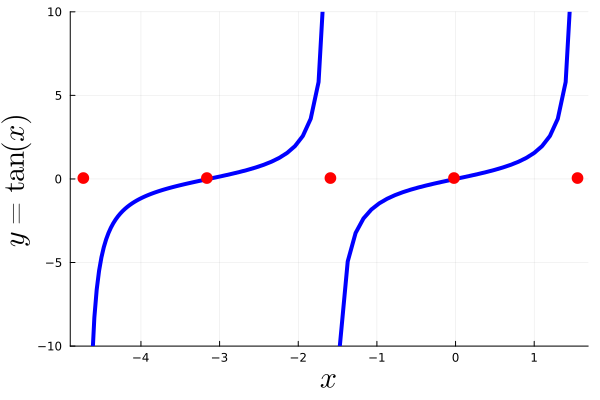
\includegraphics[width=0.45\columnwidth]{graphics/Chap04/LeftRightLimitTangent.png}
    \end{center}
    
\textbf{Solution:}
Because $(x \mod \pi ) = \frac{\pi}{2} \implies \sin(x)= \pm 1$ and $\cos(x) = 0$, we expect unbounded limits at these points (numerator is non-zero and the denominator is equal to zero). Similarly, because $(x \mod \pi ) = 0 \implies \sin(x)= 0$ and $\cos(x) = \pm 1$, we expect the limits to be zero. Indeed, based on the plot, we can see the one-sided limits at $x_0=0$ and $x_0 = -\pi$ all exist and are equal to zero, which is confirmed by the numerical calculations below. Moreover, the limit from the left at $-\frac{\pi}{2}$ appears to be $+\infty$, while the limit from the right appears to be $-\infty$, consistent with the ``analytical'' study of the problem. 

\begin{lstlisting}[language=Julia,style=mystyle]
using Statistics
eta = 1e3:1e3:1e6
h_Right = (1.0)./ eta
h_Left = -h_Right
x0Vec = [0.0 -pi/2 -pi]

g(x) = abs(x % pi) >1e-10  ? tan(x) : 0.0

delta = h_Right[end]

@show delta
println(" ")

for k = 1:length(x0Vec)
    x0 = x0Vec[k]
    y_Left = g.(x0 .+ h_Left)
    y_Right = g.(x0 .+ h_Right)
    #
    @show x0
    @show limitLeft = y_Left[end]
    @show meanLeft = mean(y_Left)
    @show stdDevLeft = std(y_Left)
    println("--------")
    @show limitRight = y_Right[end]
    @show meanRight = mean(y_Right)
    @show stdDevRight = std(y_Right)    
    println(" ")
    println(" ")
    
    println(" ")
    #
end
\end{lstlisting}
\textbf{Output} 
\begin{verbatim}
delta = 1.0e-6
 
x0 = 0.0
limitLeft = y_Left[end] = -1.0000000000003333e-6
meanLeft = mean(y_Left) = -7.485471261235949e-6
stdDevLeft = std(y_Left) = 3.986843990838751e-5
--------
limitRight = y_Right[end] = 1.0000000000003333e-6
meanRight = mean(y_Right) = 7.485471261235949e-6
stdDevRight = std(y_Right) = 3.986843990838751e-5
 
 
 
x0 = -1.5707963267948966
limitLeft = y_Left[end] = 1.0000000001431657e6
meanLeft = mean(y_Left) = 500500.000018453
stdDevLeft = std(y_Left) = 288819.43611785874
--------
limitRight = y_Right[end] = -1.000000000020701e6
meanRight = mean(y_Right) = -500499.9999775702
stdDevRight = std(y_Right) = 288819.4360824532
 
 
 
x0 = -3.141592653589793
limitLeft = y_Left[end] = -1.0000000000176466e-6
meanLeft = mean(y_Left) = -7.485471261117652e-6
stdDevLeft = std(y_Left) = 3.986843990838485e-5
--------
limitRight = y_Right[end] = 1.000000000262576e-6
meanRight = mean(y_Right) = 7.485471261362585e-6
stdDevRight = std(y_Right) = 3.986843990838485e-5
\end{verbatim}
\Qed

\bigskip

\begin{tcolorbox}[title = {This can be the Point where the Wheels Come off the Track!}, sharp corners, colback=lightgold, colframe=black, coltitle=white, breakable, fonttitle=\bfseries]

Wheels off the track! Why? Because this Chapter is difficult. It speaks to the heart of Calculus. Once you master limits and continuity of functions, everything else in the book seems easier by comparison. It's maybe a good time to assess where you stand. Are your study habits really good enough? You have been in school for, like, forever. But have you really learned how to learn? While you should seek out resources on your own, here are a few suggestions:
\begin{itemize}
\item \href{https://youtu.be/rhgwIhB58PA}{The Biggest Myth In Education} by Veritasium. Speaks about learning ``styles''.
\item \href{https://youtu.be/n3kIPsO0Qv8}{Math is Hard for Everyone} and \href{https://www.youtube.com/watch?v=d5gJ1xvTQv4}{Don't Be A Math Imposter} by the Math Sorcerer. \textbf{Scan the comments before watching the videos.}
\item Basic things are important:
\begin{itemize}
   \item Go to Office Hours the moment you catch yourself falling behind or being confused by any topic. Avoiding office hours and spending 2-3 weeks to figure it out yourself will only hurt you. It's okay to ask for help or an extra explanation!
\item Read the relevant textbook material before attending (watching) the lecture (you can see what topics will be covered on the course schedule in the syllabus).
\item Review the homework solutions once they are posted to learn from your mistakes.
\item Don't wait until the last minute on a project. Complete small chunks of it over the span of 2 weeks.
\end{itemize}
\item \textcolor{blue}{\bf Put in the time: (4 hours lectures and recitation)~ + ~(8 hours assignments and studying) = 12 hours per week for a typical student in the course.} \textcolor{red}{\bf Are you typical? Lying to yourself is the worst.}
\item Your author struggled Y1 in College (lied to himself in semester one) and had to right the ship in semester two or lose essential scholarships and quit college. Here is what worked for him (one person out of the seven or eight billion on the planet).  
\begin{itemize}
    \item Carefully review all extracurricular activities. Trim to only the ones you need to stay sane. Once your results match your expectations, you can slowly add more fun back in. This is called feedback control! 
    \item Scan the Chapter before attending (or watching) the lecture so that you know what to expect and where the challenging points are; should take 15 minutes or less.
    \item Take essential notes during the lecture, keeping in mind that the instructor's notes are posted after each lecture.
    \item Before the next lecture, rewrite and condense your notes to one side of a single page. The book has the full details on most material. You do not need all of that in your notes. Being thoughtful about condensing your notes provides a third pass on the material. Along with the first two passes, scanning the Chapter before the lecture and attending or watching the lecture, you should be good to go. If not, you know what questions to ask during Office Hours!
\end{itemize}
\end{itemize}

\end{tcolorbox}

\bigskip



\section{The Power of Continuity Done Right} 

Now that we've done the hard work of understanding limits, we have the tools to move beyond our folksy definition of ``a function is continuous if we can draw its graph without lifting our pencil from the paper''. \textcolor{blue}{\bf The real definition of continuity at a point will provide a major benefit to us when it comes to evaluating limits and computing integrals}.

\subsection{Continuity at a Point and Continuous Everywhere on the Domain of Definition}

\begin{tcolorbox}[colback=mylightblue, title = {\bf Continuity at a Point and Continuous Everywhere}, breakable]
\begin{definition}
\label{def:Continuity}
Suppose that $I \subset \real$ is an open interval, that is, $I$ is either $(a, b), (a, \infty), (-\infty, b)$, or $(-\infty, \infty)$ as in 
 Definition~\ref{def:SymbolsAndSets}.
\begin{enumerate}
\renewcommand{\labelenumi}{(\alph{enumi})}
\setlength{\itemsep}{.2cm}
    \item A function $f:I \to \real$ is \textbf{continuous at $x_0 \in I$} if the two one-sided limits at $x_0$ exist and agree with the value of the function at $x_0$. In other symbols, 
\begin{equation}
\label{eq:continuousAtx0}
    \begin{aligned}
        \lim_{x \to x_0^-} f(x) &= f(x_0), \text{ and} \\
        \lim_{x \to x_0^+} f(x) & = f(x_0).
    \end{aligned}
\end{equation}

\bigskip

\emstat{For intervals containing an endpoint, such as $[a, b]$, $[a, b)$, $[a, \infty)$, $(a, b]$, and $[b, \infty)$, we have to treat the endpoints differently, but all other points in the interval are treated as above.}

    \item For $I$ a closed or half-open interval as highlighted above and $x_0 \in I$ \textbf{not an endpoint}, $f$ is continuous at $x_0$ if the conditions in \eqref{eq:continuousAtx0} hold. At the endpoints of the interval, only one of the one-sided limits makes sense. Hence, $f$ is \textbf{continuous at $x_0=a$, a lower endpoint,} if 
    $$\displaystyle \lim_{x \to a^+} f(x) = f(a),$$ and $f$ is \textbf{continuous at $x_0=b$, an upper endpoint,} if 
    $$\displaystyle \lim_{x \to b^-} f(x) = f(b).$$

    \item A function $f$ that is not continuous at $x_0$ is said to be \textbf{discontinuous at $x_0$} or $x_0$ is said to be \textbf{a point of discontinuity} of the function. 
   

      \item If $f$ is continuous at each point $x_0\in I$, its domain of definition, then \textbf{$f$ is simply said to be continuous}. If you want to say that $f$ is \textbf{continuous everywhere in (or on) its domain of definition}, that is fine too!

      \item If $f$ is not continuous at all points of its domain of definition, then it is \textbf{discontinuous}. It only takes one point of discontinuity to make a function discontinuous. 
\end{enumerate}
\end{definition}

\begin{rem} For $x_0\in \real$, it can NEVER be the case that $f(x_0)=\pm \infty$ because \textbf{the codomains of our functions contain only real numbers}. We recall that $\infty$ is a concept and not a number. Limits can equal $\infty$ because we allow functions to grow without bound, such as the function $f:\real \to \real$ by $f(x)=x$ or $f:(0, \infty) \to (0, \infty)$ by $f(x) = \frac{1}{x}$. \\
  
\end{rem}

\end{tcolorbox}

\bigskip

\emstat{Equation~\ref{eq:continuousAtx0} can be rearranged as
\begin{equation}
\label{eq:continuousAtx0Equivalent}
\begin{aligned}
        \lim_{x \to x_0^-} \left(f(x)- f(x_0) \right) &=0, \text{ and} \\
        \lim_{x \to x_0^+} \left( f(x) -f(x_0) \right) &=0.
    \end{aligned} 
\end{equation}
We'll use this equivalence in Example~\ref{ex:ContinuityViaLeftRightLimits}.}
 

\bigskip

\begin{example}
\label{ex:ContinuityViaLeftRightLimits}
For the following functions, determine, if any exist, their points of discontinuity. If there are no points of discontinuity, then state the function is continuous everywhere in its domain of definition.

    \begin{enumerate}
\renewcommand{\labelenumi}{(\alph{enumi})}
\setlength{\itemsep}{.2cm}
    \item $f:\real \to \real$ by $f(x) = x^3$.

     \item $f:[2, \infty) \to \real$ by $f(x) = x^2$.

     \item  $f:\real \to \real$ by $f(x) =
     \begin{cases} x^3 & x \ge 0 \\
                   x^2 & x < 0.
    \end{cases} $

         \item  $f:\real \to \real$ by $f(x) =
     \begin{cases} 1 + x & x \ge 0 \\
                   x^2 & x < 0.
    \end{cases} $

      \item  $f:[0, \infty) \to \real$ by $f(x) = \begin{cases}
        \sin(\frac{1}{x}) & x >0 \\
        0 & x = 0
    \end{cases}$

     \item $f:(0, \infty) \to \real$ by $f(x) = \log_a(x)$, where $a>1$.

    \end{enumerate}
\end{example}

\textbf{Solutions:}

\begin{enumerate}
\renewcommand{\labelenumi}{(\alph{enumi})}
\setlength{\itemsep}{.2cm}
    \item \Ans $x^3$ is continuous at all points of its domain of definition. We show this via the definition. Let $x_0 \in \real$ be arbitrary. Then, 
    \begin{align*}
       \lim_{x \to x_0^-} x^3&:=  \lim_{h \to 0^-} (x_0+h)^3  =  \lim_{h \to 0^-} \left( x_0^3 + 3 h x_0^2 + 3 h^2 x_0 + h_0^3\right) = x_0^3 + 0 + 0 + 0=  x_0^3\\
        \lim_{x \to x_0^+} x^3 &:=  \lim_{h \to 0^+} (x_0+h)^3  =  \lim_{h \to 0^+} \left( x_0^3 + 3 h x_0^2 + 3 h^2 x_0 + h_0^3\right) = x_0^3 + 0 + 0 + 0=  x_0^3.
    \end{align*}
    Because $x_0$ was arbitrary, $x^3$ is continuous at all points of its domain of definition.  \textcolor{blue}{\bf Note that here, we did the limits by inspection after some simple algebra (namely, the Binomial Theorem)}.

    \item \Ans $(\bullet)^2:[2, \infty) \to \real$ is continuous at all points of its domain of definition. We show this via the definition. We first consider $2 < x_0 < \infty$, but otherwise arbitrary. Then, 
    \begin{align*}
       \lim_{x \to x_0^-} x^2:=  \lim_{h \to 0^-} (x_0+h)^2  =  \lim_{h \to 0^-} \left( x_0^2 + 2 h x_0 + h_0^2\right) = x_0^2 + 0 + 0 =  x_0^2\\
        \lim_{x \to x_0^+} x^2:=  \lim_{h \to 0^+} (x_0+h)^2  =  \lim_{h \to 0^+} \left( x_0^2 + 2 h x_0 + h_0^2\right) = x_0^2 + 0 + 0 =  x_0^2.
    \end{align*}
    So far, so good! Let's now let $x_0=2$. We only check the limit from the right, namely,
    $$ \lim_{x \to 2^+} x^2:=  \lim_{h \to 0^+} (2+h)^2  =  \lim_{h \to 0^+} \left( 4 + 4 h  + h_0^2\right) = 4 + 0 + 0 =  4 = x_0^2. $$
    Because we checked continuity at all points of its domain, $(\bullet)^2:[2, \infty) \to \real$ is continuous at all points of its domain of definition. \textcolor{blue}{\bf Once again, the limits themselves were computed by inspection.} 

    \item \Ans $f(x) = 
     \begin{cases} x^3 & x \ge 0 \\
                   x^2 & x < 0.
    \end{cases} $
    is continuous at all points of its domain of definition. We solve this one a bit differently, because continuity for $x>0$ and $x<0$ can be checked the same as we did for parts (a) and (b). The only point that seems a bit different is the origin, but because $x^3$ and $x^2$ both vanish at the origin, there should not be a problem; to be sure, we'll check it anyway!  
    \begin{align*}
       \lim_{x \to 0^-} x^2&:=  \lim_{h \to 0^-} (0+h)^2  =  \lim_{h \to 0^-} h^2 = 0 =  0^2\\
        \lim_{x \to 0^+} x^3 &:=  \lim_{h \to 0^+} (0+h)^2  =  \lim_{h \to 0^+} h^3 = 0 =  0^3.
    \end{align*}
    Hence, the definition of continuity at a point is met for all points of the domain of definition of the function.

     \item \Ans $f(x) = 
     \begin{cases} 1 + x & x \ge 0 \\
                   x^2 & x < 0.
    \end{cases} $ is discontinuous at $x_0=0$ and continuous everywhere else. Once again, checking the limits for all $x_0\neq 0$ is straightforward, and we leave that to the learner. For $x_0=0$, we see that
     \begin{align*}
       \lim_{x \to 0^-} x^2 &:=  \lim_{h \to 0^-} (0+h)^2  =  \lim_{h \to 0^-} h^2 = 0 \neq f(0)=1\\
        \lim_{x \to 0^+} 1+x &:=  \lim_{h \to 0^+} (1+0+h)  =  \lim_{h \to 0^+} 1+h = 1 =  f(0).
    \end{align*}
    Because the left limit at zero is not equal to the value of the function at zero, the function is discontinuous at the origin. {\bf It was not necessary to compute the limit from the right; we simply did it for extra practice.}

    \item \Ans $f(x) = \begin{cases} 
        \sin(\frac{1}{x}) & x >0 \\
        0 & x = 0
    \end{cases}$ is discontinuous at the origin, and continuous everywhere else in its domain of definition, meaning, it is continuous for all $x>0$. The function is discontinuous at $x_0=0$ because we showed earlier, in Example~\ref{ex:LeftRightLimitsAtZero}, that $ \displaystyle \lim_{x \to 0^+} \sin(1/x)$ does not exist. Hence, the limit from the right cannot equal the value of the function, which is zero. \\

    For $x>0$, set $y:= \frac{1}{x}$. Then $y>0 \iff x>0$ reduces us to whether $\sin(y)$ is continuous or not for $y>0$. But we ``know'' from experience that it is continuous, so we're done! Really? For now, in any case. A formal proof can be given using trig identities and the bounds given in Fig.~\ref{fig:TrigFunctionsAndArea}.

    \item \Ans $f(x) = \log_a(x)$, where $a>1$ is continuous everywhere in its domain of definition, which we know is $(0, \infty)$. We first show continuity at the origin and then use the pattern established for the special case to handle the general case. Recall from Prop.~\ref{thm:PropertiesLogs}, for all $a >1$, $\log_a(1) = 0$. Hence, we need to show that both
    \begin{align*}
        \lim_{h \to 0^-} \log_a(1+h) &= 0, \text{ and} \\
         \lim_{h \to 0^+} \log_a(1+h) &= 0.
    \end{align*}
    This limit is less obvious than the previous limits; hence, we give an epsilon-delta proof: Let $\epsilon>0$ be arbitrary. We seek $\delta > 0$ such that
     \begin{align*}
        -\delta < h < 0 &\implies |\log_a(1+h)| \le  \epsilon, \text{ and} \\
        0< \delta < h &\implies  |\log_a(1+h)| \le  \epsilon = 0,
    \end{align*}
    where we note that we can use different values for $\delta$ in the two cases. From Prop.~\ref{thm:triangleAndReverseTriangleInequality}-(c), we have that 
     $$  |\log_a(1+h)| < \epsilon \iff -\epsilon < \log_a(1+h) < \epsilon.$$
     Because, for $a>1$, $a^x$ is strictly monotonically increasing on $(-\infty, \infty)$, taking the exponential preserves the inequalities; hence, 
      $$   -\epsilon < \log_a(1+h) < \epsilon \iff a^{-\epsilon} < 1+h < a^{\epsilon}.$$ 
      Therefore\footnote{For all $a>1$, $a^x < 1 \iff x<0 $.}, 
     $$  |\log_a(1+h)| < \epsilon \iff \underbrace{a^{-\epsilon} -1}_{< 0} < h < \underbrace{a^{\epsilon}-1}_{>0},$$
     which implies that
          \begin{align*}
        -\delta < h < 0 &\implies |\log_a(1+h)| \le  \epsilon, \text{ when } \delta = 1 - a^{-\epsilon}, \text{ and} \\
        0< \delta < h &\implies  |\log_a(1+h)| \le  \epsilon,  \text{ when } \delta = a^{\epsilon}-1,
    \end{align*}
    establishing continuity at the origin. To show continuity at a general $x>0$, we want to show that the left and right limits as $h$ tends to zero of $\log_a(x+h) - \log_a(x) =0$. But, using log properties, 
    $$\log_a(x+h) - \log_a(x) = \log_a \left( \frac{x+h}{x} \right) =  \log_a \left( 1 + \frac{h}{x} \right).$$ 
    Because $x>0$, if we define $\bar{h}:=\frac{h}{x}$, then $\bar{h} \to 0^- \iff h \to 0^-$ and $\bar{h} \to 0^+ \iff h \to 0^+$. Hence, 
        \begin{align*}
        \lim_{h \to 0^-} \log_a(1+\frac{h}{x}) &=  \lim_{\bar{h} \to 0^-} \log_a(1+\bar{h}), \text{ and} \\
         \lim_{h \to 0^+} \log_a(1+\frac{h}{x}) &=  \lim_{\bar{h} \to 0^+} \log_a(1+\bar{h}),
    \end{align*}
    reducing the problem to the case we have already considered, namely, continuity at $x_0 = 1$.

\end{enumerate}
    \Qed

\subsection{Two-sided Limits and Continuous Functions}  

You might imagine that if the limit from the left and the right both exist at a point, then you can combine them into a single limit. And you can! 

\begin{tcolorbox}[colback=mylightblue, title = {\bf Two-sided Limit at a Point}, breakable]
 To set the stage, consider a function $f:A \to \real$ where $A$ is a subset of $\real$, $x_0 \in \real$, and there exists $\delta>0$ such that both $(x_0 - \delta, x_0 ) \subset A$ and $(x_0 , x_0 + \delta) \subset A$. Then $x_0 + h \in A$ for all  $0<|h|<\delta$, meaning we can evaluate 
\begin{align*}
    \lim_{h \to 0^-} &f(x_0 + h ), \text{ and}, \\
    \lim_{h \to 0^+} &f(x_0 + h ),
\end{align*}
the left and right limits. 

\begin{definition} \label{def:TwoSidedLimitAtZero} Suppose that $f:A \to \real$, where $A$ is a subset of $\real$ and $x_0 \in A$. Then the limit as $x$ approaches $x_0$ exists and is equal to $L$, a finite real number, if for all $\epsilon>0$, there exists $\delta >0$, such that $0 < |h| < \delta \implies |f(x_0+h) -L| \le \epsilon.$ The limit is denoted as
$$ \lim_{x \to x_0} f(x) = L.$$
\end{definition}

\textbf{``Two-sided limits'' are typically called ``limits,'' with the adjective ``two-sided'' dropped.} It's only in the case of a one-sided limit that you need to call it out its \href{https://en.wikipedia.org/wiki/Sinistral_and_dextral}{chirality} (``sidedness'' or handedness of the limit).
\end{tcolorbox}

\bigskip



\begin{factColor}{Equivalence between a Two-sided Limit and Two One-sided Limits}{equivalenceBetween2SidedLimitAndTwo1SidedLimits}

Two of one, versus one of the other: the following are equivalent statements for $|L| < \infty$:
    \begin{enumerate}
\renewcommand{\labelenumi}{(\alph{enumi})}
\setlength{\itemsep}{.2cm}

    \item $\displaystyle \lim_{x \to x_0^-} f(x) = L$ and $\displaystyle  \lim_{x \to x_0^+} f(x) = L$. 

    \item $\displaystyle  \lim_{x \to x_0} f(x) = L. $
    \end{enumerate}

 \textbf{Notes:} 
Statements being equivalent means $(a) \iff (b)$, where we note that \textbf{(a) is true} if, and only if, \textbf{both one-sided limits exist and are equal to $\bm{L}$}. Just as with a one-sided limit, we never evaluate the function at $x_0$ when evaluating a two-sided limit. \textcolor{blue}{\bf In theory, you can replace every ``limit'' with two one-sided limits. However, this is not common practice and some faculty or GSIs may mark you wrong for using two one-sided limits in place of a single (two-sided) limit!} People fear what they do not fully understand. You are expected to fall into line...ha! 
\end{factColor}

\bigskip

Using the above Fact, continuity of a function at a point can be checked with a single (two-sided) limit instead of two one-sided limits. We'll leave that to you. What we'll do instead is give the classical epsilon-delta definition of a function being continuous at a point and then \textbf{relate all of the (commonly seen) definitions of continuity at a point}. 

\bigskip

\begin{tcolorbox}[colback=mylightblue, title = {\bf Classical Definition of Continuity at a Point}, breakable]

\begin{definition} \label{def:ClassicalDefinitionContinuityAtPoint} Suppose that $f:I \to \real$, where $I$ is an interval and $x_0 \in A$. Then  $f$ is continuous at $x_0$ if for all $\epsilon>0$, there exists $\delta >0$, such that 
$$\{ x ~~|~~ |x-x_0| < \delta\} \subset I  ~~\textcolor{red}{\bf and }~~ |x-x_0| < \delta \implies |f(x) -f(x_0)| \le \epsilon.$$

\textbf{Note:} If $ \{ x \in \real~~|~~ |x-x_0| < \delta\} \not \subset I$, then it does not make sense to evaluate the function at all of these points because some of them (at least) are not in the domain of the function! 
\end{definition}

\end{tcolorbox}

\bigskip

\begin{factColor}{Equivalent Ways to Define Continuity  at a Point}{equivalentContinuityCharacterizations}

The following statements are equivalent for a function $f:I \to \real$, where $I$ is an interval:
    \begin{enumerate}
\renewcommand{\labelenumi}{(\alph{enumi})}
\setlength{\itemsep}{.2cm}
    \item $f$ is continuous at $x_0$ by Def.~\ref{def:ClassicalDefinitionContinuityAtPoint}.

    \item $\displaystyle \lim_{x \to x_0^-} f(x) = f(x_0)$ and $\displaystyle \lim_{x \to x_0^+} f(x) = f(x_0)$, meaning that Def.~\ref{def:Continuity} of continuity at a point holds. 

    \item  $\displaystyle \lim_{x \to x_0} f(x) = f(x_0)$ (equivalent to the above because two one-sided limits are always equivalent to a single one-sided limit.)
    \end{enumerate}    
\end{factColor}

More examples of using limits and checking continuity with the modified formulations would be repetitive. Instead, let's list some common continuous functions.


\begin{propColor}{Common Continuous Functions}{CommonContFuns}

The following functions are continuous for all $x\in \real$ \textcolor{blue}{unless indicated otherwise}:\\

\textbf{Polynomial Functions}
\begin{itemize}
  \item Constant function: $ f(x) = c $
  \item Linear function: $ f(x) = ax + b $
  \item Quadratic function: $ f(x) = ax^2 + bx + c $
  \item Higher-degree polynomials: $ f(x) = a_nx^n + a_{n-1}x^{n-1} + \cdots + a_1x + a_0 $
\end{itemize}

\textbf{Trigonometric Functions}
\begin{itemize}
  \item Sine: $ f(x) = \sin(x) $
  \item Cosine: $ f(x) = \cos(x) $
  \item Tangent \textcolor{blue}{(continuous except at odd multiples of $ \pm \frac{\pi}{2} $)}: $ f(x) = \tan(x) $
\end{itemize}

\textbf{Power Function}
\begin{itemize}
  \item Power \textcolor{blue}{(continuous for $x > 0$ and $y \in \real)$}: $ f(x) = x^y $
\end{itemize}

\textbf{Exponential and Logarithmic Functions}
\begin{itemize}
  \item Exponential: $ f(x) = a^x $ (where $ a > 1 $)
  \item Natural Exponential: $ f(x) = e^x $
  \item Logarithm \textcolor{blue}{(continuous for $ x > 0 $)}: $ f(x) = \log_a(x) $ (where $ a > 1 $)
  \item Natural Logarithm \textcolor{blue}{(continuous for $ x > 0 $)}: $ f(x) = \ln(x) $
\end{itemize}

\textbf{Rational Functions (subject to domain restrictions)}
\begin{itemize}
  \item $ f(x) = \frac{p(x)}{q(x)} $ where $ p(x) $ and $ q(x) $ are polynomials and \textcolor{blue}{$ q(x) \neq 0 $ (means, rational functions are continuous for all $x\in \real$ such that $q(x)\neq 0$)}
\end{itemize}

\textbf{Root Functions}
\begin{itemize}
  \item Square Root \textcolor{blue}{(continuous for $ x \geq 0 $)}: $ f(x) = \sqrt{x} $
  \item Cube Root: $ f(x) = \sqrt[3]{x} $
  \item $ n $-th Root \textcolor{blue}{(continuous for $ x \geq 0 $ if $ n \in \nat$ is even, all $ x \in \real$ if $ n \in \nat$ is odd)}: $ f(x) = \sqrt[n]{x} $
\end{itemize}


\textbf{Other Special Functions}
\begin{itemize}
  \item Absolute Value: $ f(x) = |x| $
  \item Triangle: $f(x) = \tri(x)$
  \item Radial Basis Function: $ f(x) = e^{-\frac{(x-x_c)^2}{s^2}} $
  \item Gaussian (Normal Distribution) with mean $\mu$ and standard deviation $\sigma$:
$f(x) = \frac{1}{\sqrt{2 \pi \sigma^2}} e^{-\frac{(x-\mu)^2}{2 \sigma^2}} $

\end{itemize}

\end{propColor}

\bigskip

\begin{tcolorbox}[title = {Reassurance on Limits and Continuity}, sharp corners, colback=lightgold, colframe=black, coltitle=white, breakable, fonttitle=\bfseries]
As a practicing engineer with a BSE, you will rarely, if ever, need to use the epsilon-delta definition of a limit or continuity at a point. You will mostly handle these concepts by ``inspection'', and if you're a good engineer, you'll ``mostly get the answers right''. \\

Depending on your goals, if you go to graduate school, being comfortable with theory may become more important. Hence, we've tried so far in the textbook to represent the perspective of both kinds of learners: those who chose engineering out of a love for math and physics per se and those who like math and physics, but really came to engineering out of a desire to build stuff and improve the lives of people. Your author has advised amazing graduate students on both ends of the spectrum and everywhere in between. Everyone's path is different. That is why Michigan's Robotics Graduate Program starts with \href{https://grizzle.robotics.umich.edu/education/rob501.html}{ROB 501 Mathematics for Robotics}: to level the mathematical playing field for all learners. \\

If, out of personal interest, you are paying close attention to the theoretical discussions so far (e.g., the proofs at the end of each Chapter), then you may wish to target Michigan's MATH 451 course (or its equivalent). Where we pull back and hesitate on the details, MATH 451 goes full speed ahead. If you want the extra rigor now: \href{https://youtu.be/AfrnYS5S8VE}{Rigorous limit proof ultimate study guide: ($\epsilon$-$\delta$, $\epsilon$-$N$, $M$-$\delta$, and $M$-$N$ proofs)} by \bprp.
\end{tcolorbox}




% \begin{example}
%     \label{ex:ListOfContinuousDiscontinuousFunctions}
%     State which of the following common functions are continuous everywhere on their domain and which are discontinuous. For functions labeled as discontinuous, give at least one point of discontinuity.
%         \begin{enumerate}
% \renewcommand{\labelenumi}{(\alph{enumi})}
% \setlength{\itemsep}{.2cm}

% \item $f:\real \to \real$ by $f(x) = x^k$, where $k$ is an odd positive integer.

% \item $f:\real \to [0, \infty)$ by $f(x) = x^k$, where $k$ is an even positive integer.

% \item $f:[0, \infty)] \to \real$ by $f(x) = \sqrt[n]{x}$, for $n\ge 1$ an integer.

% \item $f:\real \to [0, 1]$ by $f(x) = \sin(x)$.

% \item $f:\real \to [0, 1]$ by $f(x) = \cos(x)$.

% \item $f:(0, \infty) \to (0, \infty)$ by $f(x) = x^y$, for $y \in \real$, $y \neq 0$.

% \item $f:\real \to (0, \infty)$ by $f(x) = e^x$.

% \item $f:(0, \infty) \to \real$ by $f(x) = \ln(x)$.

% \item $f:(0, \infty) \to \real$ by $f(x) = \log_a(x)$, $a>1$.

% \item $f:(-\frac{\pi}{2} , \frac{\pi}{2}) \to \real$ by $f(x) = \tan(x)$.

% % \item $f:\real \to [0, 1]$ by $f(x) = \UnitStep(x)$.

% \item $f:\real \to [0, 1]$ by $f(x) = u_{\rm s}(x)$.

% \item $f:\real \to [0, 1]$ by $f(x) = \rect(x)$.

% \item $f:\real \to [0, 1]$ by $f(x) = \tri(x)$.

% \item 

% \end{enumerate}    
% \end{example}

\subsection{Key Properties of Continuous Functions or Why We Care about Continuity}

For the purpose of developing and understanding the fundamentals of Calculus, the following Proposition ranks among the most important results in this course. 

\bigskip

\begin{propColor}{Taking Limits Inside a Function}{LimitInsideFunction}
    Consider two functions $g:X \to Y$ and $f:Y \to Z$, where $X$, $Y$, and $Z$ are subsets of $\real$. Suppose that $f$ is continuous at a point $y_0 \in Y$. Then, the following hold:
\begin{enumerate}
\renewcommand{\labelenumi}{(\alph{enumi})}
\setlength{\itemsep}{.2cm}

\item If $x_0 \in \real$ and $\displaystyle \lim_{x \to x_0} g(x) = y_0$ (i.e., the limit exists and equals $y_0$), then $\displaystyle \lim_{x \to x_0} f(g(x)) = f(\lim_{x \to x_0} g(x)) = f(y_0). $ \textbf{We say the limit can be taken ``inside'' the function $f$.}

\item Similarly, if $\displaystyle \lim_{x \to \infty} g(x) = y_0$, then $\displaystyle \lim_{x \to \infty} f(g(x)) = f(\lim_{x \to \infty} g(x)) = f(y_0). $  

\item If $\displaystyle \lim_{x \to -\infty} g(x) = y_0$, then $\displaystyle \lim_{x \to -\infty} f(g(x)) = f(\lim_{x \to -\infty} g(x)) = f(y_0). $ 
\end{enumerate}
In short, if $g(x)$ has a limit (as $x$ approaches a finite point or as $x$ approaches $\pm \infty$), and $f$ is continuous at the limit of $g$ (i.e., $y_0$), then, when evaluating a limit of $f(g(x)) = f\circ g(x)$,  the limit can be taken inside the function $f$ and applied directly to $g$.  
\end{propColor}

\bigskip
You may enjoy the video \href{https://youtu.be/H2RQC4PxEM0}{Mu Prime Math} ``When can we switch the limit and function?''
\bigskip

\begin{example}
\label{ex:LimitsUsingcontinuity}
Use Prop.~\ref{thm:LimitInsideFunction} to evaluate the following limits. In each case, as part of your solution, identify the functions $g:X \to Y$ and $f:Y \to Z$, as well as the limit point of $g$, which we have been calling $y_0$.
\begin{enumerate}
\renewcommand{\labelenumi}{(\alph{enumi})}
\setlength{\itemsep}{.2cm}

\item $ \displaystyle \lim_{x \to 0} \sin\left( \frac{x}{1 + x^2} \right)$

\item $ \displaystyle \lim_{x \to \frac{\pi}{2} } \frac{3 + \sin^3(x)}{\sin^2(x) + 3 \sin(x) + 4}$

\item $ \displaystyle \lim_{x \to \infty} \ln(e^{-2x} + e^{-x} + 1) $
\end{enumerate}    
\end{example}

\textbf{Solutions:}

\begin{enumerate}
\renewcommand{\labelenumi}{(\alph{enumi})}
\setlength{\itemsep}{.2cm}

\item \Ans $ \displaystyle \lim_{x \to 0} \sin\left( \frac{1 + x}{1 + x^2} \right) = \sin(1) \approx 0.8415$. \\

We define $f:\real \to \real$ by $f(y) = \sin(y)$,  $g: \real \to \real$ by $g(x) = \frac{1 + x}{1 + x^2}$, and note that  $\displaystyle \lim_{x \to 0} g(x) = \lim_{x \to 0} \frac{1 + x}{1 + x^2} = 1=:y_0$. The limit exists because $g$ is continuous everywhere on its domain of definition per Prop.~\ref{thm:CommonContFuns} Common Continuous Functions. Finally, also by Prop.~\ref{thm:CommonContFuns}, $f(y)$ is continuous everywhere and hence at the point $y_0:=1$.

\item \Ans $ \displaystyle \lim_{x \to \frac{\pi}{2} } \frac{3 + \sin^3(x)}{\sin^2(x) + 3 \sin(x) + 4} = \frac{1}{2}$ (because $\sin(\pi/2) = 1$). \\

We define $f:\real \to \real$ by $f(y) = \frac{3 + y^3}{y^2 + 3 y + 4} $,  $g: \real \to \real$ by $g(x) = \sin(x)$, and note that  $\displaystyle \lim_{x \to \frac{\pi}{2} } g(x) = \lim_{x \to \frac{\pi}{2} } \sin(x)= 1.0 =:y_0$. The limit exists because $g$ is continuous everywhere on its domain of definition per Prop.~\ref{thm:CommonContFuns} Common Continuous Functions. Finally, also by Prop.~\ref{thm:CommonContFuns}, $f(y)$ is continuous everywhere and hence at the point $y_0:=0$.

\item \Ans $ \displaystyle \lim_{x \to \infty} \ln(e^{-2x} + e^{-x} + 1) = 0$.\\

This problem requires, given what we know at this point in the Chapter, two applications of Prop.~\ref{thm:LimitInsideFunction}. We will write $ \ln(e^{-2x} + e^{-x} + 1)$ as the composition of three functions, $ \ln(e^{-2x} + e^{-x} + 1) = : f(g(h(x)))$, where
\begin{align*}
    f:(0, \infty) \to \real ~\text{ by } ~f(z) = \ln(z) \\
    g:(0, \infty) \to (1, \infty) ~\text{ by } ~g(y) = y^2 + y + 1\\
    h:\real \to (0, \infty) ~\text{ by } ~h(x) = e^{-x},
\end{align*}
where we note that $g(h(x)) = (e^{-x})^2 + e^{-x} + 1 = e^{-2x} + e^{-x} + 1$ because $\left(  a^\alpha \right)^{\beta} = a^{\alpha \cdot \beta}$ for all $a>0$, and real numbers $\alpha $ and $\beta$.\\

All three functions are continuous everywhere on their domains of definition. Moreover, 
\begin{align*}
\lim_{x \to \infty} h(x) & =  \lim_{x \to \infty} e^{-x} = 0 =: y_0 \\
 g(y_0) = g(0) & = 1=: z_0 \\
 f(z_0) = f(1) & = \ln(1) = 0.
\end{align*}

Therefore, 
\begin{align*}
    \lim_{x \to \infty} \ln(e^{-2x} + e^{-x} + 1) & = \lim_{x \to \infty} f(g(h(x)))\\
    & = f ( \lim_{x \to \infty}~ g(h(x)) )\\
     & = f (g ( ~\underbrace{\lim_{x \to \infty}~ h(x)}_{y_0 = 0} ~) )\\
    & =  f ( ~\underbrace{g \left( 0 \right)}_{z_0 = 1} ~) \\
    & = f(1) \\
    & = \ln(1) \\
    & = 0.
\end{align*}
\end{enumerate}

\textbf{Note:} All of these limits can be approximated numerically using the same techniques we have already demonstrated.

\Qed

\bigskip
\emstat{The above problem was mainly an exercise in writing a ``complicated'' function as a composition of simpler functions. The next two problems are more representative of how Prop.~\ref{thm:LimitInsideFunction} is typically used. Their solutions will illustrate how a change of variable can make an apparently intractable problem become tractable.}

\bigskip


\begin{example} 
\label{ex:eToPowerxDerivativeNatLogx}

Using the fact that $\displaystyle \lim_{n \to \infty} \left( 1 + \frac{1}{n} \right)^n =: e$, compute the following limits:
\begin{enumerate}
\renewcommand{\labelenumi}{(\alph{enumi})}
\setlength{\itemsep}{.2cm}

\item $\displaystyle \lim_{n \to \infty} \left( 1 - \frac{1}{n} \right)^{-n}$;

\item $\displaystyle \lim_{n \to \infty} \left( 1 + \frac{x}{n} \right)^n$, where $x \in \real$ is arbitrary; and

\item $\displaystyle \lim_{h \to 0} \frac{\ln(x + h) - \ln(x)}{h} $, where $x >0$.

\end{enumerate}    

\end{example}


\emstat{\textbf{Hints:} For (a), note that $\left( 1 - \frac{1}{n} \right)^{-1} = \left( \frac{n-1}{n} \right)^{-1} =  \left( \frac{n}{n-1} \right) = \left( \frac{n-1+1}{n-1} \right) = 1 + \frac{1}{n-1}$. Also, Prop.~\ref{thm:LimitProdRatio} is helpful. Finally, remember your power rules! \\

For (b), when $x=0$, the limit is clearly one, leaving two cases to investigate, $x>0$ and $x < 0$. First, assume $x > 0$ and use the substitution $m:=\frac{n}{x}$ and look for the power function $f: (0, \infty) \to (0, \infty)$ by $f(y) = y^x$. Note that here, the variable is $y$, and $x$ is a fixed positive constant. Follow a similar pattern for $x < 0$.\\

For (c), recall your logarithm rules for $\ln(x) \pm \ln(y)$ and $\ln(x^y)$. Try the substitution, $n := \frac{1}{h}$.}

\textbf{Solutions:} 

\begin{enumerate}
\renewcommand{\labelenumi}{(\alph{enumi})}
\setlength{\itemsep}{.2cm}

\item \Ans $\displaystyle \lim_{n \to \infty} \left( 1 - \frac{1}{n} \right)^{-n} = e$.\\

Using the Hint, we have
\begin{align*}
    \lim_{n \to \infty} \left( 1 - \frac{1}{n} \right)^{-n} & = \lim_{n \to \infty} \left( \left( 1 - \frac{1}{n} \right)^{-1} \right)^n \\
    & = \lim_{n \to \infty} \left( 1 + \frac{1}{n-1} \right)^{n}.
\end{align*}
This is very close to the limit for $e$, but we're not quite there yet. We do a change of variable $m := n-1$ so that
$$n \to \infty \iff m \to \infty. $$
Hence, 
\begin{align*}
    \lim_{n \to \infty} \left( 1 - \frac{1}{n} \right)^{-n} & =\lim_{n \to \infty} \left( 1 + \frac{1}{n-1} \right)^{n} \\
    & = \lim_{m \to \infty} \left( 1 + \frac{1}{m} \right)^{m+1} \\
    & = \lim_{m \to \infty}~ \underbrace{\left( 1 + \frac{1}{m} \right)^{m}}_{f(m)} ~\cdot ~\underbrace{\left( 1 + \frac{1}{m} \right)}_{g(m)},    
\end{align*}
settings us up to apply Prop.~\ref{thm:LimitProdRatio}, because
$$ \lim_{m \to \infty} g(m) = 1 \text{ and }  \lim_{m \to \infty} f(m) = e.$$
We conclude therefore that $\displaystyle \lim_{n \to \infty} \left( 1 - \frac{1}{n} \right)^{-n} = e$.\\

\textbf{Note:} Can you show that for all integers $k\ge 1$, $\displaystyle \lim_{n \to \infty} \left( 1 + \frac{1}{n \pm k} \right)^{n} = \lim_{n \to \infty} \left( 1 + \frac{1}{n} \right)^{n \pm k}= e$? The key point is that $k$ is a fixed (finite) value when applying  Prop.~\ref{thm:LimitProdRatio}.

\item \Ans $\displaystyle \lim_{n \to \infty} \left( 1 + \frac{x}{n} \right)^n = e^x$.\\

Using the hint, we assume $x>0$ and set $m:=\frac{n}{x}$ so that 
$$ n = m \cdot x ~~\text{ and } m \to \infty \iff n \to \infty.$$
Making the substitution, we have
\begin{align*}
    \lim_{n \to \infty} \left( 1 + \frac{x}{n} \right)^n & = \lim_{m \to \infty} \left( 1 + \frac{1}{m} \right)^{m \cdot x} \\
    & =  \lim_{m \to \infty}  \left( \left( 1 + \frac{1}{m} \right)^{m} \right) ^x.
\end{align*}
We define $f(y):= y^x$ and note that it is continuous for all $y > 0$. Hence, 
\begin{align*}
    \lim_{n \to \infty} \left( 1 + \frac{x}{n} \right)^n & = \lim_{m \to \infty}  \left( \left( 1 + \frac{1}{m} \right)^{m} \right) ^x \\
    & =   \left( \lim_{m \to \infty}  \left( 1 + \frac{1}{m} \right)^{m} \right) ^x ~~\text{(take limit inside}~f) \\
    & = (e)^x ~~\text{(recognizing the limit)}\\
    & = e^x.
\end{align*}

We still have $x < 0$ to go, but the pattern is now pretty clear. Note that because $x < 0$, $x = -|x|$ and $|x| \neq 0$. Hence, we set $m:=\frac{n}{|x|}$ so that 
$$ n = m \cdot |x| ~~\text{ and } m \to \infty \iff n \to \infty.$$
Making the indicated substitution, we have
\begin{align*}
    \lim_{n \to \infty} \left( 1 + \frac{x}{n} \right)^n & = \lim_{n \to \infty} \left( 1 - \frac{|x|}{n} \right)^n \\
    & = \lim_{m \to \infty} \left( 1 - \frac{1}{m} \right)^{m \cdot |x|} \\
    & =  \lim_{m \to \infty}  \left( \left( 1 - \frac{1}{m} \right)^{-m} \right) ^{-|x|},
\end{align*}
where on the last line, we used our power rules. We define $f(y):= y^x = y^{-|x|}$ and note that it is a continuous function of $y$ for all $y > 0$. Hence, 
\begin{align*}
    \lim_{n \to \infty} \left( 1 + \frac{x}{n} \right)^n & = \lim_{m \to \infty}  \left( \left( 1 - \frac{1}{m} \right)^{-m} \right) ^ {-|x|} \\
    & =   \left( \lim_{m \to \infty}  \left( 1 - \frac{1}{m} \right)^{-m} \right) ^{-|x|} ~~\text{(take limit inside}~f) \\
    & = (e)^{-|x|} ~~\text{(recognizing the limit)}\\
    & = e^{-|x|} \\
    & = e^x ~~(\text{because~~x = -|x|)}.
\end{align*}

\item \Ans For all $x>0$, $\displaystyle \lim_{h \to 0} \frac{\ln(x + h) - \ln(x)}{h} = \frac{1}{x}$.\\

Using our logarithm rules, 
\begin{align*}
     \frac{\ln(x + h) - \ln(x)}{h} &= \frac{1}{h} \ln \left( \frac{x+h}{x} \right) \\
     & = \ln \left( \left(\frac{x+h}{x} \right)^\frac{1}{h} \right) \\
     & =  \ln \left( \left( 1 + \frac{h}{x} \right)^\frac{1}{h} \right).
\end{align*}
We make the substitution $n := \frac{1}{h}$ so that
$$  n \to \infty \iff h \to 0^+.$$
Using this substitution, we have 
\begin{align*}
    \lim_{h \to 0^+} \frac{\ln(x + h) - \ln(x)}{h} & = \lim_{h \to 0^+}  \ln \left( \left( 1 + \frac{h}{x} \right)^\frac{1}{h} \right) \\
    &= \lim_{n \to \infty} \ln \left( \left( 1 + \frac{1}{n x} \right)^n \right)\\
    & = \ln  \left( \lim_{n \to \infty}  \left( 1 + \frac{1}{n x} \right)^n  \right) ~~(\text{taking the limit inside because } \ln(x) \text{ is continuous}) \\
    &  = \ln \left(  e^\frac{1}{x} \right) ~~(\text{recognizing the limit by part (b) of this problem})\\
    & = \frac{1}{x} ~~\text{(using logarithm rules)}.
\end{align*}

In theory, we should now consider $\displaystyle \lim_{h \to 0^-} \frac{\ln(x + h) - \ln(x)}{h}$, but we leave it to the learner.

\end{enumerate} 

\Qed

\bigskip
This following (challenging) limit is the key to understanding the definite integral, $\int_a^b e^x dx$.
\bigskip

\begin{example} 
\label{ex:KeyExponentialLimit} 
Evaluate $\displaystyle \lim_{h \to 0} \frac{e^h - 1}{h}$.     
\end{example}

\textbf{Solution:} \Ans $\displaystyle \lim_{h \to 0} \frac{e^h - 1}{h} = 1$.\\

\emstat{At first blush, none of the methods we have covered so far seems applicable. This is more typical of how real engineering problems go. Initially, you are totally convinced that nothing you learned in School is useful for the problem at hand, but then, all of a sudden, you see how the problem can be tackled if you look at it the right way. Here, we need to make a change of variable and apply logarithm rules, even though there is no logarithm in sight! }

The power move is to define $u:= e^h - 1$ so that $e^h = u + 1 \iff h = \ln(1 + u)$. We note $\ln(x)$ is continuous everywhere on $(0, \infty)$, and that $h \to 0 \iff u \to 0$. With this substitution, we have 
$$\displaystyle \lim_{h \to 0} \frac{e^h - 1}{h} = \lim_{u \to 0} \frac{u}{\ln(1+u)} = \lim_{u \to 0} \frac{1}{ \frac{1}{u} \cdot \ln(1+u)}. $$
From our logarithm properties, recall that
$$y \cdot \ln(x) = \ln(x^y),$$
and hence, $ \frac{1}{u} \cdot \ln(1+u)  = \ln\left((1+u)^{\frac{1}{u}} \right)$, yielding
$$\displaystyle \lim_{h \to 0} \frac{e^h - 1}{h} =  \lim_{u \to 0} \frac{1}{\ln\left((1+u)^{\frac{1}{u}} \right)}.$$
Now we have to stare at the problem a bit and realize that $(1+u)^{\frac{1}{u}}$ looks vaguely familiar to us. In fact, if we defined $n := \frac{1}{u}$, we'd have 
$$ (1+u)^{\frac{1}{u}} = \left( 1 + \frac{1}{n} \right)^n \underset{ n \to \infty}{\longrightarrow}  e,$$
Euler's number, and we know that $\ln(e) = 1$. How can these observations be useful to us?\\

We write $\frac{1}{\ln \left( \left( 1 + \frac{1}{n} \right)^n \right)} = f(g(k(n)))$, where
\begin{align*}
    f(\beta) &:= \frac{1}{\beta}, ~~\text{continuous for all}~~\beta > 0\\
    g(\alpha) & := \ln(\alpha), ~~\text{continuous for all}~~\alpha > 0\\
    k(n) &:=  \left( 1 + \frac{1}{n} \right)^n  \underset{ n \to \infty}{\longrightarrow}  e.
\end{align*}
Then, as in Example~\ref{ex:LimitsUsingcontinuity}, we have that
\begin{align*}
    \lim_{h \to 0^+} \frac{e^h - 1}{h}  &= \lim_{n \to \infty} \frac{1}{\ln\left(  \left( 1 + \frac{1}{n} \right)^n \right)}  ~~\text{(after two changes of variable)}\\
    &= \lim_{n \to \infty}  f(g(k(n))) ~~\text{(using our defined functions, two being continuous and one having a known limit)}\\
    & = f\left(  \lim_{n \to \infty}  g(k(n))\right) ~~\text{(take limit inside}~f)\\
    & = f\left(  g \left( \lim_{n \to \infty} k(n) \right) \right)  ~~\text{(take limit inside}~g)\\
    & = f\left(  g \left( \lim_{n \to \infty}  \left( 1 + \frac{1}{n} \right)^n \right) \right)  ~~\text{(identify}~k(n))\\
    & =  f\left(  g \left( e \right) \right)  ~~\text{(use known limit)}\\
    & =  f\left(  \ln \left( e \right) \right)  ~~\text{(now we are on autopilot)}\\
    & =  f\left(  1 \right)\\
    & = \frac{1}{1} \\
    & = 1.
\end{align*}
\textcolor{blue}{\bf Note: Because we showed every step, the solution looks impossibly arduous. With practice, you will skip most of the steps because ``they become obvious \underline{with sufficient practice}''. The key ideas were to make a useful substitution and subsequently recognize when limits can be taken inside functions.}
\Qed

\bigskip

\begin{example} Determine the limit $\displaystyle \lim_{n \to \infty} \left( \frac{n+3}{n} \right)^n$.


\end{example}

\textbf{Solution:} We first note that $ \frac{n+3}{n} = 1 + \frac{3}{n}$, and hence, $ \left ( \frac{n+3}{n} \right)^n =  \left ( 1 + \frac{3}{n} \right)^n$. We recognize immediately that this has something to do with Euler's number, $e$. Indeed, from Example~\ref{ex:eToPowerxDerivativeNatLogx}-(b), we have
$$ \lim_{n \to \infty} \left( \frac{n+3}{n} \right)^n = \lim_{n \to \infty} \left ( 1 + \frac{3}{n} \right)^n = e^3.$$
\Qed

\bigskip

\emstat{How is your limit intuition coming along? {\bprp~} has a \href{https://youtu.be/Maqo2EF0su0}{video} to find out! No epsilons and deltas. He uses continuity and qualitative reasoning. The answer pivots on the difference between ${0^-}$ and ${0^+}$. Intrigued?} 


\begin{figure}[htb]%
\centering
\subfloat[]{%
    %
	\centering
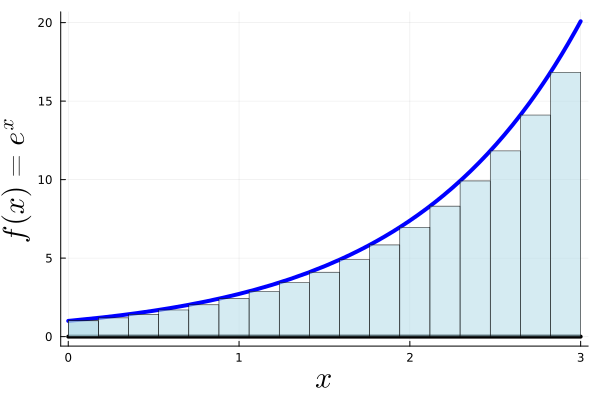
\includegraphics[width=0.45\columnwidth]{graphics/Chap04/AreaExponentialUnderApprox.png}}%
\hspace{5pt}%
\subfloat[]{%
    %\label{fig:MonotonicB}%
	\centering
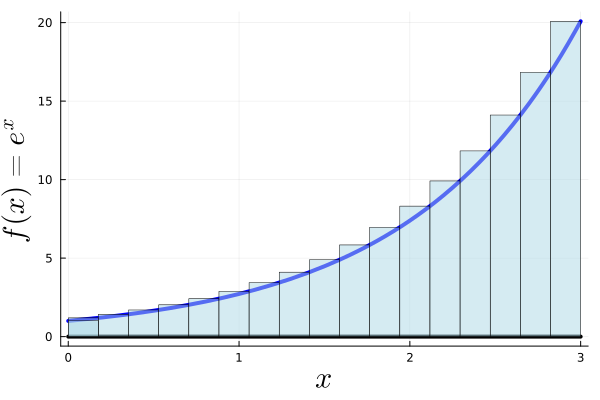
\includegraphics[width=0.45\columnwidth]{graphics/Chap04/AreaExponentialOverApprox.png}}%
    \caption[]{Under- and overapproximations for the area under $e^x$. (a) An underapproximation for the area. (b) An overapproximation for the area.}
    \label{fig:ApproxAreaExponential}
\end{figure}

\subsection{Application to Integrating the Natural Exponential, \texorpdfstring{$e^x$}{ex}}

 \begin{propColor}{Integrating $e^x$}{IntegralExponentialOfx}
For $x>0$ finite, 
 \begin{equation}
 \label{eq:IntegralExpx}
     \int_0^x e^y \, dy = e^x -1.
 \end{equation}
\end{propColor}

\textbf{Proof:} In Chapter~\ref{sec:integratingMonomials}, we developed closed-form expressions for integrating monomials, namely, for $k\in \nat$
$$ \int_0^x y^k dy = \frac{y^{k+1}}{k+1}.$$
 Here, we follow the same pattern to discover the closed-form expression for exponentials, namely,
 \begin{itemize}
     \item Form the Riemann Lower and Upper Sums as indicated in Fig.~\ref{fig:ApproxAreaExponential}.
     \item By taking $\Delta y := \frac{x}{n}$, we will compute lower and upper bounds of \eqref{eq:IntegralExpx}, ${\rm Area}^{\rm Low}_n$ and ${\rm Area}^{\rm Up}_n$, that depend on $n$.
     \item Seek an exact value for \eqref{eq:IntegralExpx} by evaluating $\displaystyle \lim_{n \to \infty} {\rm Area}^{\rm Low}_n$ and $\displaystyle \lim_{n \to \infty} {\rm Area}^{\rm Up}_n$.
     \item If the two limits exist and are equal, then we will have determined the definite integral. 
 \end{itemize}
 \textbf{Let's do it!} \\

We work this out in full detail so as to review the \textbf{Approximation Principle} that undergirds most of Calculus. We let $n>1$ be an integer, and because we are working on the interval $[0, x]$ for $x>0$, we define $\Delta y :=\frac{x-0}{n}$ along with 
$y_i:= a + (i-1) \Delta y$, yielding 
$$ 0 =: a=y_1 < y_2 < \cdots < y_n < y_{n+1} = b:= x.$$
Because $f(y) = e^y$ is increasing, $f(y_i) \le f(y) \le f(y_{i+1})$ for $y \in [y_i, y_{i+1}]$, it is easy to determine the min and max values of the function over subintervals.\\

\textbf{Important Observation:} $e^{k \Delta y} = \left( e^{\Delta y} \right)^k$ by Prop.~\ref{thm:PropertiesExponentials}-(g).\\

\underline{Riemann Lower Sum:}
 We underestimate the total area between $[0, x]$ by summing up the underapproximations, $f(y_i)\cdot \Delta y$, for each interval $[y_i, y_{i+1}]$,
        \begin{equation}
        \begin{aligned}
            {\rm Area}^{\rm Low}_n : =& \sum_{i=1}^n f(y_i)\cdot \Delta y \\
            =& \sum_{i=1}^n e^{(i-1) \Delta y} \cdot \Delta y ~~(\text{substituting in terms})\\
            =&  \sum_{i=1}^n   \left( e^{\Delta y} \right)^{(i-1)}\cdot \Delta y ~~(\text{by the observation})\\
            =& \Delta y\cdot \sum_{i=1}^n   \left( e^{\Delta y} \right)^{(i-1)} ~~(\text{take terms that do not depend on $i$ outside the sum})\\
            =&  \frac{x}{n} \cdot \sum_{i=0}^{n-1}   \left( e^{\Delta y} \right)^{i} ~~(\text{change of index}) \\
            =& \frac{x}{n}\cdot \left( \frac{1 - r^{n}}{1-r}  \right) ~~({\rm Prop}.~\ref{thm:GeometricSums}), 
        \end{aligned}            
        \end{equation}
where
\begin{equation}
    r:=  e^{\Delta y}.
\end{equation}
Hence, after noting that $r^n = e^{n \Delta y} = e^x$, we have
\begin{equation}
  {\rm Area}^{\rm Low}_n  =  \frac{x}{n} \cdot \frac{1 -e^x}{1-e^{ \frac{x}{n}}} = \frac{x}{n} \cdot \frac{e^x - 1}{e^{ \frac{x}{n}} -1}.
\end{equation}
Therefore,
\begin{equation}
\begin{aligned}
  {\rm Area}^{\rm Low} :=& \lim_{n \to \infty} {\rm Area}^{\rm Low}_n  \\
  =&  \lim_{n \to \infty}\frac{x}{n} \cdot \frac{e^x - 1}{e^{ \frac{x}{n}} -1}  \\
  =& \left( e^x - 1 \right) \cdot \lim_{n \to \infty}\frac{x}{n} \cdot \frac{1}{e^{ \frac{x}{n}} -1}  ~~(e^x - 1 ~~~\text{does not depend on n, so factor out of the limit})\\
  =& \left( e^x - 1 \right) \cdot  \lim_{h \to 0^+} h \cdot \frac{1}{e^{ h} -1}  ~~(\text{change of variable}~~ h:= \frac{x}{n} \iff n = \frac{x}{h})\\
  =& \left( e^x - 1 \right) \cdot \lim_{h \to 0^+}  \frac{1}{ \frac{e^{ h} -1}{h}} \\
  =&\left( e^x - 1 \right) \cdot   \frac{1}{\displaystyle \lim_{h \to 0^+} \frac{e^{ h} -1}{h}}  ~~ (\text{by Prop.~\ref{thm:LimitInsideFunction}}) \\
  =& \left( e^x - 1 \right) \cdot \frac{1}{1} \\
  =& e^x-1,
\end{aligned} 
\end{equation}
because, by Example~\ref{ex:KeyExponentialLimit}, $ \displaystyle \lim_{h \to 0^+}  \frac{e^{ h} -1}{h} =1$. Next, we repeat this process for the Riemann Upper Sum\footnote{Because $e^x$ is a continuous function, we know the Riemann integral exists. Hence, the two Riemann sums converge to a common finite value, meaning that we really only have to do one of them to compute the value of the integral. Here, we do both because it is our last opportunity to practice the definition of the Riemann integral!}.\\



\underline{Riemann Upper Sum:} We overestimate the  total area between $[0, x]$ by summing up the overapproximations, $f(y_{i+1})\cdot \Delta y$, for each interval $[y_i, y_{i+1}]$,

        \begin{equation}
        \begin{aligned}
            {\rm Area}^{\rm Up}_n : =& \sum_{i=1}^n f(y_{i+1})\cdot \Delta y \\
            =& \sum_{i=1}^n e^{i \Delta y} \cdot \Delta y ~~(\text{substituting in terms})\\
            =&  \sum_{i=1}^n   \left( e^{\Delta y} \right)^{i}\cdot \Delta y ~~(\text{by the observation})\\
            =& \Delta y\cdot \sum_{i=1}^n   \left( e^{\Delta y} \right)^{i} ~~(\text{take terms that do not depend on $i$ outside the sum})\\
            =&  \frac{x}{n} \cdot \left( \sum_{i=0}^{n}   \left( e^{\Delta y} \right)^{i} -1 \right) ~~(\text{adding and subtracting one for the geometric sum}) \\
            =& \frac{x}{n}\cdot \left( \frac{1 - r^{n+1}}{1-r}   - 1\right) ~~({\rm Prop}.~\ref{thm:GeometricSums}) \\
            =& \frac{x}{n}\cdot r \cdot \left( \frac{r^{n} -1}{r-1} \right) ~~(\text{algebra})
        \end{aligned}            
        \end{equation}
where, as before, $r=  e^{\Delta y} = e^{\frac{x}{n}}$. \\

Hence, after noting that $r^{n} = \left( e^{\Delta y} \right)^n = e^{n \Delta y} = e^x$, we have
\begin{equation}
    {\rm Area}^{\rm Up}_n  =   \frac{x}{n}\cdot e^{ \frac{x}{n}} \cdot \left( \frac{e^x -1}{e^{ \frac{x}{n} }-1}  \right).
\end{equation}
Therefore,
\begin{equation}
\begin{aligned}
  {\rm Area}^{\rm Up} :=& \lim_{n \to \infty} {\rm Area}^{\rm Up}_n  \\
  =&  \lim_{n \to \infty} \frac{x}{n}\cdot e^{ \frac{x}{n}} \cdot \left( \frac{e^x -1}{e^{ \frac{x}{n} }-1}  \right)\\
    =& \left( e^x -1 \right) \cdot \lim_{n \to \infty} \frac{x}{n}\cdot e^{ \frac{x}{n}} \cdot \left( \frac{1}{e^{ \frac{x}{n} }-1}  \right)\\
  =& \left( e^x -1 \right) \cdot \lim_{h \to 0^+} h \cdot e^h \cdot \frac{1}{e^{ h} -1}  ~~(\text{change of variable}~~ h:= \frac{x}{n})\\
  =&\left( e^x -1 \right) \cdot  \lim_{h \to 0^+}  \frac{1}{ \frac{e^{ h} -1}{h}} \cdot \lim_{h \to 0^+} e^h ~~(\text{by Prop.~\ref{thm:LimitInsideFunction}}) \\
  =& \left( e^x-1 \right) \cdot 1 \cdot 1 \\
  =& e^x-1,
\end{aligned}  .
\end{equation}
because, 
\begin{itemize}
    \item by Example~\ref{ex:KeyExponentialLimit}, $ \displaystyle \lim_{h \to 0^+}  \frac{e^{ h} -1}{h} =1$, and
    \item because $e^x$ is continuous, $\displaystyle \lim_{h \to 0^+} e^h = e^{\left( \displaystyle \lim_{h \to 0^+} h \right)} = e^0 = 1$.
\end{itemize}

The limits of the Riemann Lower and Upper Sums both exist and are equal. Hence, our proof is complete.
\Qed

\bigskip


 \begin{propColor}{Integrating $e^{\alpha x}$}{IntegralScaledExponentialOfx}
For $x>0$ finite and $\alpha \in \real$ non-zero,
 \begin{equation}
 \label{eq:IntegralExpAlpahx}
     \int_0^x e^{\alpha y}\, dy = \frac{1}{\alpha} \cdot \left(e^{\alpha x} -1 \right).
 \end{equation}
\end{propColor}

\textbf{Proof:} By Prop.~\ref{thm:IntegralScalingProperty}, Integration and Scaling, 
\begin{align*}
    \int_0^x e^{\alpha y}\, dy &= \frac{1}{\alpha} \int_{\alpha \cdot 0}^{\alpha\cdot x} e^{y} \, dy \\[1em]
    &= \frac{1}{\alpha}  e^y~ \Big|_{\alpha \cdot 0}^{\alpha\cdot x} \\[1em]
    &= \frac{1}{\alpha} \left(e^{\alpha x} -1 \right)
\end{align*}

\Qed

\bigskip

\begin{example} Evaluate the limit as $n\to \infty$ of the finite sum,
$$ \frac{1}{n} \sum_{k=1}^n e^{\frac{k}{n}} = \frac{\sqrt[n]{e^1} + \sqrt[n]{e^2} + \cdots + \sqrt[n]{e^n}}{n}. $$
    
\end{example}

\solution See the video, ``\href{https://www.youtube.com/shorts/d4xpB32bc5Y?feature=share}{the trick you need to know for limits}'', by Michael Penn

\Qed

\begin{factColor}{Euler's Formula for Integrating Sine and Cosine}{EulerSineCosineIntegration} 

Recall that by Euler's formula, 
\begin{equation}
    \begin{aligned}
        \cos(\omega_0 x) &= \frac{e^{\im \omega_0 x}+ e^{-\im \omega_0 x}}{2} \\[1em]
        \sin(\omega_0 x) &= \frac{e^{\im \omega_0 x}- e^{-\im \omega_0 x}}{2 \im}.
    \end{aligned}
\end{equation}

While we have not proved it, Prop.~\ref{thm:IntegralScaledExponentialOfx} also holds for $\alpha \in \cp$ non-zero. Hence,
\begin{equation}
    \begin{aligned}
        \int_0^x e^{\im \omega_0 y} \, dy &= \frac{1}{\im \omega_0} \left( e^{\im \omega_0 x} -1 \right) \\[1em]
        \int_0^x e^{-\im \omega_0 y} \, dy& = \frac{-1}{\im \omega_0} \left(e^{-\im \omega_0 x} -1 \right).
    \end{aligned}
\end{equation}
Hence, after some algebra, we obtain
\begin{equation}
    \begin{aligned}
       \int_0^x \cos(\omega_0 y) \, dy&= \frac{1}{\omega_0}  \sin(\omega_0 x) \\[1em]
       \int_0^x  \sin(\omega_0 y)\, dy &= \frac{1}{\omega_0} \left(1 - \cos(\omega_0 x)  \right).
    \end{aligned}
\end{equation}

We will not belabor this point here because, in Chapter~\ref{chap:AntiDerivFundThmCalc}, we'll find another means to arrive at the same result. Nevertheless, it's pretty cool how things tie together.    
\end{factColor}

\bigskip

\begin{figure}[htb]%
\centering
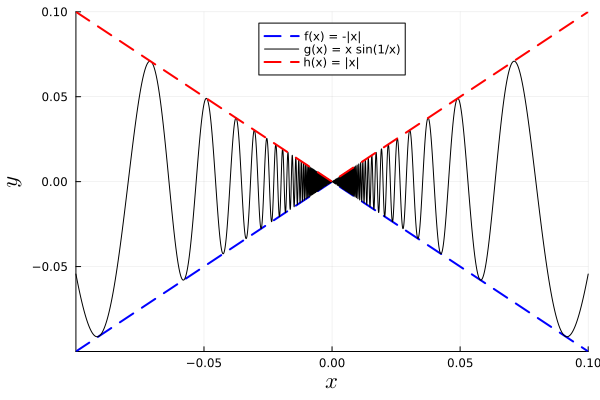
\includegraphics[width=0.7\columnwidth]{graphics/Chap04/SqueezeTheoremPlot.png}%
    \caption[]{\textbf{(Squeeze or Sandwich Theorem:)} If a function is sandwiched between two functions that have a common limit, then the function itself also has the same limit. }
    \label{fig:SqueezeTheorem}
\end{figure}

\section{The Squeeze Theorem}

\begin{propColor}{Squeeze or Sandwich Theorem}{SqueezeTheorem}

Suppose that $a < x_0 < b$ and that \(f\), \(g\), and \(h\) are functions from the interval $(a, b)$ to \(\mathbb{R}\), except possibly being undefined at $x_0$ itself (the usual situation we face when computing limits). If for every $x \in (a, b)$, $x \neq x_0$, it holds that,
\[f(x) \leq g(x) \leq h(x)\]
and if 
\[\lim_{x \to x_0} f(x) = \lim_{x \to x_0} h(x) = L,\]
then 
\[\lim_{x \to x_0} g(x) = L.\]  
\bigskip

\textbf{Note:} The result also holds for limits from the left or right at $x_0$. To see this, simply redefine all three functions to the limit from the left for $x>x_0$ (or the limit from the right, for $x < x_0$). A proof is given in \href{https://en.wikipedia.org/wiki/Squeeze_theorem}{Wikipedia}, which also has some good examples. 
\end{propColor}
\bigskip






\bigskip

\begin{example} 
\label{ex:SqueezeTheorem}
Use the Squeeze Theorem to evaluate the following limits.

\begin{enumerate}
\renewcommand{\labelenumi}{(\alph{enumi})}
\setlength{\itemsep}{.2cm}

    \item $\displaystyle \lim_{x \to 0} x \sin(\frac{1}{x})$.


        \item $\displaystyle \lim_{x \to 0} \frac{\sin(x)}{x}$.

    \item  $\displaystyle \lim_{x \to 0} \frac{1 - \cos(x)}{x}$.
\end{enumerate}
    
\end{example}

\solution 

\begin{enumerate}
\renewcommand{\labelenumi}{(\alph{enumi})}
\setlength{\itemsep}{.2cm}

    \item \Ans~~$\displaystyle \lim_{x \to 0} x \sin(\frac{1}{x}) =0$.\\

    The intuition is illustrated in Fig.~\ref{fig:SqueezeTheorem}. For an analytical proof, because $-1 \le \sin(\frac{1}{x}) \le 1$ for all $x\neq 0$, we have that
    \begin{align*}
        -x \le &x\, \sin(\frac{1}{x}) \le x ~~(\text{multiply both sides by }x>0) \\
         -x \ge &x\, \sin(\frac{1}{x}) \ge x ~~(\text{multiply both sides by } x < 0~\text{and note the flipped inequaliies})
         \\
         x \le &x\, \sin(\frac{1}{x}) \le -x ~~(\text{rewrite the above line from right to left, still for } x < 0).         
    \end{align*}

From the first and last lines, we have
    $$ -|x| \le x \, \sin(\frac{1}{x}) \le|x|, $$
    as illustrated in Fig.~\ref{fig:SqueezeTheorem}. Hence, we can take $f(x):= -|x|$, $g(x):=x\, \sin(\frac{1}{x})$, and $h(x):= |x|$. Because
    $$\lim_{x \to 0}f(x) =  \lim_{x \to 0}h(x) = 0,$$
    the Squeeze Theorem gives the stated conclusion. 


\begin{figure}[hbt]
\centering
\subfloat[]{%
	\centering
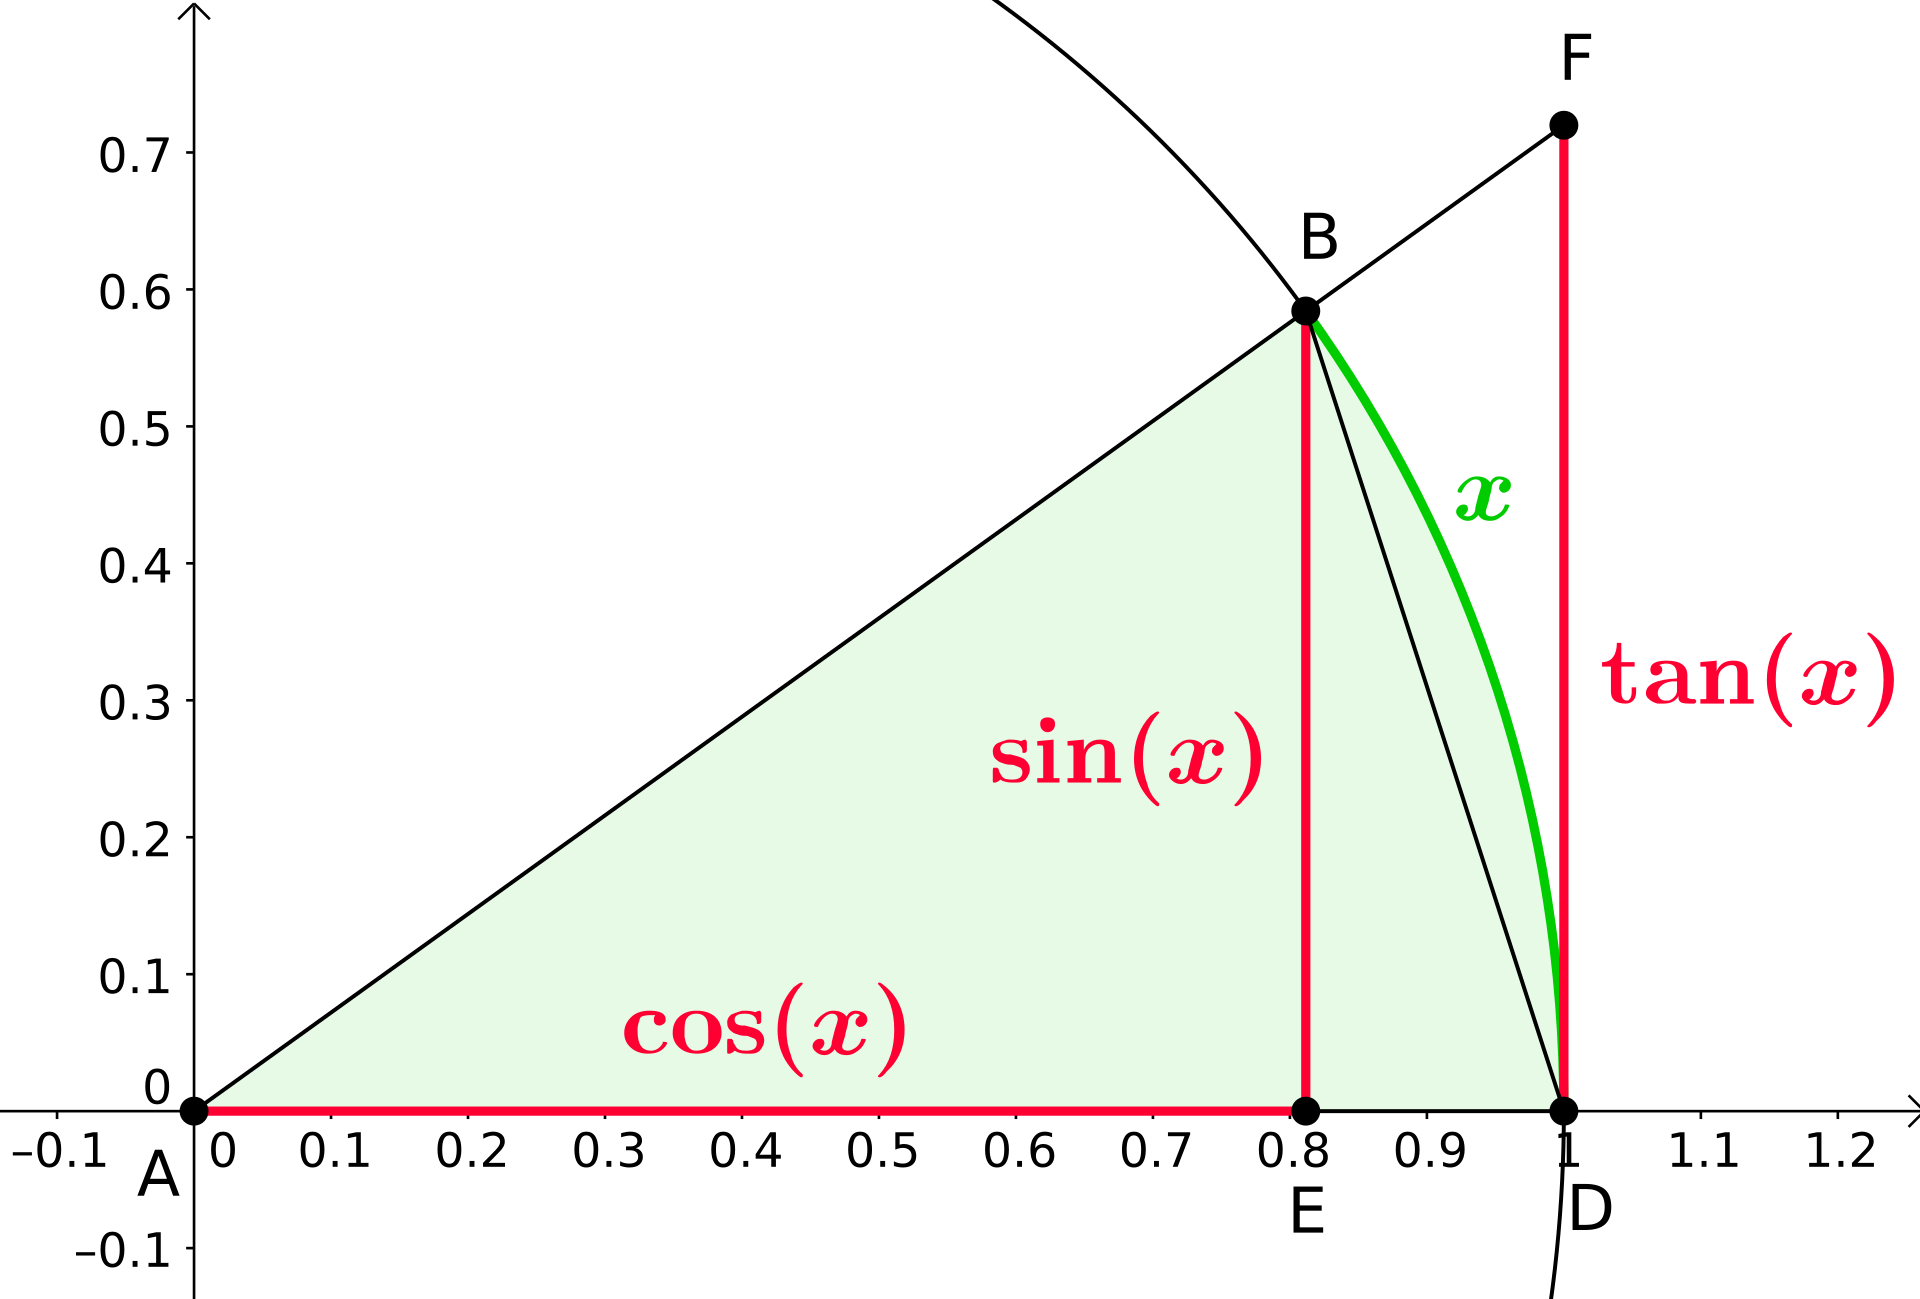
\includegraphics[width=0.45\columnwidth]{graphics/Chap04/TrigFunctionsAndArea.png}}%
\vspace{10pt} % Adds some vertical space between the image and the table
\subfloat[]{%
	\centering
\renewcommand{\arraystretch}{1.8}
\begin{tabular}{|c|c|c|c|c|c|}
\hline
& $Area(\triangle ADB)$ & $\leq$ & $Area(\text{sector } ADB)$ & $\leq$ & $Area(\triangle ADF)$ \\
\hline
$\implies$ & $\frac{1}{2} \cdot \sin(x) \cdot 1$ & $\leq$ & $\frac{x}{2\pi} \cdot \pi$ & $\leq$ & $\frac{1}{2} \cdot \tan(x) \cdot 1$ \\
\hline
$\implies$ & $\sin(x)$ & $\leq$ & $x$ & $\leq$ & $\frac{\sin(x)}{\cos(x)}$ \\
\hline
$\implies$ & $\frac{\cos(x)}{\sin(x)}$ & $\leq$ & $\frac{1}{x}$ & $\leq$ & $\frac{1}{\sin(x)}$ \\
\hline
$\implies$ & $\cos(x)$ & $\leq$ & $\frac{\sin(x)}{x}$ & $\leq$ & $1$ \\
\hline
\end{tabular}
}
\caption{Image and Table from \href{https://en.wikipedia.org/wiki/Squeeze_theorem}{Wikipedia}. The image shows a right triangle $\triangle ADB$, a sector of the unit circle, ${\rm sector} ~ADB$ having perimeter $x$ radians, and a right triangle $\triangle ADF$. The table notes their respective areas and relative sizes. From the formulas for area, useful implications ($\implies$) are obtained for bounding $\sin(x)$ and $\cos(x)$. }
\label{fig:TrigFunctionsAndArea}
\end{figure}


        \item \Ans~~ $\displaystyle \lim_{x \to 0} \frac{\sin(x)}{x} = 1$.\\

        The hard work is done in Fig.~\ref{fig:TrigFunctionsAndArea}, which shows that we can take $f(x):= \cos(x)$, $g(x):=\frac{\sin(x)}{x}$, and $h(x):= 1$. Because
    $$\lim_{x \to 0}f(x) =  \lim_{x \to 0}h(x) = 1,$$
the Squeeze Theorem gives the stated conclusion. 

    \item \Ans ~~ $\displaystyle \lim_{x \to 0} \frac{1 - \cos(x)}{x} = 0$.\\

This is the most challenging problem. For $x>0$,
\begin{equation}
\label{eq:HardBoundingForSqueezeTheoremExample}
    \begin{aligned}
        \cos(x) \le & \frac{\sin(x)}{x} \le 1 \\
       & \Downarrow \\  
               \cos(x) \le & \frac{\sqrt{1 - \cos^2(x)}}{x} \le 1 ~~(\text{Basic trig identity})\\
       & \Downarrow \\  
    \cos^2(x) \le & \frac{1 - \cos^2(x)}{x^2} \le 1 ~~(\text{Square ``all'' sides})\\
       & \Downarrow \\   
          x\,  \cos^2(x) \le & \frac{1 - \cos^2(x)}{x} \le x ~~(\text{Multiply ``all'' sides by } x>0)\\
       & \Downarrow \\ 
        x\,  \cos^2(x) \le & \frac{\left(1 - \cos(x) \right) \left(1 + \cos(x) \right)}{x} \le x ~~(\text{Factor the middle term}).\\  
    \end{aligned}
\end{equation}
\end{enumerate}
Applying the Squeeze Theorem to the last line of \eqref{eq:HardBoundingForSqueezeTheoremExample}, we obtain
$$\lim_{x \to 0+}  \frac{\left(1 - \cos(x) \right) \left(1 + \cos(x) \right)}{x}  = 0.$$
And because $\displaystyle \lim_{x \to 0+} \left(1 + \cos(x) \right) = 1$, it follows that $\lim_{x \to 0+}  \frac{\left(1 - \cos(x) \right) }{x}  = 0$.\\

To complete the problem, we need to compute the limit from the left, which we leave for the learner. The key issue is that we used $x>0$ in the fourth line of 
\eqref{eq:HardBoundingForSqueezeTheoremExample}. When multiplying by $x<0$, the inequalities in that line need to be flipped.
\Qed
\bigskip 


\begin{figure}[htb]%
\centering
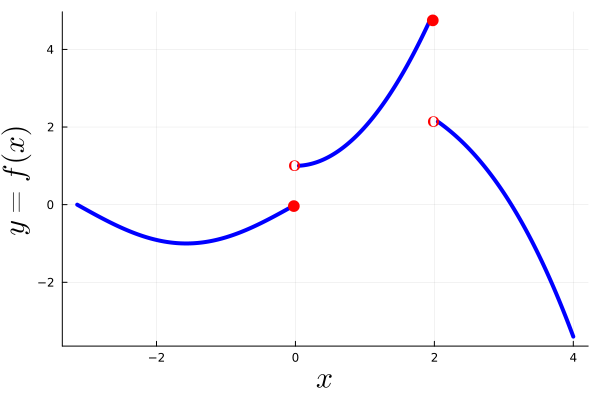
\includegraphics[width=0.4\columnwidth]{graphics/Chap04/PiecewiseExample01.png}%
    \caption[]{The function $f:[-\pi, 4] \to \real$ is an example of what we will call a \textbf{piecewise continuous function}. If we look at the function on the open interval $(-\pi, 0)$,  the function is continuous and has finite one-sided limits at $-\pi$ and 0 (i.e., the two ends of the interval); the function is also continuous on the interval $(0, 2)$ and has finite one-sided limits at $0$ and $2$; finally, the function is continuous on the open interval $(2, 4)$ and has finite one-sided limits at $2$ and $4$.}
    \label{fig:PiecewiseExample01}
\end{figure}

%\clearpag

\section{Piecewise Continuity}

When a function is discontinuous, it may be continuous on subintervals of its domain of definition, as illustrated in Fig.~\ref{fig:PiecewiseExample01}. Such functions occur in Engineering when we are controlling the speed of a robot, for example. When we update a planned speed profile, it is not always convenient to make the command continuous. Allowing for jumps gives us more freedom in directing the robot. 

When we studied definite integrals, we noted that a continuous function on a closed interval $[a, b]$ could always be integrated. We will define piecewise continuous functions in such a way that they can be integrated as well. 

\begin{tcolorbox}[colback=mylightblue, title = {\bf Piecewise Continuity}, breakable]
\begin{definition}
\label{def:piecewiseContinuous}
A real-valued function $f:[a, b] \to  \real$, $a < b $ both finite, is \textbf{piecewise continuous} if there exists a partition of $[a, b]$, 
\begin{equation}
    a=:a_1 < a_2 < \cdots < a_{n+1}:=b,
\end{equation}
such that for all $1 \le i \le n$,
\begin{enumerate}
\renewcommand{\labelenumi}{(\alph{enumi})}
\setlength{\itemsep}{.2cm}
    \item $f(a_i, a_{i+1}) \to \real $ is continuous (i.e., $f$ is continuous on the open interval $(a_i, a_{i+1})$,  
    \item $\displaystyle \lim_{x \to a_i^+} f(x)$ and $\displaystyle \lim_{x \to a_{i+1}^-} f(x)$ both exist and are finite, and
    \item $\displaystyle \lim_{x \to a+} f(x) = f(a)$ and $\displaystyle \lim_{x \to b^-} f(x) = f(b)$ (matches the function definition at the two endpoints).
\end{enumerate}

\bigskip
A function $f:I\to \real$, for $I$ an \textbf{unbounded interval}, is \textbf{piecewise continuous} if for all (bounded) intervals $[a, b] \subset I$, $a < b$ finite,
    $$ \bar{f}:[a, b] \to \real \text{ by } \bar{f}(x) :=f(x) $$
satisfies the above conditions for piecewise continuity. 

\end{definition}
\textbf{Notes:}
\begin{itemize}
    \item We've broken the interval $[a, b]$ into pieces, hence the adjective \textbf{``piecewise''}, and we impose properties on the function for each of the pieces. Since we are defining ``piecewise continuity,'' the condition in (a) is evidently important. What is the role of the two limits in (b)? They prevent the function from ``exploding at the points $a_i$, $2\le i \le n$'' as we will illustrate shortly. You can take a look back at Example~\ref{ex:LimitsTangentOfx} to see what this means! 
    \item What about functions defined on an open interval, $f:(a, b) \to \real$? If the two limits $ \displaystyle \lim_{x \to a+} f(x) $ and $\displaystyle \lim_{x \to b-} f(x) $ exist and are finite, then simply define $f_e :[a, b] \to \real$ by
    $$ f_e(x):= \begin{cases}
         \displaystyle \lim_{x \to a+} f(x) & x = a \\
         \\
          f(x) & a < x < b \\
          \\
         \displaystyle \lim_{x \to b-} f(x) & x = b.
    \end{cases}$$
    You can then apply the definition to the extended function, $f_e$. If one of the two one-sided limits does not exist or is infinite, then the function is automatically not piecewise continuous. 
    \item Some books do not include the requirement that the function has finite limits at the ``boundary points'', $a_i$. We will always require that the two limits exist and are finite, but in other contexts, you have to be careful. 
    \item If $f:[a, b] \to  \real$ is continuous, then it is also piecewise continuous. The converse is evidently false, as exemplified in Fig.~\ref{fig:PiecewiseExample01}.
    \item There is no such thing as ``piecewise continuous at a point.''
    
\end{itemize}
\end{tcolorbox}

\clearpage

\begin{figure}[htb]%
    \centering
\subfloat[]{%
	\centering
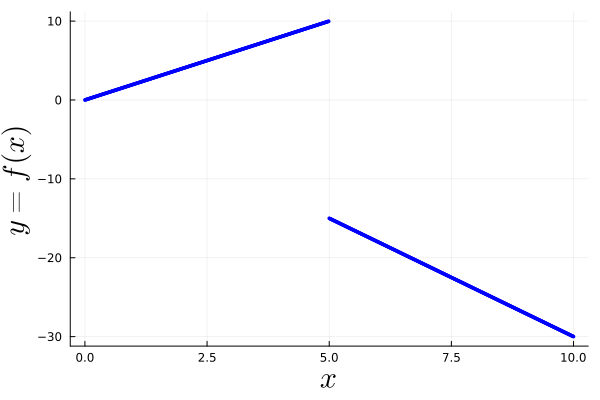
\includegraphics[width=0.45\columnwidth]{graphics/Chap04/PiecewiseContProblemA.png}}%
\hspace{15pt}%
\subfloat[]{%
    %\label{fig:MonotonicB}%
	\centering
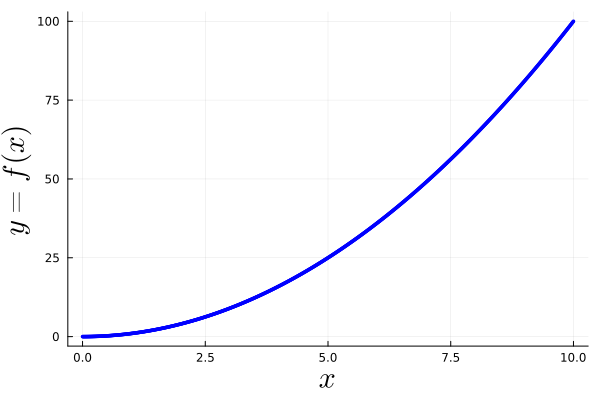
\includegraphics[width=0.45\columnwidth]{graphics/Chap04/PiecewiseContProblemB.png}}%
\newline
\centering
\subfloat[]{%
    %
	\centering
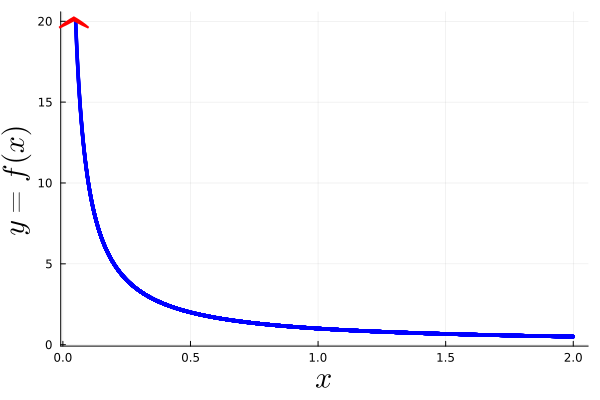
\includegraphics[width=0.45\columnwidth]{graphics/Chap04/PiecewiseContProblemC.png}}%
\hspace{5pt}%
\subfloat[]{%
    %\label{fig:MonotonicB}%
	\centering
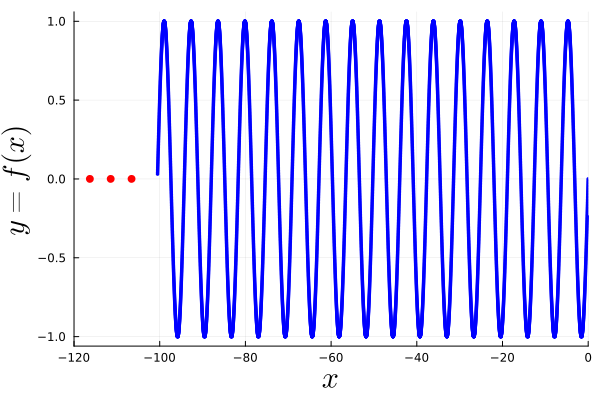
\includegraphics[width=0.45\columnwidth]{graphics/Chap04/PiecewiseContProblemD.png}}%
    \caption[]{Graphs for Example~\ref{ex:WhichArePiecewiseContinuous}. In (c), the graph heads to $\infty$ as $x \to 0^+$. In (d), the graph extends infinitely to the left, oscillating between $-1$ and $+1$ as sine waves like to do! The graphs in (a) and (b) show all the values of the functions.}
    \label{fig:PiecewiseContinuity}
\end{figure}

\bigskip


\begin{example}
\label{ex:WhichArePiecewiseContinuous}
    Determine which, if any, of the following functions are piecewise continuous. 

\begin{enumerate}
\renewcommand{\labelenumi}{(\alph{enumi})}
\setlength{\itemsep}{.2cm}
    \item $f:[0, 10] \to \real$ by $f(x) = \begin{cases}
        2 x & 0 \le x < 5 \\
        -3 x & 5 \le x \le 10
            \end{cases}$.
    \item $f:[0, 10) \to \real$ by $f(x) = x^2$.
    \item  $f:(0, 2] \to \real$ by $f(x) = \frac{1}{x}$.
    \item  $f: (-\infty, 0)  \to \real$ by $f(x) = \sin(x)$.
\end{enumerate}
\end{example}

\textbf{Solutions:} Plots are provided in Fig.~\ref{fig:PiecewiseContinuity}; analytical reasoning is provided below.

\begin{enumerate}
\renewcommand{\labelenumi}{(\alph{enumi})}
\setlength{\itemsep}{.2cm}
    \item \Ans Piecewise continuous.\\ 

    We break the interval $[0, 10]$ into two pieces, $A_1:=(0, 5)$ and $A_2:=(5, 10)$ with
    $$ f_1:(0, 5) \to \real, \text{ by } f_1(x) = 2 x \text{ and } f_2:(5, 10) \to \real, \text{ by } f_2(x) = -3 x.$$
    Each of these functions is continuous and 
    $$\displaystyle \lim_{x \to 0^+} f_1(x) = 0=f(0),  \lim_{x \to 5-} f_1(x) = 10, \lim_{x \to 5+} f_2(x) = -15, \text{ and } \lim_{x \to 10^-} f_2(x) = -30 = f(10).$$
    Hence, all of the conditions are met.

    \item \Ans Piecewise continuous. \\
    
    $f(x) = x^2$ has a finite left limit at $x=10$ and it is equal to $(10)^2$. Therefore, we have $f_e:[0, 10] = x^2$, which we know is continuous everywhere, and hence it is piecewise continuous. 
    
    \item  \Ans Not piecewise continuous because $\displaystyle \lim_{x \to 0^+} \frac{1}{x} = \infty$. Our definition of piecewise continuity requires finite limits.
    
    \item \Ans Piecewise continuous, because
    \begin{itemize}
        \item the function has a finite left limit at zero, namely, $\displaystyle \lim_{x \to 0^-}\sin(x) = 0$, and
        \item the function is continuous everywhere for all bounded intervals $[a, 0)$, for $a < 0$ finite.
    \end{itemize}
   
\end{enumerate}
\Qed

\bigskip

\begin{figure}[htb]%
\centering
\subfloat[]{%
	\centering
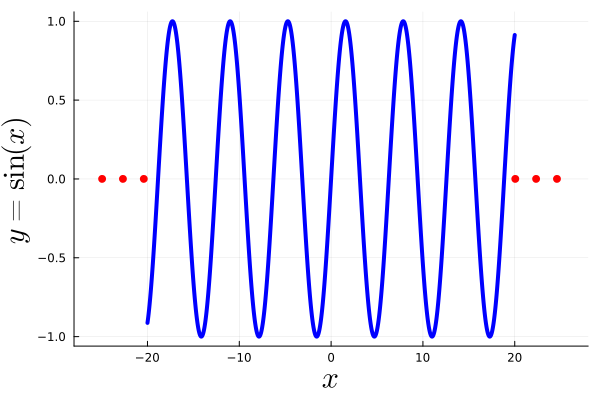
\includegraphics[width=0.4\columnwidth]{graphics/Chap04/BoundsAsymptotesC.png}}%
\hspace{5pt}%
\subfloat[]{%
    %\label{fig:MonotonicB}%
	\centering
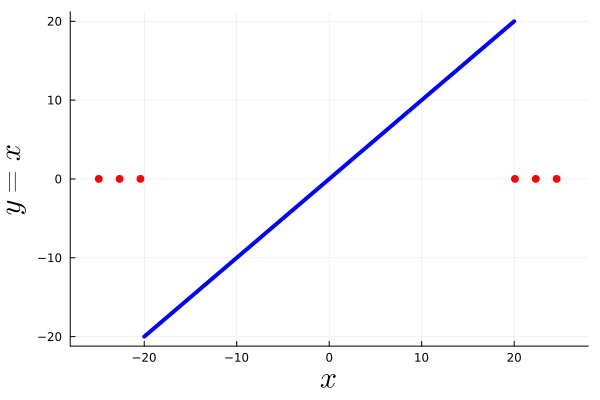
\includegraphics[width=0.4\columnwidth]{graphics/Chap04/BoundsAsymptotesD.png}}%
\newline
\centering
\subfloat[]{%
    %
	\centering
 \hspace{-40pt}%
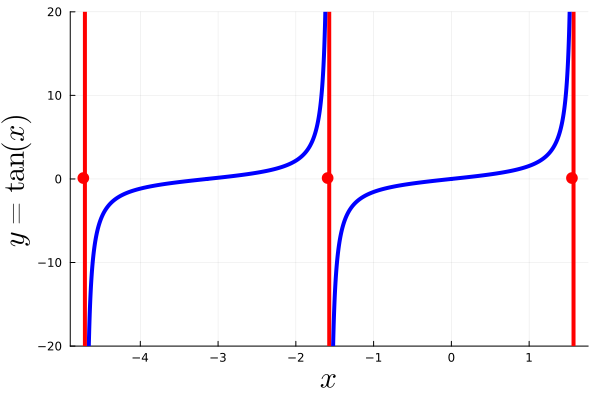
\includegraphics[width=0.4\columnwidth]{graphics/Chap04/BoundsAsymptotesA.png}}%
\hspace{5pt}%
\subfloat[]{%
    %\label{fig:MonotonicB}%
	\centering
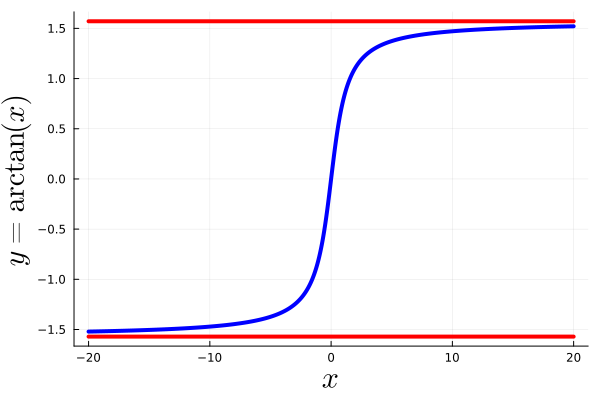
\includegraphics[width=0.4\columnwidth]{graphics/Chap04/BoundsAsymptotesB.png}}%
    \caption[]{Functions can be bounded or unbounded, have horizontal or vertical asymptotes, or not! (a) Bounded, with no asymptotes of any kind. (b) Represents $f(x) = x$ and is unbounded with no asymptotes of any kind (c) Unbounded with vertical asymptotes at odd multiples of $\frac{\pi}{2}$ indicated in red. (d) Bounded with horizontal asymptotes at $\pm \frac{\pi}{2}$ indicated in red}
    \label{fig:BoundedAndAsymptotes}
\end{figure}
\bigskip



\section{Bounded vs Unbounded Functions and Asymptotes}
\label{sec:BoundedFunctions}

Figure~\ref{fig:BoundedAndAsymptotes} illustrates further characteristics of functions that, when present, often aid in their analysis or, in the case of functions of time (aka, trajectories), aid in the analysis of the system that produces them. Bounded functions, such as the sine function, are confined within a fixed range, offering predictability and stability, qualities essential in fields like engineering and physics where maintaining variables within limits is crucial. On the other hand, asymptotes describe the behavior of functions as they approach specific values or infinity, as seen in the tangent and arc-tangent functions. These concepts are not just abstract mathematical ideas but are pivotal in understanding growth rates, stability, and constraints in real-world applications ranging from economic models to biological processes. 

\bigskip

\begin{tcolorbox}[colback=mylightblue, title = {\bf Bounded Functions}, breakable]
\begin{definition}
\label{def:boundedVersusUnbounded}
Let $A\subset \real $ be a subset of $\real$ or $\whole$, and $f:A \to \real$ a function. 
\begin{enumerate}
\renewcommand{\labelenumi}{(\alph{enumi})}
\setlength{\itemsep}{.2cm}
    \item $f$ is \textbf{bounded from above} if there exists $M < \infty$ such that $f(x) \le M$ for all $x \in A$.
    \item $f$ is \textbf{bounded from below} if there exists $M >-\infty$ such that $f(x) \ge M$ for all $x \in A$.
    \item $f$ is \textbf{bounded} if it is both bounded from above and from below. This is equivalent to there exists $M <\infty$ such that $|f(x)| \le M$ for all $x \in A$.
    \item $f$ is \textbf{unbounded} if it is \textbf{not bounded} (that is, either not bounded from above or not bounded from below). This is equivalent to for all $M <\infty$, there $x \in A$, such that $|f(x)| \ge M$. In particular, a function that is bounded from above but not from below is unbounded, and similarly, a function that is bounded from below but not from above is unbounded.
    \item Recall that when $A \subset \nat$, then $a_n:=f(n)$ defines a sequence $\{a_n\}_{n \in A}$.
\end{enumerate}
\end{definition}
\bigskip

\textbf{Illustration:} See Fig.~\ref{fig:BoundedAndAsymptotes}-(a) and (b).

\bigskip

\textbf{Notes:} The notion of ``boundedness'' appears in:
\begin{itemize}    
    \item \textbf{Numerical Methods}: Bounded functions are easier to approximate numerically. For example, numerical integration techniques often rely on the function being bounded to guarantee a certain level of accuracy.
           
    \item \textbf{Stability}: In control theory and engineering, bounded functions are often desirable because they indicate a system's stability. A bounded output in response to a bounded input usually signifies a stable system.
        
    \item \textbf{Optimization}: Bounded functions are often easier to optimize because you can be certain that the optimum lies within a specific range. This is particularly useful in machine learning algorithms.
    
    \item \textbf{Convergence}: In mathematics and computer science, bounded functions are important for analyzing the convergence of sequences and series. 

\end{itemize}

\end{tcolorbox}

\bigskip
Before we dive into examples, it is worthwhile to understand the related notion of \textbf{asymptotes}.
\bigskip


\begin{tcolorbox}[colback=mylightblue, title = {\bf Asymptotes come in two Flavors: Horizontal and Vertical}, breakable]
\begin{definition}
\label{def:AsymptotesHorizontal}
Let $A\subset \real $ be a subset of $\real$ and $f:A \to \real$ a function. A \textbf{horizontal asymptote} is a horizontal line $y = b$ where the function $f$ approaches $b$ as $x$ approaches positive infinity ($\infty$) or negative infinity ($-\infty$). In other symbols, a horizontal line $y = b$ is a \textbf{horizontal asymptote} if at least one of the following two conditions holds:
\begin{enumerate}
    \item $\displaystyle \lim_{{x \to \infty}} f(x) = b$;
    \item $\displaystyle \lim_{{x \to -\infty}} f(x) = b$.
\end{enumerate}

\end{definition}

\bigskip
\textbf{Illustration:} See Fig.~\ref{fig:BoundedAndAsymptotes}-(c) and (d).

\bigskip

\begin{definition}
\label{def:AsymptotesVertical}
Let $A\subset \real $ be a subset of $\real$ and $f:A \to \real$ a function. A \textbf{vertical asymptote} is a vertical line at $x = x_0$ where the function $f$ approaches $\pm \infty$ as $x$ approaches $x_0$ from the left or the right. In other symbols, a vertical line $\{(x_0, y)~|~ y \in \real \}$ is a \textbf{vertical asymptote} if at least one of the following two conditions holds:
\begin{enumerate}
    \item $\displaystyle \lim_{{x \to x_0^+}} f(x) = \pm \infty$ (the limit exists and is unbounded);
    \item $\displaystyle \lim_{{x \to x_0^-}} f(x) = \pm \infty$  (the limit exists and is unbounded).
\end{enumerate}

 \textbf{Note:} At least one of the limits needs to exist for $x_0$ to be a vertical asymptote. As an example, the function $\displaystyle f(x):=\frac{ \sin( \frac{1}{x} ) }{x^2}$ ``blows up'' as $x$ approaches the origin from the left or from the right, but neither limit exists. Hence, $x_0=0$ is not a vertical asymptote.

\end{definition}

\bigskip

\textbf{Notes:} The notion of ``asymptotes'' is useful because:

\begin{itemize}
    \item \textbf{Behavior at Infinity}: Asymptotes help us understand the behavior of functions as points in their domain approach infinity or a finite point. This is crucial in calculus for evaluating limits and integrals.   

    \item \textbf{Graphical Interpretation}: Asymptotes provide a way to graphically represent the behavior of functions, making it easier to visualize and understand their properties.
     
    \item \textbf{Modeling}: In physics, engineering, and economics, asymptotic behavior can model saturation effects. For example, the law of diminishing returns in economics and saturation current in electrical engineering can be modeled using functions with horizontal asymptotes.
    
    \item \textbf{Simplification}: Asymptotic approximations can often simplify complex functions into more manageable forms, making it easier to perform calculations or gain qualitative insights. 
    
\end{itemize}
\end{tcolorbox}


\bigskip

\begin{center}
\setlength{\fboxrule}{2pt}  % Setting the thickness of the border line
   \fbox{ \parbox{0.9\linewidth}{\textcolor{blue}{\bf As illustrated in Fig.~\ref{fig:BoundedAndAsymptotes}, a function can have at most two horizontal asymptotes, while it can have multiple (even infinite in number) vertical asymptotes or none at all. }
}} 
\end{center}

\bigskip

\begin{example}Determine which of the following functions are bounded versus unbounded. Determine also if they have any asymptotes or not.

    \begin{enumerate}
\renewcommand{\labelenumi}{(\alph{enumi})}
\setlength{\itemsep}{.2cm}
    \item  $f:\real \to \real$ by $f(x) = e^{x}$.
    \item  $f:\real \to \real$ by $f(x) = x^2$.
    \item $f:\real \to \real$ by $f(x) = \frac{.001 x^2 + x}{1 + x^2}$.
    \item $f:\real \to \real$ by $f(x) = \begin{cases} \frac{1}{(x-1)(x+1)} & |x| \neq 1\\ 0 & \text{otherwise} \end{cases}$.
    \item $f:\real \to \real$ by $f(x) = \begin{cases} \frac{x-1}{x^2 - 1} & |x| \neq 1\\ 0 & \text{otherwise} \end{cases}$. \textbf{Hint:} Compare to the previous problem.
    \item $f: \nat \to \real$ by $f(n)=(1 - 1/n)^{-n}$. \textbf{Hint:} See Example~\ref{ex:eToPowerxDerivativeNatLogx}-(a).
    \item $f: \nat \to \real$ by $f(n)= \sum_{k=0}^n\frac{1}{k !}$. \textbf{Hint:} See Chapter~\ref{sec:BinomialMeetsEuler}.
    \end{enumerate}
\end{example}

\textbf{Solutions:}

    \begin{enumerate}
\renewcommand{\labelenumi}{(\alph{enumi})}
\setlength{\itemsep}{.2cm}
    \item  \Ans  $f(x) = e^{x}$ is unbounded. It has a horizontal asymptote at $y=0$, corresponding to $\displaystyle \lim_{x \to -\infty} e^{x} = 0$.
    \item  \Ans $f(x) = x^2$ is unbounded and has no asymptotes.
    \item \Ans $f(x) = \frac{-0.001 x^2 + x}{1 + x^2}$ is bounded and has a horizontal asymptote at $y=-10^{-3}$, corresponding to $\displaystyle \lim_{x \to \pm \infty} f(x) = -10^{-3}$.
    
    \item \Ans  $f(x) = \begin{cases} \frac{1}{(x-1)(x+1)} & |x| \neq 1\\ 0 & \text{otherwise} \end{cases}$ is unbounded with two vertical asymptotes. One is at $x_0 = -1$, corresponding to $\displaystyle \lim_{x \to -1^{-}} f(x) = +\infty$ and $\displaystyle \lim_{x \to -1^{+}} f(x) = -\infty$; the other is at $x_0 = +1$, corresponding to $\displaystyle \lim_{x \to 1^{-}} f(x) = -\infty$ and $\displaystyle \lim_{x \to 1^{+}} f(x) = +\infty$. If you plot the function, the answer jumps out at you. Here, we numerically approximate the limits. 

\begin{lstlisting}[language=Julia,style=mystyle]
f(x) = 1/(x^2-1)
del= 1e-5
X0 = [-1, 1]
Data = Array{Float64}(undef, 0, 2)
for k = 1:2
    x=X0[k]-del
    Data = [Data; x f(x)]
    x=X0[k]+del
    Data = [Data; x f(x)]
end
Data
\end{lstlisting}
\textbf{Output} The first two rows are for $x_0 = -1$ and the last two are for $x_0 = 1$.
\begin{verbatim}
4×2 Matrix{Float64}:
 -1.00001   49999.8
 -0.99999  -50000.3
  0.99999  -50000.3
  1.00001   49999.8
\end{verbatim}
    
    \item \Ans $\displaystyle f(x) = \begin{cases} \frac{x-1}{x^2 - 1} & |x| \neq 1\\ 0 & \text{otherwise} \end{cases}$ has a vertical asymptote at $x_0=-1$, but does not have an additional vertical asymptote at $x_0 = 1$ because the ``apparent singularity'' at $+1$ is canceled by the term in the numerator. You can look at the problem in two ways:\\
    
    \textbf{First: } Because $x^2 - 1 = (x-1)(x+1)$, $ \frac{x-1}{x^2 - 1} =  \frac{x-1}{(x-1)(x+1)}= \frac{1}{x+1}$. \\
    
    \textbf{Second: } Numerically approximate the limits as in the previous problem and see what you get! \\
    \begin{lstlisting}[language=Julia,style=mystyle]
f(x) = (x-1)/(x^2-1)
del= 1e-5
X0 = [-1, 1]
Data = Array{Float64}(undef, 0, 2)
for k = 1:2
    x=X0[k]-del
    Data = [Data; x f(x)]
    x=X0[k]+del
    Data = [Data; x f(x)]
end
Data
\end{lstlisting}
\textbf{Output} The first two rows are for $x_0 = -1$ and show that the right and left limits diverge to $\pm \infty$; the last two are for $x_0 = 1$, and indicate that the left and right limits converge to a half.
\begin{verbatim}
4×2 Matrix{Float64}:
 -1.00001  -100000.0
 -0.99999   100000.0
  0.99999        0.500003
  1.00001        0.499998
\end{verbatim}
Hence, $\displaystyle \lim_{x \to 1^{-}} f(x) = 0.5$ and $\displaystyle \lim_{x \to 1^{+}} f(x) = 0.5$. \\

Both methods are valid.

\item \Ans $f: \nat \to \real$ by $f(n)=(1 - 1/n)^{-n}$ has a horizontal asymptote at $e$ because $\displaystyle \lim_{n \to \infty} (1 - 1/n)^{-n} = e$, Euler's number. We computed the limit in Example~\ref{ex:eToPowerxDerivativeNatLogx}-(a). We illustrate the limit in the following plot.

    \begin{center}
    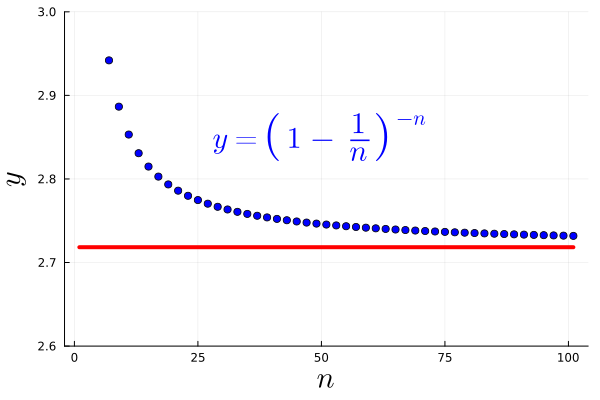
\includegraphics[width=0.45\columnwidth]{graphics/Chap04/BoundsAsymptotesG.png}
    \end{center}

\item \Ans $f: \nat \to \real$ by $f(n)= \sum_{k=0}^n\frac{1}{k !}$ has a horizontal asymptote at $e$. We illustrate this via a plot. Note how fast the summation approaches $e$. Euler really was smart!

    \begin{center}
    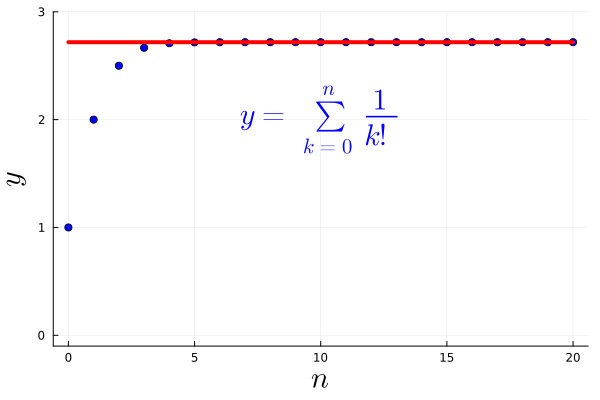
\includegraphics[width=0.45\columnwidth]{graphics/Chap04/BoundsAsymptotesH.png}
    \end{center}
    \end{enumerate}
    \Qed

\section{When does a Function have a Definite Riemann Integral?}
\label{sec:WhenRiemannDefiniteIntegral}

We developed the Riemann Integral in Chapter~\ref{chap:DefiniteIntegration} as the signed area under a curve. Our original development was for continuous functions $f:[a, b] \to \real$, where $[a, b]$ is a closed bounded interval. We now, finally, understand what is a continuous function. We also now understand other properties of functions, such as piecewise continuous functions, bounded functions, and functions that have vertical asymptotes. How do these properties relate to the Riemann Integral? 

\begin{propColor}{Handy List of Functions Having a Riemann Integral}{RiemannIntegrableFuns}

\textbf{Functions Commonly Encountered by Engineers:}
\begin{itemize}
    \item \textbf{Continuous Functions: } All continuous functions on a closed and bounded interval $[a, b]$ are Riemann integrable. This is the most straightforward class of functions that are Riemann integrable. Riemann integrability may fail for continuous functions on an open and bounded interval $(a, b)$ or half-open intervals. It is very important that $a < b$ are finite real numbers and the function is continuous on $[a, b]$.  
    
    \item \textbf{Piecewise Continuous Functions: } A function that is continuous on $[a, b]$ except for a finite number of discontinuities, while having finite left and right limits at the discontinuities, is also Riemann integrable. If the one-sided limits at points of discontinuity either do not exist or are unbounded, then the result can be a function that is not Riemann integrable. Hence, the presence of vertical asymptotes, while not a deal breaker, signals that caution is needed. 
    
    \item \textbf{Bounded Functions with a Finite Number of Discontinuities (not so common, but interesting):}  More generally, any function that is bounded on $[a, b]$ and has a finite number of discontinuities is Riemann integrable. The function doesn't have to be continuous or even piecewise continuous. It does not have to possess one-sided limits at the discontinuities. This result requires graduate-level mathematics to prove. \textit{Mostly, when an engineer encounters such functions, they are piecewise continuous. An example that is not piecewise continuous would be} $f(0):=0$, and for $0 < x < 1$, $f(x) := \sin(1/x)$. The function $f:[0, 1] \to [-1, 1]$ is bounded between $\pm 1$ and has a single discontinuity, namely at $x_0=0$. Amazingly, it is Riemann integrable. 
    
    \item \textbf{Composite Functions:} If $f:[a, b] \to \real$ and $g: [a, b] \to \real$ are both Riemann integrable, then so is $f(g(x))$, provided $f(x)$ is continuous. The function $g$ does not have to be continuous or piecewise continuous. It could be one of the more exotic functions mentioned elsewhere in this list. 

\end{itemize}

\bigskip

\textbf{Functions $f:(a, b) \to \real$ with Vertical Asymptotes or Functions Defined on Unbounded Intervals:}
\begin{itemize}
\item Such integrals are called \textbf{Improper Integrals}, and we treat them in Chapter~\ref{chap:ImproperIntegrals}.
\item Sometimes, we can make sense of them, and sometimes not, as indicated above. 
\item Interesting examples include $\int_0^\infty e^{-x} dx$ (finite), $\int_0^\infty x^k \cdot  e^{-x} dx$ (finite), and $\int_0^1 \frac{1}{x} dx$ (infinite), all of which are encountered frequently. 
\end{itemize}

\bigskip

\textbf{More Exotic Functions, Beyond the Scope of this Course:}
\begin{itemize}
\item \textbf{Monotonic Functions:} Functions that are monotonic (either entirely non-increasing or entirely non-decreasing) on a closed and bounded interval $[a, b]$ are Riemann integrable. \textbf{Such functions could have a countably infinite number of discontinuities and still be Riemann integrable.} For open bounded intervals, $(a, b)$, half-open bounded intervals $[a, b)$ and $(a, b]$, or unbounded intervals, it is NOT true that all monotonic functions are guaranteed to be Riemann integrable. 

\item  \textbf{Functions Equivalent to Continuous Functions:} If a function $f:[a, b] \to \real$ is (i) bounded and (ii) its points of discontinuity have \href{https://en.wikipedia.org/wiki/Lebesgue_measure}{Lebesgue measure} zero, then $f$ is Riemann integrable. Moreover, if (iii), $f$ differs from a continuous function $g: [a, b] \to \real$ on a set of \href{https://en.wikipedia.org/wiki/Lebesgue_measure}{Lebesgue measure} zero, then $f(x)$ is Riemann integrable, and its integral is the same as that of $g(x)$. The Lebesgue measure is treated in graduate-level courses on Functional Analysis or Measure Theory.

\item \textbf{Functions with Bounded Variation:} Functions of \href{https://en.wikipedia.org/wiki/Bounded_variation}{bounded variation} on a closed and bounded interval are \href{https://en.wikipedia.org/wiki/Riemann%E2%80%93Stieltjes_integral}{Riemann-Stieltjes} integrable with respect to any other function of bounded variation. It is noted that the \href{https://en.wikipedia.org/wiki/Lebesgue_integration}{Lebesgue integral} generalizes the Riemann integral and can integrate a broader class of functions. However, every Riemann integrable function is also Lebesgue integrable, and the two integrals will agree on the value for such functions.
\end{itemize}




\end{propColor}

\bigskip



\section{Maximum and Minimum Values of Sets and Their Generalizations}

This is the first time we come close to the ``nitty gritty'' of the real numbers! 

\begin{tcolorbox}[colback=mylightblue, title = {\bf Max and Min Values of a Set}, breakable]
\begin{definition}
\label{def:MaxMinOfSets}
Let $A \subset \real$ be a nonempty subset of the reals.

\begin{enumerate}
\renewcommand{\labelenumi}{(\alph{enumi})}
\setlength{\itemsep}{.2cm}
    \item  $a^\ast$ is a \textbf{maximum element} of the set $A$ if (i) $a^\ast \in A$ and (ii) $a^\ast \ge a$ for all $a \in A$. The notation is
    $$a^\ast = \max\{A\}. $$

    \item  $a_\ast$ is a \textbf{minimum element} of the set $A$ if (i) $a_\ast \in A$ and (ii) $a_\ast \le a$ for all $a \in A$. The notation is
    $$a_\ast = \min\{A\}. $$
\end{enumerate}

\end{definition}
\textbf{Notes:}
\begin{itemize}

    \item A maximum or minimum element must be in the set.  

    \item A finite set always has both maximum and minimum elements. Here, ``finite set'' means a finite number of elements.

   \item A set with an infinite number of elements may not have a maximum or minimum element. 
\end{itemize}
\end{tcolorbox}

\bigskip

\begin{example} Indicate the maximum and minimum elements of the following sets, if they exist.

\begin{enumerate}
\renewcommand{\labelenumi}{(\alph{enumi})}
\setlength{\itemsep}{.2cm}
    \item  $A:=[3, 4]$.

    \item  $B:=(3, 4]$.

    \item  $C:=[3, 4)$.

    \item $D:=(3, 4)$.

    \item $E:= (0, 1) \cap \rat$, the set of rational numbers in the open interval $(0, 1)$.
    
    \item $F:= \{ x\in  [0, 1] ~ | ~ x \notin \rat \}$, the set of irrational numbers in the closed interval $[0, 1]$.
    
\end{enumerate}
    
\end{example}

\textbf{Solutions:}

\begin{enumerate}
\renewcommand{\labelenumi}{(\alph{enumi})}
\setlength{\itemsep}{.2cm}
    \item  \Ans $\min\{A\} = 3$ and  $\max\{A\} = 4$.
    
    While we take this as obvious, you might try writing out a proof by appealing to the definition. It will be good practice. Many proofs in 100- and 200-level math courses boil down to applying the definition to the data at hand.

    \item  \Ans $\min\{B\}$ does not exist while $\max\{B\} = 4$. \\
    
    To prove that the set $B$ does not have a minimum element, let $x \in B$ be arbitrary and define $\delta:=x-3$. Then $\delta >0$ because $3 < x \le 4$. Hence, we have 
    $$3 <  3+\delta/2 < x $$
    and thus $3+\delta/2$ is both smaller than $x$ and an element of $B$; in symbols, $3+\delta/2 < x $ and $(3+\delta/2) \in B$. Hence, $x$ cannot be a minimum, and because $x$ was arbitrary, no element of $B$ can be a minimum.

    \item  \Ans $\max\{C\}$ does not exist while $\min\{C\} = 3$. \\
    
    To prove that the set $C$ does not have a maximum element, let $x \in C$ be arbitrary and define $\delta:=4-x$. Then $\delta >0$ because $4 \notin C$. Hence, we have 
    $$ x < x+\delta/2 < 4 $$
    and thus $x+\delta/2  > x $ and $(x+\delta/2 ) \in C$. Hence, $x$ cannot be a maximum, and because $x$ was arbitrary, no element of $C$ can be a maximum.

    \item \Ans Neither  $\min\{D\}$ nor  $\max\{D\}$ exist. The reasoning is the same as in the previous two parts of this Example.

    \item \Ans Neither  $\min\{E\}$ nor  $\max\{E\}$ exist. \\
    
    Let $r \in E$ be an arbitrary rational number in the open interval $(0, 1)$ and define $\delta:=1-r$. Then $\delta >0$ because $1 \notin E$ and $\delta$ is rational because it is the difference of two rational numbers. Then we have 
    $$ r < r+\delta/2 < 1 $$
    and thus $r+\delta/2   > r$ and $(r+\delta/2  ) \in E$ because $r+\delta/2$ is also rational. Hence, $r$ cannot be a maximum. Similar reasoning shows that $r$ cannot be a minimum.
    
    \item \Ans Neither  $\min\{F\}$ nor  $\max\{F\}$ exist. The reasoning is the same as in the previous part of this Example, because, if $x\in F$ is irrational, then $1-x$, $1-x/2$, and $x/2$ are all irrational numbers belonging to $F$. 
    
\end{enumerate}

\Qed

\bigskip

\begin{tcolorbox}[colback=mylightblue, title = {\bf Sup and Inf Values of a Set}, breakable]
\begin{definition}
\label{def:SupInfOfSets}
Let $A \subset \real$ be a nonempty subset of the reals.

\begin{enumerate}
\renewcommand{\labelenumi}{(\alph{enumi})}
\setlength{\itemsep}{.2cm}
    \item  $a^\ast$ is the \textbf{least upper bound (aka, supremum)} of the set $A$ if (i) $a^\ast \in \real$, (ii) $a^\ast \ge a$ for all $a \in A$, and (iii) if $b\in \real$ satisfies $b \ge a$ for all $a \in A$, then $a^\ast \le b$. The notation is
    $$a^\ast = \sup\{A\}, $$
    where ``sup'' is short for ``supremum''. Note that (ii) says that $a^\ast$ is an \ul{upper bound} and (iii) says that, among all upper bounds, it is the \ul{least upper bound}.

    \item  $a_\ast$ is the \textbf{greatest lower bound (aka, infimum)} of the set $A$ if (i) $a_\ast \in \real$, (ii) $a_\ast \le a$ for all $a \in A$, and (iii) if $b\in \real$ satisfies $b \le a$ for all $a \in A$, then $a_\ast \ge b$. The notation is
    $$a^\ast = \inf\{A\}, $$
    where ``inf'' is short for ``infimum''.  Note that (ii) says that $a_\ast$ is a \ul{lower bound} and (iii) says that, among all lower bounds, it is the \ul{greatest lower bound}.
\end{enumerate}

\end{definition}

\begin{rem} Properties of the infimum and supremum.
\begin{itemize}

    \item  The \textbf{key difference between a maximum or minimum element and the corresponding supremum or infimum element} is where they live! $\max\{A\}$ and $\min\{A\}$ must belong to $A$, whereas $\sup\{A\}$ and $ \inf\{A\}$ belong to $\real$. In fact,
    $$\mathcolor{red}{\bf \sup\{A\} =\max\{A\} \iff \sup\{A\} \in A ~~\textcolor{black}{ and } ~~  \inf\{A\} = \min\{A\} \iff \inf\{A\} \in A}.$$
    
    \item \textcolor{blue}{\bf Every bounded set of real numbers has a supremum and an infimum, whereas we noticed in the previous example many bounded sets of real numbers do not have a maximum or a minimum.}

   \item {\bf The existence of the supremum and the infimum for any bounded set of the reals is actually part of the definition of the real numbers. Michigan's Math 451 digs more deeply into this topic.}

   \item \textcolor{blue}{\bf If a set is unbounded from above, such as $[0, \infty)$, it is common to define the supremum as $\infty$. Similarly, if a set is unbounded from below,  it is common to define the infimum as $-\infty$.} {\bf In this way, all subsets of the reals have an infimum and a supremum.}

\end{itemize}
    
\end{rem}

\end{tcolorbox}

\bigskip

\begin{example} Find the supremum and infimum for the following sets, if they exist. If a supremum or infimum is also a maximum or minimum, indicate that as well.

\begin{enumerate}
\renewcommand{\labelenumi}{(\alph{enumi})}
\setlength{\itemsep}{.2cm}
    \item  $A:=[3, 4]$.

    \item  $B:=(3, 4]$.

    \item  $C:=[3, 4)$.

    \item $D:=(3, 4)$.

    \item $E:= (0, 1) \cap \rat$, the set of rational numbers in the open interval $(0, 1)$.
    
    \item $F:= \{ x\in  \real ~ | ~ x \notin \rat \}$, the set of irrational numbers.
    
\end{enumerate}
    
\end{example}

\textbf{Solutions:}

\begin{enumerate}
\renewcommand{\labelenumi}{(\alph{enumi})}
\setlength{\itemsep}{.2cm}
    \item  \Ans $\inf\{A\} = 3$ and  $\sup\{A\} = 4$. Because  $3 = \inf\{A\} \in A$, it is also a minimum. Similarly, because  $4 = \sup\{A\} \in A$, it is also a maximum.

    \item  \Ans $\inf\{B\} =3$ and $\sup\{B\} = 4$. Because  $3 = \inf\{B\} \notin B$, it is NOT a minimum. However, because  $4 = \sup\{B\} \in B$, it is also a maximum.

    \item  \Ans $\inf\{C\} =3$ and $\sup\{C\} = 4$. Because  $3 = \inf\{C\} \in C$, it is also a minimum. However, because  $4 = \sup\{C\} \notin C$, it is NOT a maximum.

    \item \Ans $\inf\{D\} =3$ and $\sup\{D\} = 4$. Because  $3 = \inf\{D\} \notin D$, it is NOT a minimum. Similarly, because  $4 = \sup\{D\} \notin D$, it is NOT a maximum.

    \item \Ans $\inf\{E\} =0$ and $\sup\{E\} = 1$. Because  $0 = \inf\{E\} \notin E$, it is NOT a minimum. Similarly, because  $1 = \sup\{E\} \notin E$, it is NOT a maximum.
    
    \item \Ans $\inf\{F\} = -\infty$ and  $\sup\{F\} = \infty$. Because  $-\infty= \inf\{F\} \notin F$, it is NOT a minimum. Similarly, because  $\infty = \sup\{F\} \notin F$, it is NOT a maximum. Recall that $\pm \infty$ are \ul{concepts, not real numbers}. 
    
\end{enumerate}

\Qed

\bigskip

\section{Maximum and Minimum Values of Functions and Their Generalizations}
    
In some sense, this material should be super easy: it is a repeat of the previous definitions of max, min, sup, and inf applied to the range of a function! In practice, it seems harder to grasp for most learners. Perhaps this is because the range of a function can be very complicated? In any case, we'll change things up and first present the sup and inf, before moving on to max and min.

\bigskip

\begin{tcolorbox}[colback=mylightblue, title = {\bf Extremal Values of a Function (or a Function's Range)}, breakable]
\begin{definition}
\label{def:SupInftFunctions}
Let $f:A \to \real$ be a function, with its domain $A$ being nonempty. Define $Y:=f(A):=\{y \in \real ~| ~ y=f(x)~~\text{for some } x \in A\}$ to be the \textbf{range} of $f$.

\begin{enumerate}
\renewcommand{\labelenumi}{(\alph{enumi})}
\setlength{\itemsep}{.2cm}
    \item  $f^\ast:= \sup\{Y\}$ is the \textbf{supremum} of the range of $f$, though it is most commonly called the supremum of $f$. The notation is
    $$f^\ast = \sup_{x\in A} f(x), \text{ or } f^\ast =\sup \big\{ \{ y=f(x) ~| ~ x \in A\}  \big\},$$
    which provides good insight: $f^\ast$ is the least upper bound of $f(x)$ as $x$ varies over the entire domain, $A$.

    \item   $f_\ast:= \inf\{Y\}$ is the \textbf{infimum} of the range of $f$, though it is most commonly called the infimum of $f$. The notation is
    $$f_\ast = \inf_{x\in A} f(x), \text{ or } f^\ast =\inf \big\{ \{ y=f(x) ~| ~ x \in A\}  \big\},$$
    which provides good insight: $f_\ast$ is the greatest lower bound of $f(x)$ as $x$ varies over the entire domain, $A$.
\end{enumerate}

\textbf{Recalling that the key difference between sup and max is ``where they live'', we define the max and min of a function as follows.}

\begin{enumerate}
\renewcommand{\labelenumi}{(\alph{enumi})}
\setlength{\itemsep}{.2cm}
\setcounter{enumi}{2} 
    \item  $f^\ast:= \sup\{Y\}$ is the \textbf{maximum of $f$} if $f^\ast \in Y$, that is, there exists $\bar{a} \in A$ such that $f(\bar{a}) = f^\ast$. The notation is
    $$f^\ast = \max_{x\in A} f(x),$$
    which provides good insight: $f^\ast$ is the maximum element of $f(x)$ as $x$ varies over the entire domain, $A$.

    \item  $f_\ast:= \inf\{Y\}$ is the \textbf{minimum of $f$} if $f_\ast \in Y$, that is, there exists $\underbar{a} \in A$ such that $f(\underbar{a}) = f^\ast$. The notation is
    $$f_\ast = \min_{x\in A} f(x),$$
    which provides good insight: $f_\ast$ is the minimum element of $f(x)$ as $x$ varies over the entire domain, $A$.
\end{enumerate}

\end{definition}
\textbf{Notes:}
\begin{itemize}

    \item For the maximum (resp., minimum) of a function to exist, there must be an element in the domain that achieves the maximum (resp., minimum) value of the function. This is not the case of the supremum (resp., infimum).
    
    \item $\displaystyle \sup_{x\in A} f(x)$ and $\displaystyle \inf_{x\in A} f(x)$ always exist, while $\displaystyle  \max_{x\in A} f(x)$ and $\displaystyle \min_{x\in A} f(x)$ sometimes exist, and sometimes do not.
    
\end{itemize}
\end{tcolorbox}

 \bigskip

\begin{propColor}{\href{https://en.wikipedia.org/wiki/Extreme_value_theorem}{Extreme Value Theorem} due to Bolzano-1830}{BolzanoExtremeValueTheorem}

Let $f:[a, b] \to \real$ be a \textbf{continuous function on a closed and bounded interval} $[a, b]$. Then $f$ always achieves its extreme values (aka, maximum and minimum values). In other symbols, there always exist $x^\ast \in [a, b]$ and $x_\ast \in [a, b]$ such that 
$$f(x^\ast) =  \max_{a \in A} f(x) \text{ and } f(x_\ast) =  \min_{a \in A} f(x).$$

\textbf{Notes:} The proof is given in Math 451 and ROB 501; it uses really cool techniques. 
    
\end{propColor}

\bigskip

\begin{example} For the following functions, determine their sup (resp., inf) values, and if they exist, also give the max (resp. min) values.

\begin{enumerate}
\renewcommand{\labelenumi}{(\alph{enumi})}
\setlength{\itemsep}{.2cm}
    \item  $f:(-\infty, \infty) \to \real$ by $f(x) = e^{-x}$.

    \item  $f:[0, 10] \to \real$ by $f(x) = \frac{e^{x}}{x^2 + 1}$. 

    % \item   $f:(-\infty, \infty) \to \real$ by $f(x) = \sinc(x) := \begin{cases} \frac{\sin(x)}{x} & x \neq 0 \\ 1 & x = 0 .\end{cases}$
        
    \item   $f:(-\infty, \infty) \to \real$ by $f(x) = e^{-x^2} \sin(x)$

    \item  $f:[0, \infty) \to \real$ by $f(x) = \frac{2x + 1}{x^2 + 1}$.

    \item  $f:[0, 1] \to \real$ by $f(x) = \frac{\tan(x) - x^3}{x^2 + 2 x \sin(x) + 10}$.
    
\end{enumerate}
    
\end{example}

\textbf{Solutions:}

\begin{enumerate}
\renewcommand{\labelenumi}{(\alph{enumi})}
\setlength{\itemsep}{.2cm}
    \item  \Ans $\displaystyle \inf_{-\infty < x < \infty} e^{-x} = 0$ and $\displaystyle \sup_{-\infty < x < \infty} e^{-x} = \infty$. The min and max of $f$ do not exist.\\

    $e^{-x}$ is strictly monotonically decreasing. Hence, $\displaystyle \inf_{-\infty < x < \infty} e^{-x} = \lim_{x \to \infty} e^{-x} = 0$ and  $\displaystyle \sup_{-\infty < x < \infty} e^{-x} = \lim_{x \to -\infty} e^{-x} = \infty$. You can verify this with a plot, if you wish!

    \item  \Ans   $\displaystyle \min_{x \in [0, 10]} \frac{e^{x}}{x^2 + 1} = 1$ and  $\displaystyle \max_{x \in [0, 10]} \frac{e^{x}}{x^2 + 1} = 218.1$.\\
    
    Because the denominator never vanishes, $f:[0, 10] \to \real$ is a continuous function on the closed and bounded interval, $[0, 10]$. Hence, the max and min values do exist. If the function is strictly monotonically increasing, then the extreme values will be at the endpoints of the interval. We do not know enough Calculus at the moment to check whether or not the function is monotonic, so we'll determine the extreme values numerically. The code below also provides values of $x$ that achieve the max and min of $f$. 

    
    \begin{center}
    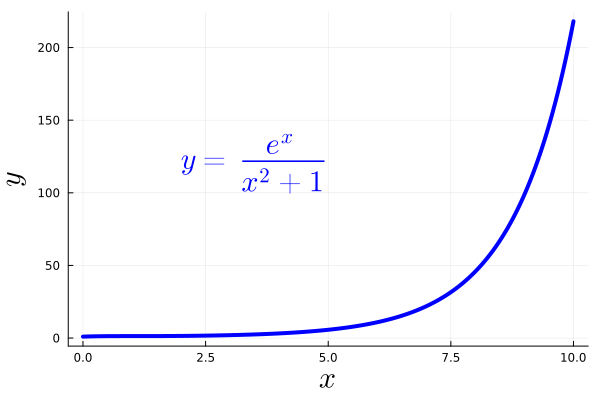
\includegraphics[width=0.45\columnwidth]{graphics/Chap04/MaxMinB.png}
    \end{center}

\begin{lstlisting}[language=Julia,style=mystyle]
xmin = 0
xmax = 10
xVals=xmin:.01:xmax

f(x) = exp(x)/(1 + x^2)

y = f.(xVals)

p1 = plot(xVals,y, linewidth=4, color=:blue, label=false)
plot!(xlabel=L"$x$", ylabel=L"$y=\frac{e^{x}}{x^2 + 1}$") 


@show MaxF = maximum(y)
@show MinF = minimum(y)

max_value, index = findmax(y)
println("Maximum value: ", max_value)
println("x^*: ", xVals[index] )

min_value, index = findmin(y)
println("Minimum value: ", min_value,)
println("x_*: ", xVals[index] )

display(p1)

png(p1, "MaxMinB")
\end{lstlisting}
\textbf{Output} 
\begin{verbatim}
MaxF = maximum(y) = 218.08381975056156
MinF = minimum(y) = 1.0
Maximum value: 218.08381975056156
x^*: 10.0
Minimum value: 1.0
x_*: 0.0
\end{verbatim}

 
\item   \Ans   $\displaystyle \min_{x \in \real} e^{-x^2} \sin(x) = -0.397$ and  $\displaystyle \max_{x \in \real}  e^{-x^2} \sin(x) = 0.397$.\\  
    
    Because the domain of the function is unbounded, Prop.~\ref{thm:BolzanoExtremeValueTheorem} does not apply. \textcolor{red}{\bf However, the function is continuous everywhere on its domain, and it is easy to see that the extreme values do not occur at $\pm \infty$; in fact, they occur within the closed bounded set $[-2, 2]$, where the Proposition does apply}. How did we see all of that? Well, $\displaystyle \lim_{x \to \pm \infty} e^{-x^2} \sin(x) =0$. Yet, we know that $e^{-x^2}$ is always positive, while $\sin(x)$ takes on positive and negative values. Hence, $f(x)$ takes on positive and negative values, and, therefore, the infimum will be negative, and the supremum will be positive. We then need to graph the function to find a range where the extreme values of the function will occur. 

         \begin{center}
    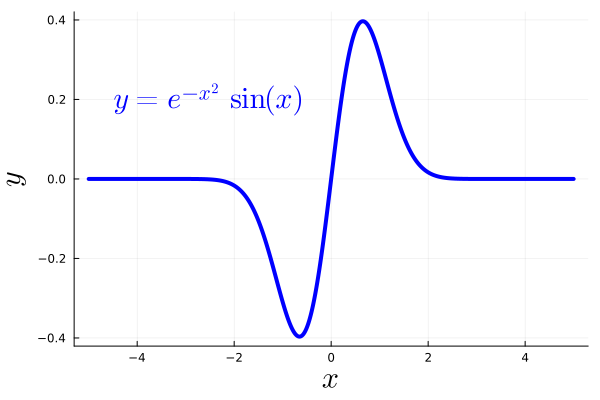
\includegraphics[width=0.45\columnwidth]{graphics/Chap04/MaxMinC.png}
    \end{center}

\begin{lstlisting}[language=Julia,style=mystyle]
xmin = -5
xmax = 5
xVals=xmin:.01:xmax

f(x) = exp(-x^2)*sin(x)

y = f.(xVals)

p1 = plot(xVals,y, linewidth=4, color=:blue, label=false)
plot!(xlabel=L"$x$", ylabel=L"$y=e^{-x^2} ~ \sin(x)$") 

@show MaxF = maximum(y)
@show MinF = minimum(y)

max_value, index = findmax(y)
println("Maximum value: ", max_value)
println("x^*: ", xVals[index] )

min_value, index = findmin(y)
println("Minimum value: ", min_value,)
println("x_*: ", xVals[index] )

display(p1)

png(p1, "MaxMinC")
\end{lstlisting}
\textbf{Output} 
\begin{verbatim}
MaxF = maximum(y) = 0.3966429553529812
MinF = minimum(y) = -0.3966429553529812
Maximum value: 0.3966429553529812
x^*: 0.65
Minimum value: -0.3966429553529812
x_*: -0.65
\end{verbatim}



    
    

    \item  \Ans $\displaystyle \min_{x \in \real} \frac{2x + 1}{x^2 + 1} = 0.423$ and  $\displaystyle \max_{x \in \real} \frac{2x + 1}{x^2 + 1} = 1.618$.\\  
    
    Because the domain of the function is unbounded, Prop.~\ref{thm:BolzanoExtremeValueTheorem} does not apply. \textcolor{red}{\bf However, the function is continuous everywhere on its domain, and it is easy to see that the extreme values do not occur at $\infty$; in fact, they occur within the closed bounded set $[0, 5]$, where the Proposition does apply}. 

    \begin{center}
    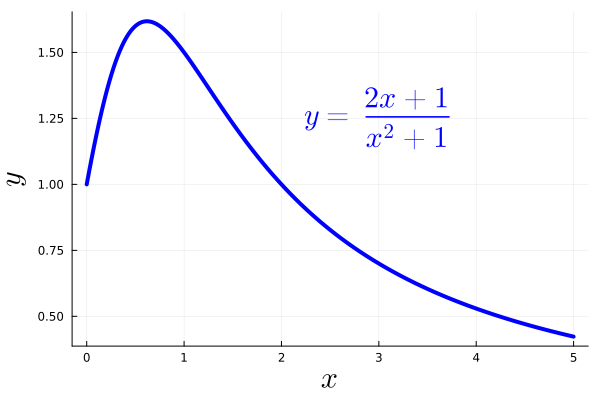
\includegraphics[width=0.45\columnwidth]{graphics/Chap04/MaxMinD.png}
    \end{center}
    
\begin{lstlisting}[language=Julia,style=mystyle]
xmin = 0
xmax = 5
xVals=xmin:.01:xmax

f(x) = (2x + 1)/(x^2 + 1)

y = f.(xVals)

p1 = plot(xVals,y, linewidth=4, color=:blue, label=false)
plot!(xlabel=L"$x$", ylabel=L"$y= \frac{2x + 1}{x^2 + 1}$") 

@show MaxF = maximum(y)
@show MinF = minimum(y)

max_value, index = findmax(y)

println("Maximum value: ", max_value)
println("x^*: ", xVals[index] )

display(p1)

png(p1, "MaxMinD")
\end{lstlisting}
\textbf{Output} 
\begin{verbatim}
MaxF = maximum(y) = 1.6180294712510837
MinF = minimum(y) = 0.4230769230769231
Maximum value: 1.6180294712510837
x^*: 0.62
\end{verbatim}



    \item  \Ans  $\displaystyle \min_{x \in [0, 1]} \frac{\tan(x) - x^3}{x^2 + 2 x \sin(x) + 10} = 0$ and  $\displaystyle \max_{x \in [0, 1]} \frac{\tan(x) - x^3}{x^2 + 2 x \sin(x) + 10} =  0.044$.\\  
    
    Because the denominator never vanishes and $1 < \pi/2$, $f:[0, 1] \to \real$ is a continuous function on the closed and bounded interval, $[0, 1]$. Hence, the max and min values do exist. How do we know the denominator does not vanish? We complete the square,
    $$ x^2 + 2 x \sin(x) + 10 = x^2 + 2 x \sin(x) + 10 + \sin^2(x) -  \sin^2(x) = (x + \sin(x))^2 + 10  -  \sin^2(x),$$
    and we note that, for all $x$, $10-\sin^2(x) \ge 9$ and $ (x + \sin(x))^2 \ge 0$.

    
    \begin{center}
    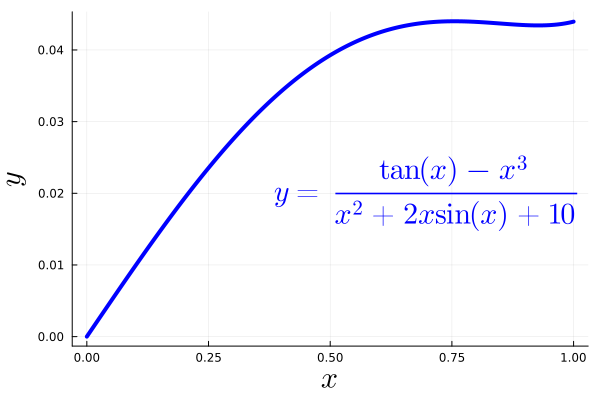
\includegraphics[width=0.45\columnwidth]{graphics/Chap04/MaxMinE.png}
    \end{center}
    
    
\begin{lstlisting}[language=Julia,style=mystyle]
xmin = 0
xmax = 1
xVals=xmin:.001:xmax

f(x) = (tan(x) - x^3)/(x^2 + 2x * sin(x) + 10)

y = f.(xVals)

p1 = plot(xVals,y, linewidth=4, color=:blue, label=false)
plot!(xlabel=L"$x$", ylabel=L"$y= \frac{\tan(x) - x^3}{x^2 + 2 x \sin(x) + 10}$") 

@show MaxF = maximum(y)
@show MinF = minimum(y)

max_value, index = findmax(y)

println("Maximum value: ", max_value)
println("x^*: ", xVals[index] )

display(p1)

png(p1, "MaxMinE")
\end{lstlisting}
\textbf{Output} 
\begin{verbatim}
MaxF = maximum(y) = 0.043999918166140344
MinF = minimum(y) = 0.0
Maximum value: 0.043999918166140344
x^*: 0.755
\end{verbatim}

\end{enumerate}


\Qed

\bigskip

\section{(Optional Read:) Intermediate Value Theorem and the Mean Value Theorem}
\label{sec:AdditionalResultsChap04}

The Intermediate Value Theorem is a fundamental result in calculus and real analysis. It asserts that for any continuous function defined on a closed interval, the function takes on every value between its minimum and maximum on that interval. This theorem has important implications in various areas of mathematics and its applications. We used it to establish the soundness of the Bisection Algorithm.

\bigskip

\begin{propColor}{Intermediate Value Theorem }{IntermediateValueTheorem } Let \( f: [a, b] \to \mathbb{R} \) be a continuous function on the closed interval \([a, b]\), where \( a < b \). If \( d \) is any number between \( f(a) \) and \( f(b) \), then there exists at least one \( c \in [a, b] \) such that \( f(c) = d \).
    
\end{propColor}

\textbf{Proof:} Without loss of generality, assume \( f(a) < d < f(b) \). Define the set \( S = \{ x \in [a, b] \mid f(x) \leq d \} \). \\

Because \( f(a) \leq d \), we have that $a \in S$, and hence the set \( S \) is non-empty. Moreover, the set \( S \) is bounded above by \( b \) because \( S \subset [a, b] \). Finally, by the completeness property of the real numbers, \( S \) has a supremum. Define
$$ c := \sup S. $$

We now want to show that  \( f(c) = d \). Because \( c = \sup S \) and \( c \in [a, b] \), \( c \) is the least upper bound of \( S \). Therefore, for any \( \epsilon > 0 \), there exists an \( x \in S \) such that \( c - \epsilon < x \leq c \).
\begin{itemize}
    \item Since \( x \in S \), \( f(x) \leq d \). Given \( f \) is continuous, we have \( \lim_{x \to c^-} f(x) = f(c) \leq d \).
    \item By definition of \( c \) being the supremum, for any \( \epsilon > 0 \), there exists a point \( y \in [c, c + \epsilon] \) such that \( y \notin S \). Thus, \( f(y) > d \).
    \item Since \( f \) is continuous at \( c \), we have \( \lim_{y \to c^+} f(y) = f(c) \geq d \).
\end{itemize}
Combining these limits, we obtain \( f(c) = d \), and hence, there exists at least one \( c \in [a, b] \) such that \( f(c) = d \).

\Qed


\bigskip

The Mean Value Theorem is a central result in calculus and real analysis. It states that for any function continuous on a closed interval and differentiable on the open interval, there exists at least one point in the open interval where the derivative of the function equals the average rate of change over the closed interval. 

\bigskip


\begin{propColor}{Mean Value Theorem}{MeanValueTheorem}
    Let \( f: [a, b] \to \mathbb{R} \) be a continuous function on the closed interval \([a, b]\) and differentiable on the open interval \((a, b)\), where \( a < b \). Then, there exists at least one \( c \in (a, b) \) such that
    \[
    f'(c) = \frac{f(b) - f(a)}{b - a}.
    \]
\end{propColor}

\textbf{Proof:} Define the function \( g(x) = f(x) - \frac{f(b) - f(a)}{b - a}(x - a) \). Note that \( g \) is continuous on \([a, b]\) and differentiable on \((a, b)\).

We first observe that:
\[
g(a) = f(a) - \frac{f(b) - f(a)}{b - a}(a - a) = f(a),
\]
and
\[
g(b) = f(b) - \frac{f(b) - f(a)}{b - a}(b - a) = f(b) - (f(b) - f(a)) = f(a).
\]

Thus, \( g(a) = g(b) \). By \href{https://en.wikipedia.org/wiki/Rolle%27s_theorem}{Rolle's Theorem}, since \( g \) is continuous on \([a, b]\), differentiable on \((a, b)\), and \( g(a) = g(b) \), there exists at least one \( c \in (a, b) \) such that \( g'(c) = 0 \). Next, we compute \( g'(x) \):
\[
g'(x) = f'(x) - \frac{f(b) - f(a)}{b - a}.
\]

At \( x = c \), we have \( g'(c) = 0 \), which gives us:
\[
f'(c) - \frac{f(b) - f(a)}{b - a} = 0,
\]
or equivalently,
\[
f'(c) = \frac{f(b) - f(a)}{b - a}.
\]

Thus, there exists at least one \( c \in (a, b) \) such that
\[
f'(c) = \frac{f(b) - f(a)}{b - a}.
\]
\Qed

\textbf{Related Videos:}
\begin{itemize}
    \item \href{https://www.youtube.com/watch?v=4L9ffuwj4Lk}{Intermediate Value Theorem} by The Organic Chemistry Tutor

    \item \href{https://www.youtube.com/shorts/EnVN3_lbsGQ}{Mean Value Theorem} by 
@MindSphereYT.
\end{itemize}


\section{(Optional Read:) Proofs Associated with the Chapter}
\label{sec:ProofsChap04}

\bigskip

We first state and prove a few lemmas, and then we get into the proofs. \\

\emstat{

\textbf{Lemma (Product of Two Continuous Functions is Continuous):}  
 Let \(f: [a, b] \rightarrow \mathbb{R}\) and \(g: [a, b] \rightarrow \mathbb{R}\) be continuous functions at a point \(x_0 \in [a, b]\). Then, the function \(h(x) := f(x)g(x)\) is also continuous at \(x_0\).
 }

\textbf{Proof:} To prove that \(h(x)\) is continuous at \(x_0\), we need to show that for every \(\epsilon > 0\), there exists a \(\delta > 0\) such that if \(|x - x_0| < \delta\), then \(|h(x) - h(x_0)| < \epsilon\).\\

Because \(f\) and \(g\) are continuous at \(x_0\), for any \(\epsilon_1 > 0\), there exists \(\delta_1 > 0\) such that if \(|x - x_0| < \delta_1\), then \(|f(x) - f(x_0)| < \epsilon_1\). Similarly, for any \(\epsilon_2 > 0\), there exists \(\delta_2 > 0\) such that if \(|x - x_0| < \delta_2\), then \(|g(x) - g(x_0)| < \epsilon_2\).\\

Let \(\epsilon > 0\). Choose \(\displaystyle \epsilon_1 = \frac{\epsilon}{2(|g(x_0)|+1)}\) and \(\displaystyle \epsilon_2 = \frac{\epsilon}{2(|f(x_0)|+1)}\). By the continuity of \(f\) and \(g\), there exist \(\delta_1\) and \(\delta_2\) corresponding to \(\epsilon_1\) and \(\epsilon_2\), respectively. Let \(\delta = \min\{\delta_1, \delta_2\}\). Then, for \(|x - x_0| < \delta\), we have,
\begin{align*}
|f(x)g(x) - f(x_0)g(x_0)| &= |f(x)g(x) - f(x)g(x_0) + f(x)g(x_0) - f(x_0)g(x_0)| \\
&\leq |f(x)||g(x) - g(x_0)| + |g(x_0)||f(x) - f(x_0)| \\
&< |f(x)|\epsilon_2 + |g(x_0)|\epsilon_1 \\
&\leq (|f(x_0)|+1)\epsilon_2 + (|g(x_0)|+1)\epsilon_1 \\
&= \frac{\epsilon}{2} + \frac{\epsilon}{2} \\
&= \epsilon.
\end{align*}
Therefore, \(h(x) = f(x)g(x)\) is continuous at \(x_0\). 
\Qed
\bigskip

\emstat{\textbf{Lemma (Sum of Two Continuous Functions is Continuous):} Let \(f: [a, b] \to \mathbb{R}\) and \(g: [a, b] \to \mathbb{R}\) be continuous functions on the interval \([a, b]\). Then, the function \(h(x) := f(x) + g(x)\) is also continuous on \([a, b]\).}

\textbf{Proof:} To prove that \(h(x)\) is continuous on \([a, b]\), we need to show that for every point \(x_0 \in [a, b]\) and for every \(\epsilon > 0\), there exists a \(\delta > 0\) such that if \(|x - x_0| < \delta\), then \(|h(x) - h(x_0)| < \epsilon\).\\

Since \(f\) and \(g\) are continuous at \(x_0\), for any \(\epsilon > 0\), there exist \(\delta_f > 0\) and \(\delta_g > 0\) such that:
\begin{itemize}
    \item If \(|x - x_0| < \delta_f\), then \(|f(x) - f(x_0)| < \frac{\epsilon}{2}\).
    \item If \(|x - x_0| < \delta_g\), then \(|g(x) - g(x_0)| < \frac{\epsilon}{2}\).
\end{itemize}

Let \(\delta = \min\{\delta_f, \delta_g\}\). Now, for \(|x - x_0| < \delta\), we have by the triangle inequality,
\begin{align*}
|h(x) - h(x_0)| &= |(f(x) + g(x)) - (f(x_0) + g(x_0))| \\
&= |(f(x) - f(x_0)) + (g(x) - g(x_0))| \\
&\leq |f(x) - f(x_0)| + |g(x) - g(x_0)| \\
&< \frac{\epsilon}{2} + \frac{\epsilon}{2} \\
&= \epsilon.
\end{align*}
Thus, \(h(x) = f(x) + g(x)\) is continuous at \(x_0\). Since \(x_0\) was arbitrary, \(h(x)\) is continuous on the entire interval \([a, b]\). 
\Qed.

\bigskip



\emstat{\textbf{Lemma (Composition of Two Continuous Functions is Continuous):} Let $f: X \rightarrow Y$ and $g: Y \rightarrow Z$ be continuous functions, where $X$, $Y$, and $Z$ are subsets of $\mathbb{R}$. Then, the composition $g \circ f: X \rightarrow Z$, defined by $(g \circ f)(x) := g(f(x))$, is continuous.}

\textbf{Proof:}

To show that $g \circ f$ is continuous at any point $x_0 \in X$, we need to verify that for every $\varepsilon > 0$, there exists a $\delta > 0$ such that if $|x - x_0| < \delta$, then $|(g \circ f)(x) - (g \circ f)(x_0)| < \varepsilon$.\\

Because $g$ is continuous at $f(x_0) \in Y$, for every $\varepsilon > 0$, there exists an $\eta > 0$ such that if $|y - f(x_0)| < \eta$, then $|g(y) - g(f(x_0))| < \varepsilon$, where $y = f(x)$.  Furthermore, since $f$ is continuous at $x_0$, for the $\eta > 0$ found above, there exists a $\delta > 0$ such that if $|x - x_0| < \delta$, then $|f(x) - f(x_0)| < \eta$.\\

Combining these two observations, if $|x - x_0| < \delta$, then $|f(x) - f(x_0)| < \eta$, which implies $|g(f(x)) - g(f(x_0))| < \varepsilon$. This means that $|(g \circ f)(x) - (g \circ f)(x_0)| < \varepsilon$.  Therefore, by the $\varepsilon$-$\delta$ definition of continuity, $g \circ f$ is continuous at $x_0$. Since $x_0$ was arbitrary, $g \circ f$ is continuous on $X$. 
\Qed


\bigskip
\emstat{\bf We leave unproven that all three of these results can be extended to $\bm{n>2}$ functions. You may wish to prove at least one of them for yourself. Each of the extensions can be proven by induction.}


\bigskip




\begin{tcolorbox}[title=\textcolor{black}{Proof of Prop.~\ref{thm:CommonContFuns} (Common Continuous Functions}, sharp corners, colback=green!30, colframe=green!80!blue, breakable, fonttitle=\bfseries]

We'll prove a few of the dozen or more functions listed in Prop.~\ref{thm:CommonContFuns}: the following functions are continuous for all $x\in \real$ \textcolor{blue}{unless indicated otherwise}:

\begin{enumerate}
\renewcommand{\labelenumi}{(\alph{enumi})}
\setlength{\itemsep}{.2cm}
\item Monomials: $f(x) = x^k$

  \item Polynomials: $ f(x) = a_nx^n + a_{n-1}x^{n-1} + \cdots + a_1x + a_0 $
\item  Sine: $ f(x) = \sin(x) $


\item Natural Exponential: $ f(x) = e^x $

\item Natural Logarithm \textcolor{blue}{(continuous for $ x > 0 $)}: $ f(x) = \ln(x) $
  
\item Power \textcolor{blue}{(continuous for $x > 0$ and $y \in \real)$}: $ f(x) = x^y $



  \item Square Root \textcolor{blue}{(continuous for $ x \geq 0 $)}: $ f(x) = \sqrt{x} $

\end{enumerate}

\end{tcolorbox}



\bigskip


\begin{enumerate}
\renewcommand{\labelenumi}{(\alph{enumi})}
\setlength{\itemsep}{.2cm}
\item Monomials: $f(x) = x^k$. \\

We prove by induction that the function $f(x) = x^k$ is continuous for all positive integers $k$.

\textbf{Base Cases:}
\begin{itemize}
    \item For $k=0$, $f(x) = x^0 = 1$, a constant function, which is continuous everywhere.
    \item For $k=1$, $f(x) = x$, the identity function, which is also continuous everywhere.
\end{itemize}

\textbf{Inductive Step:}
Assume $f(x) = x^k$ is continuous. We need to show that $f(x) = x^{k+1}$ is also continuous. Given $f(x) = x^k$ is continuous by our inductive hypothesis, and knowing that $g(x) = x$ is continuous, consider $h(x) := x^{k+1} = x^k \cdot x$. Since the product of two continuous functions is continuous, it follows that $x^{k+1}$ is continuous.\\

Therefore, by mathematical induction, $f(x) = x^k$ is continuous for all positive integers $k$.
\Qed

  \item Polynomials: $ f(x) = a_nx^n + a_{n-1}x^{n-1} + \cdots + a_1x + a_0 $\\

  This follows immediately by the above result for monomials and the lemma on the sum of continuous functions.

  
\item  Sine: $ f(x) = \sin(x) $ \\

To prove continuity at $x_0 \in \real$, we need to show that for every $\epsilon > 0$, there exists a $\delta > 0$ such that if $|x - x_0| < \delta$, then $|\sin(x) - \sin(x_0)| < \epsilon$.\\

Using the trigonometric identity for the difference of two sines, 
\[
|\sin(x) - \sin(x_0)| = |2 \cos\left(\frac{x + x_0}{2}\right) \sin\left(\frac{x - x_0}{2}\right)|.
\]
Because $|\cos(\theta)| \leq 1$ for all $\theta$, and $|\sin(\theta)| \leq |\theta|$ for all $\theta$, we can further simplify the inequality to:
\[
|\sin(x) - \sin(x_0)| \leq |2 \sin\left(\frac{x - x_0}{2}\right)| \leq |x - x_0|.
\]
To ensure $|\sin(x) - \sin(x_0)| < \epsilon$, it suffices to choose $\delta = \epsilon$. Thus, for $|x - x_0| < \delta$, we indeed have $|\sin(x) - \sin(x_0)| < \epsilon$.\\

Therefore, by the $\epsilon$-$\delta$ criterion of continuity, $f(x) = \sin(x)$ is continuous at $x_0$. 
\Qed



  \item Natural Exponential: $ f(x) = e^x $\\

Let $x_0$ be an arbitrary point in $\mathbb{R}$. To prove that $f(x) = e^x$ is continuous at $x_0$, consider any $\varepsilon > 0$. We aim to show that there exists a $\delta > 0$ such that if $|x - x_0| < \delta$, then $|e^x - e^{x_0}| < \varepsilon$.

Given $\varepsilon > 0$, define $\theta > 1$ such that
\[
e^{x_0} - \varepsilon < \frac{e^{x_0}}{\theta} < e^{x_0} < \theta e^{x_0} < e^{x_0} + \varepsilon.
\]
It follows from the definition of $\theta$ that
\[
\frac{e^{x_0}}{\theta} < e^{x_0} < \theta e^{x_0},
\]
which simplifies to
\[
-\ln(\theta) < x - x_0 < \ln(\theta).
\]

Let $\delta = \ln(\theta)$. Then, for $x \in (x_0 - \delta, x_0 + \delta)$, we have
\[
e^{x_0 - \delta} < e^x < e^{x_0 + \delta}.
\]

This implies
\[
\frac{e^{x_0}}{\theta} < e^x < \theta e^{x_0},
\]
or equivalently,
\[
e^{x_0} - \varepsilon < e^x < e^{x_0} + \varepsilon.
\]

Therefore, $|e^x - e^{x_0}| < \varepsilon$ whenever $|x - x_0| < \delta$, proving that $f(x) = e^x$ is continuous at $x_0$. Since $x_0$ was arbitrary, $f(x) = e^x$ is continuous for all $x_0 \in \mathbb{R}$. 
\Qed


  \item Natural Logarithm \textcolor{blue}{(continuous for $ x > 0 $)}: $ f(x) = \ln(x) $\\

Let $x_0 > 0$ be an arbitrary point. To prove that $f(x) = \ln(x)$ is continuous at $x_0$, consider any $\varepsilon > 0$. We must show that there exists a $\delta > 0$ such that if $|x - x_0| < \delta$, then $|\ln(x) - \ln(x_0)| < \varepsilon$.\\

Given $\varepsilon > 0$, consider the intervals $(e^{-\varepsilon}x_0, e^{\varepsilon}x_0)$. For $x$ in this interval, we have $e^{-\varepsilon} < \frac{x}{x_0} < e^{\varepsilon}$, implying that $-\varepsilon < \ln\left(\frac{x}{x_0}\right) < \varepsilon$, which simplifies to $-\varepsilon < \ln(x) - \ln(x_0) < \varepsilon$, or equivalently, $|\ln(x) - \ln(x_0)| < \varepsilon$.\\

Let $\delta = \min\{x_0 - e^{-\varepsilon}x_0, e^{\varepsilon}x_0 - x_0\}$. Then, for $|x - x_0| < \delta$, $x$ lies within the interval $(e^{-\varepsilon}x_0, e^{\varepsilon}x_0)$, ensuring that $|\ln(x) - \ln(x_0)| < \varepsilon$. Therefore, by the $\varepsilon$-$\delta$ definition of continuity, $f(x) = \ln(x)$ is continuous at $x_0$. Since $x_0$ was arbitrary and $x_0 > 0$, $f(x) = \ln(x)$ is continuous for all $x_0 > 0$. 
\Qed


\item Power \textcolor{blue}{(continuous for $x > 0$ and $y \in \real)$}: $ f(x) = x^y $\\

For $x > 0$ and logarithm properties, we have that $x^y= e^{y \ln x}$, which is the composition of the continuous functions, $e^x$ and $y \ln x$.
\Qed

\item Square Root \textcolor{blue}{(continuous for $ x \geq 0 $)}: $ f(x) = \sqrt{x} $\\

  This is a special case of the power function, with $y=\frac{1}{2}$.
  \Qed

\end{enumerate}

\bigskip

    \begin{tcolorbox}[title= \textcolor{black}{Proof of Prop.~\ref{thm:LimitInsideFunction} (Taking Limits Inside a Function)}, sharp corners, colback=green!30, colframe=green!80!blue, breakable, fonttitle=\bfseries]
    
    Consider two functions $g:X \to Y$ and $f:Y \to Z$, where $X$, $Y$, and $Z$ are subsets of $\real$. Suppose that $f$ is continuous at a point $y_0 \in Y$. Then, the following hold:
\begin{enumerate}
\renewcommand{\labelenumi}{(\alph{enumi})}
\setlength{\itemsep}{.2cm}

\item If $x_0 \in \real$ and $\displaystyle \lim_{x \to x_0} g(x) = y_0$ (i.e., the limit exists and equals $y_0$), then $\displaystyle \lim_{x \to x_0} f(g(x)) = f(\lim_{x \to x_0} g(x)) = f(y_0). $ \textbf{We say the limit can be taken ``inside'' the function $f$.}

\item Similarly, if $\displaystyle \lim_{x \to \infty} g(x) = y_0$, then $\displaystyle \lim_{x \to \infty} f(g(x)) = f(\lim_{x \to \infty} g(x)) = f(y_0). $  

\item If $\displaystyle \lim_{x \to -\infty} g(x) = y_0$, then $\displaystyle \lim_{x \to -\infty} f(g(x)) = f(\lim_{x \to -\infty} g(x)) = f(y_0). $ 
\end{enumerate}
In short, if $g(x)$ has a limit (as $x$ approaches a finite point or as $x$ approaches $\pm \infty$), and $f$ is continuous at the limit of $g$ (i.e., $y_0$), then, when evaluating a limit of $f(g(x)) = f\circ g(x)$,  the limit can be taken inside the function $f$ and applied directly to $g$.  
\end{tcolorbox}

\bigskip
\textbf{ Proof:}

\begin{enumerate}
    \renewcommand{\labelenumi}{(\alph{enumi})}
    \setlength{\itemsep}{.2cm}
   
    \item If $x_0 \in \real$ and $\displaystyle \lim_{x \to x_0} g(x) = y_0$ (i.e., the limit exists and equals $y_0$), then $\displaystyle \lim_{x \to x_0} f(g(x)) = f(\lim_{x \to x_0} g(x)) = f(y_0).$ \textbf{We say the limit can be taken ``inside'' the function $f$.}
   
    \item Similarly, if $\displaystyle \lim_{x \to \infty} g(x) = y_0$, then $\displaystyle \lim_{x \to \infty} f(g(x)) = f(\lim_{x \to \infty} g(x)) = f(y_0).$
   
    \item If $\displaystyle \lim_{x \to -\infty} g(x) = y_0$, then $\displaystyle \lim_{x \to -\infty} f(g(x)) = f(\lim_{x \to -\infty} g(x)) = f(y_0).$
\end{enumerate}

\textbf{Proof:}

\begin{enumerate}
\renewcommand{\labelenumi}{(\alph{enumi})}
    \setlength{\itemsep}{.2cm}
   
    \item Given that $\displaystyle \lim_{x \to x_0} g(x) = y_0$, we know that for every $\varepsilon > 0$ there exists a $\delta > 0$ such that if $0 < |x - x_0| < \delta$, then $|g(x) - y_0| < \varepsilon$. Since $f$ is continuous at $y_0$, for this $\varepsilon$, there exists a $\delta_f > 0$ such that $|y - y_0| < \delta_f$ implies $|f(y) - f(y_0)| < \varepsilon$ for all $y$ in the domain of $f$.\\

Since $g(x)$ approaches $y_0$ as $x$ approaches $x_0$, and $f$ maps values near $y_0$ to values near $f(y_0)$, it follows that as $x$ approaches $x_0$, $f(g(x))$ approaches $f(y_0)$. Hence, $\displaystyle \lim_{x \to x_0} f(g(x)) = f(y_0)$.

\item  The proofs for parts (b) and (c) follow a similar reasoning to part (a), but considering the limits as $x$ approaches $\infty$ and $-\infty$, respectively. The key is the continuous behavior of $f$ at $y_0$ and the fact that $g(x)$ approaches $y_0$ in each scenario. By the continuity of $f$, the image under $f$ of the values of $g(x)$ that approach $y_0$ will approach $f(y_0)$, thus allowing the limit to be taken inside the function $f$.

\item See above.


\end{enumerate}


In conclusion, if $g(x)$ converges to a point $y_0$ as $x$ approaches a finite value or $\pm \infty$, and $f$ is continuous at $y_0$, the composition $f \circ g(x)$ behaves such that the limit operation can be directly applied after the composition, yielding $f(\lim_{x \to x_0} g(x)) = f(y_0)$, where $x_0$ represents a finite value, $\infty$, or $-\infty$.

\Qed

\bigskip

 \begin{tcolorbox}[title= \textcolor{black}{Proof of Prop.~\ref{thm:RiemannIntegrableFuns} (Handy List of Functions Having a Riemann Integral)}, sharp corners, colback=green!30, colframe=green!80!blue, breakable, fonttitle=\bfseries]


\textbf{Functions Commonly Encountered by Engineers:}
\begin{enumerate}
\renewcommand{\labelenumi}{(\alph{enumi})}
    \setlength{\itemsep}{.2cm}
    \item \textbf{Continuous Functions: } All continuous functions on a closed and bounded interval $[a, b]$ are Riemann integrable. This is the most straightforward class of functions that are Riemann integrable. Riemann integrability may fail for continuous functions on an open and bounded interval $(a, b)$ or half-open intervals. It is very important that $a < b$ are finite real numbers and the function is continuous on $[a, b]$.  
    
    \item \textbf{Piecewise Continuous Functions: } A function that is continuous on $[a, b]$ except for a finite number of discontinuities, while having finite left and right limits at the discontinuities, is also Riemann integrable. If the one-sided limits at points of discontinuity either do not exist or are unbounded, then the result can be a function that is not Riemann integrable. 
\end{enumerate}
\end{tcolorbox}

\bigskip

\textbf{Proofs:} We realize this is far from the entire list given in Prop.~\ref{thm:RiemannIntegrableFuns}, but even these two are on the edge of what we can handle in the course.\\

\begin{enumerate}
\renewcommand{\labelenumi}{(\alph{enumi})}
    \setlength{\itemsep}{.2cm}
    \item \textbf{Continuous Functions: } Because $f$ is continuous on $[a,b]$, it is also \href{https://en.wikipedia.org/wiki/Uniform_continuity}{uniformly continuous} on this interval due to the interval being closed and bounded. This means that for any $\epsilon > 0$, there exists a $\delta > 0$ such that for all $x, y \in [a,b]$, if $|x - y| < \delta$, then $|f(x) - f(y)| < \frac{\epsilon}{b-a}$. We have not covered this ``flavor'' of continuity in the textbook.\\

Uniformly partition the interval $[a,b]$ into $n$ subintervals $\{[x_{i}, x_{i+1}]\}_{i=1}^{n}$, where $x_1 = a$ and $x_{n+1} = b$, and each subinterval has a width equal to $ \Delta x := \frac{b-a}{n} \le \delta$. This ensures that the supremum and infimum of $f$ in each subinterval,
\begin{align*}
h^{\rm Up}_i:=& \sup_{x \in [x_{i},x_{i+1}]} f (x) \\[1em] 
h^{\rm Low}_i:=& \inf_{ x \in [x_{i},x_{i+1}]} f(x)     
\end{align*} 
satisfy
$$ \omega_i:= h^{\rm up}_i - h^{\rm low}_i\le \frac{\epsilon}{b-a}.$$
The difference between the Riemann upper sum and lower sum for the partition  can be expressed as the sum of the ``oscillations'', $\omega_i$, over all subintervals, weighted by the width of each subinterval:

\[
\sum_{i=1}^{n} \omega_i \Delta x \le \sum_{i=1}^{n} \frac{\epsilon}{b-a} \cdot \frac{b-a}{n}  =  \sum_{i=1}^{n} \frac{\epsilon}{n} = \epsilon.
\]

This shows that the difference between the upper and lower Riemann sums for $f$ over $[a,b]$ can be made less than any given $\epsilon > 0$, which proves that $f$ is Riemann integrable on $[a,b]$.

\item \textbf{Piecewise Continuous Functions:} By the way we have defined piecewise continuous functions, we can write them as a finite sum of functions that are continuous on disjoint sub-intervals of the form $(a_i, b_i)$, have bounded limits at the endpoints, and are zero everywhere else. Next, the proof of Prop.~\ref{thm:FirstAdditivityProperty} (First Additivity Property) can be adapted to cover any jumps at the endpoints of the intervals. 
\end{enumerate}
\Qed